\documentclass[editMode]{ufdissertation}\sloppy
\usepackage[colorlinks=true]{hyperref}
%%%%%%%%%%%%%%%%%%%%%%%%%%%%%%%%%%%%%%%%%%%%%%%%%%%%%%%%%%%%%%%%%%%%%%%%%%%%%%%%
%%%                 User Package and Style File loading.
%%%%%%%%%%%%%%%%%%%%%%%%%%%%%%%%%%%%%%%%%%%%%%%%%%%%%%%%%%%%%%%%%%%%%%%%%%%%%%%%

%\usepackage{CustomMacros}%  This is a user macro/style file.

%\usepackage{tikz}%       tikz is used by almost everyone, but certainly by me for this.
%\usepackage{pgfplots}%   pgfplots is tikz but better.
%\usepackage{amsrefs}%   amsrefs contains the .bibtex style content for mathematician papers.
%\usepackage{algpseudocode}


\usepackage{scrextend}
\renewcommand{\thefootnote}{\arabic{footnote}}
\renewcommand{\thefootnotemark}{\arabic{footnote}}
\deffootnote{1.5em}{0em}{\thefootnotemark\quad}
\usepackage[all]{nowidow} %avoids single lines of text at the top or bottom of page.  If any of your packages cause this package not to work, you will have to manually remove any orphans/widows or add a line penalty

% Sam's custom commands
\usepackage{natbib}
\usepackage{amssymb}
\usepackage{amsmath,amsfonts}
\usepackage{algorithmic}
\usepackage{graphicx}
\usepackage{float}
\usepackage{textcomp}
\usepackage[symbol]{footmisc}
\usepackage{xcolor}
\def\BibTeX{{\rm B\kern-.05em{\sc i\kern-.025em b}\kern-.08em
    T\kern-.1667em\lower.7ex\hbox{E}\kern-.125emX}}

% math script font; extra commands to make slightly larger
\DeclareFontFamily{OT1}{pzc}{}
\DeclareFontShape{OT1}{pzc}{m}{it}%
{<-> s * [1.150] pzcmi7t}{}
\DeclareMathAlphabet{\mathscript}{OT1}{pzc}{m}{it}
\DeclareMathAlphabet{\mathsc}{OT1}{cmr}{m}{sc}
\DeclareMathAlphabet{\mathsl}{OT1}{cmr}{m}{sl}

% Formatting and common macros for crypto papers. Include this first.
\usepackage{graphics}
\usepackage[font={small}]{caption}
\usepackage{hyperref}
\usepackage[capitalise]{cleveref}
\usepackage{xspace}
\usepackage{sidecap}
\usepackage{amsthm}
%\newtheorem{lemma}{Lemma}
%\newtheorem{theorem}{Theorem}
\newtheorem{corollary}{Corollary}
\newtheorem{definition}{Definition}
\newtheorem{remark}{Remark}
\newcommand{\missingqed}{}
\usepackage{pifont}
\usepackage{parskip}
\usepackage{multirow}
\usepackage{array}
\usepackage{enumitem}
\usepackage[normalem]{ulem}
\useunder{\uline}{\ul}{}
%\usepackage{slashbox}
%\usepackage[table]{xcolor}
\usepackage{framed}
\usepackage[
	% lambda,
	landau,
	% operators,
	% probability,
	% sets,
	% logic,
	% complexity,
	% asymptotics
]{cryptocode}
\usepackage{thmtools, thm-restate}
\usepackage{adjustbox}
\newcommand\Wider[2][3em]{%
	\makebox[\linewidth][c]{%
		\begin{minipage}{\dimexpr\textwidth+#1\relax}
			\raggedright#2
		\end{minipage}%
	}%
}

% Editorial
\renewcommand{\paragraph}[1]{\smallskip\noindent\textbf{#1}.}
\newcommand{\heading}[1]{\paragraph{#1}}
\newcommand{\ala}{{a la}\xspace}
\newcommand{\etal}{{et al.}\xspace}
\newcommand{\viceversa}{{vice versa}\xspace}
\newcommand{\ignore}[1]{}

% Fonts for various types
\newcommand{\notionfont}[1]{{#1}}
\newcommand{\varfont}[1]{\textit{#1}}
\newcommand{\flagfont}[1]{\mathsf{#1}}
\newcommand{\vectorfont}[1]{\vec{#1}}
\newcommand{\oraclefont}[1]{\cryptofont{#1}}
\newcommand{\schemefont}[1]{\textnormal{\textsc{#1}}}
\newcommand{\expfont}[1]{{{\tiny\MakeLowercase{\textnormal{#1}}}}}
\newcommand{\procfont}[1]{\mathsf{#1}}
\newcommand{\algorithmfont}[1]{\mathcal{#1}}
\newcommand{\adversaryfont}[1]{\mathcal{#1}}
\newcommand{\setfont}[1]{\mathcal{#1}}
\newcommand{\cryptofont}[1]{\textup{\textbf{#1}}\hspace{0.5pt}}
\newcommand{\capgreekfont}[1]{\mathrm{#1}}
\newcommand{\pcgraycomment}[1]{\textcolor{gray}{\pclinecomment{\text{#1}}}}

% Crypto functions
\newcommand{\Exp}[1]{\cryptofont{Exp}^{\expfont{#1}}}
\newcommand{\Adv}[1]{\cryptofont{Adv}^{\expfont{#1}}}
\newcommand{\Atk}[1]{\cryptofont{Atk}^{\expfont{#1}}}

% Math
\DeclareMathAlphabet\mathbfcal{OMS}{cmsy}{b}{n}
\newcommand{\dqed}{\hfill$\Diamond$}
\def\ceil(#1){\left\lceil #1 \right\rceil}
\def\floor(#1){\left\lfloor #1 \right\rfloor}
\newcommand{\goesto}{{\rightarrow}}
\newcommand{\Func}{\mathrm{Func}}
\newcommand{\cmark}{\ding{51}}
\newcommand{\xmark}{\ding{55}}

% - Sets
\newcommand{\setify}[1]{\procfont{set}\left(#1\right)}
\newcommand{\setlen}[1]{|#1|}
\newcommand{\multisetlen}[1]{\|#1\|}
\newcommand{\Z}{\mathbb{Z}}
\newcommand{\N}{\mathbb{N}}
\newcommand{\R}{\mathbb{R}}
\newcommand{\bits}{\{0,1\}}
\newcommand*\bigunion{\bigcup}
\newcommand*\bigintersection{\bigcap}
\newcommand*\union{\cup}
\newcommand{\multiunion}{\uplus}
\newcommand*\intersection{\cap}
\newcommand*\cross{\times}
\newcommand*\by{\cross}
\newcommand{\getsr}{\mathrel{\leftarrow\mkern-14mu\leftarrow}}
%\newcommand{\getsr}{\xleftarrow{\text{\tiny{\$}}}}
%\newcommand{\getsr}{{\:{\leftarrow{\hspace*{-3pt}\raisebox{.75pt}{$\scriptscriptstyle\$$}}}\:}}
\newcommand{\setop}[1]{\mathsf{set}(#1)} %^ \procfont
\def\str(#1){\procfont{set}\left(#1\right)}
\def\bydef{\stackrel{\rm def}{=}}
%\newcommand{\undefn}{\mathtt{undefined}}
\newcommand{\undefn}{\bot}
\newcommand{\univ}{\setfont{U}}
\newcommand{\queries}{\setfont{Q}}
\newcommand{\results}{\setfont{R}}
\newcommand{\mutants}{\setfont{M}}
\newcommand{\keys}{\setfont{K}}
\newcommand{\col}{\setfont{S}}
\newcommand{\zeros}{\mathrm{zeros}}
\newcommand{\setA}{\setfont{A}}
\newcommand{\setB}{\setfont{B}}
\newcommand{\setC}{\setfont{C}}
\newcommand{\setD}{\setfont{D}}
\newcommand{\setI}{\setfont{I}}
\newcommand{\setK}{\setfont{K}}
\newcommand{\setM}{\setfont{M}}
\newcommand{\setN}{\setfont{N}}
\newcommand{\setP}{\setfont{P}}
\newcommand{\setQ}{\setfont{Q}}
\newcommand{\setR}{\setfont{R}}
\newcommand{\setS}{\setfont{S}}
\newcommand{\setT}{\setfont{T}}
\newcommand{\setU}{\setfont{U}}
\newcommand{\setV}{\setfont{V}}
\newcommand{\setX}{\setfont{X}}
\newcommand{\setY}{\setfont{Y}}
\newcommand{\setW}{\setfont{W}}
\newcommand{\setZ}{\setfont{Z}}

% Vectors
\newcommand{\xx}{\vectorfont{x}}
%\newcommand{\vv}{\vectorfont{v}}
\newcommand{\REVO}{\mathbf{Reveal}}
\newcommand{\diffplus}[1]{\fbox{#1}}
\newcommand{\diffplusbox}[1]{\fbox{\parbox{\dimexpr\textwidth-2\fboxsep-2\fboxrule\relax}{#1}}}
\newcommand{\diffminus}[1]{\colorbox{lightgray}{#1}}
\newcommand{\diffminusbox}[1]{\colorbox{lightgray}{\parbox{\dimexpr\textwidth-2\fboxsep-2\fboxrule\relax}{#1}}}
\newcommand{\hh}{\vectorfont{h}}
\newcommand{\fff}{\schemefont{Fn}}
\newcommand{\Rnd}{\schemefont{Rand}}
\newcommand{\Repx}{\Rep1}
\newcommand{\Qryx}{\Qry1}
\newcommand{\Upx}{\Up1}
\newcommand{\Ans}{\varfont{Ans}}
\newcommand{\setE}{\mathcal{E}}
\newcommand{\Resp}{\varfont{Resp}}
%\def\ticks(#1,#2){\procfont{T}_{\hspace*{-1.5pt}#1}({#2})}
\newcommand{\ticks}{\mathsf{T}}
\newcommand{\highlighto}[1]{\colorbox{lightgray}{$\scriptstyle #1$}}
\newcommand{\highlight}[1]{\colorbox{lightgray}{$\displaystyle #1$}}

% - String operations
\newcommand{\emptystr}{\varepsilon}
\newcommand{\cat}{\, \| \,}
\newcommand{\concat}{\cat}
\def\str(#1){\langle #1 \rangle}
\def\substr(#1,#2,#3){#1[#2\mbox{\,:\,}#3]}
\def\toint{\procfont{int}}
\def\tostr{\procfont{str}}
\def\byte(#1){[#1]}
\newcommand*{\st}{~|~}
\newcommand{\size}[1]{\left|#1\right|}
\newcommand{\mb}{\ell}
\newcommand{\cb}{\ell}
\newcommand{\m}{\{1, 2, \dots, m\}}
\newcommand{\trunc}{\text{trunc}}


% - Boolean operators
\newcommand*\AND{\wedge}
\newcommand*\OR{\vee}
\newcommand*\NOT{\neg}
\newcommand*\IMPLIES{\implies}
\newcommand*\XOR{\mathbin{\oplus}}
\newcommand*\xor{\XOR}
\newcommand*{\bigor}{\bigvee}

% - Asymptotics
\newcommand{\negl}{\procfont{negl}}
\newcommand{\poly}{\procfont{poly}}

% - Probablity
\newcommand{\E}{\mathrm{E}}
\newcommand{\Prob}[1]{\Pr\hspace{-1pt}\left[\,#1\,\right]}
\newcommand{\prob}[1]{\mathrm{Pr}\left[#1\right]}
\newcommand{\given}{\mid}

% Games
\newcommand{\halt}{\bot}
\newcommand{\game}{\cryptofont{G}}
%\newcommand{\G}{\game}
% \newcommand{\foreach}[3]{$\text{for }#1 \gets #2\text{ to }#3\text{ do}$}
\newcommand{\tab}{\hspace*{10pt}}
\newcommand{\outputs}{=}
\newcommand{\sets}{\,\cryptofont{sets}\,}
\newcommand{\bad}{\varfont{bad}}
\newcommand{\true}{1}
\newcommand{\false}{0}
\newcommand{\invalid}{\bot}
\newcommand{\exception}{\invalid}
\newcommand{\experimentv}[1]{\underline{#1}}
\newcommand{\oraclev}[1]{\underline{{oracle} #1}:}
\newcommand{\adversaryv}[1]{\underline{{adv.} #1}:}
\newcommand{\algorithmv}[1]{\underline{{alg.} #1}:}

% Notions
\newcommand{\errep}{\notionfont{ERR\mbox{-}Pub}}
\newcommand{\erreps}{\notionfont{ERR\mbox{-}Priv}}
\newcommand{\indrep}{\notionfont{IND\mbox{-}UP}}
\newcommand{\indrepr}{\notionfont{IND\mbox{-}UPR}}
\newcommand{\prf}{\notionfont{PRF}}
\newcommand{\ssrep}{\notionfont{SS\mbox{-}REP}}
\def\ssrepX#1{\mbox{\ssrep-#1}}
\newcommand{\owrep}{\notionfont{OW\mbox{-}REP}}
\newcommand{\errepone}{\notionfont{ER\mbox{-}REP1}}
\def\indrepX#1{\indrep\mbox{-}#1}
\def\indreprX#1{\indrepr\mbox{-}#1}
\def\prfX#1{\prf\mbox{-}#1}

% Adversaries
\newcommand{\advA}{\adversaryfont{A}}
\newcommand{\advB}{\adversaryfont{B}}
\newcommand{\advC}{\adversaryfont{C}}
\newcommand{\dist}{\adversaryfont{D}}

% Variables
\newcommand{\err}{\varfont{err}}
\newcommand{\ct}{\varfont{ct}}
\newcommand{\salt}{Z}
\newcommand{\cnt}{\textup{cnt}}
\newcommand{\fp}{\textup{fp}}

% Oracles
\newcommand{\REPO}{\oraclefont{Rep}}
\newcommand{\UPO}{\oraclefont{Up}}
\newcommand{\QRYO}{\oraclefont{Qry}}
\newcommand{\PRFO}{\oraclefont{F}}
\newcommand{\INITO}{\oraclefont{Init}}
\newcommand{\HASHO}{\oraclefont{Hash}}
%\newcommand{\INTO}{\oraclefont{Int}}

% Structures
\newcommand{\ed}{(\epsilon,\delta)}
\newcommand{\struct}{\capgreekfont{\Pi}}
\newcommand{\Init}{\schemefont{Init}}
\newcommand{\Up}{\schemefont{Up}}
\newcommand{\Qry}{\schemefont{Qry}}
\newcommand{\Rep}{\schemefont{Rep}}
\newcommand{\qry}{\procfont{qry}}
\newcommand{\qryin}{\procfont{qry}_{\text{in}}}
\newcommand{\qryout}{\procfont{qry}_{\text{out}}}
\newcommand{\lk}{\procfont{lk}}
\newcommand{\up}{\procfont{up}}
%\newcommand{\pub}{\procfont{pub}}
\newcommand{\pub}{\procfont{repr}}
\newcommand{\repr}{\procfont{repr}}
\newcommand{\pubhash}{\procfont{hashFuncs}}
\newcommand{\param}{\procfont{par}}
\newcommand{\key}{K}
\newcommand{\pp}{\mathit{pp}}
\renewcommand{\sp}{\mathit{sp}}
\newcommand{\ky}{K}
\newcommand{\res}{a}
\newcommand{\elts}{\setfont{X}} % TODO What does "elts" mean?

% Constructions
\newcommand{\BF}{\schemefont{BF}}
\newcommand{\SBF}{\schemefont{SBF}}
\newcommand{\KBF}{\schemefont{KBF}}
\newcommand{\SKBF}{\schemefont{KBF}} % FIXME deprecate
\newcommand{\PRLBF}{\schemefont{PPRL}}
\newcommand{\DICT}{\schemefont{DICT}}
%\newcommand{\bloom}{\schemefont{Bloom}}
\newcommand{\bff}{\mathrm{bf}}
\newcommand{\saltybloom}{\mathrm{sbf}}
\newcommand{\prfbloom}{\mathrm{kbf}}
\newcommand{\sketch}{\schemefont{Sketch}}
\newcommand{\CMS}{\schemefont{CMS}}
\newcommand{\HK}{\schemefont{HK}}
\newcommand{\CK}{\schemefont{CK}}
\newcommand{\SCMS}{\schemefont{SCMS}}
\newcommand{\KCMS}{\schemefont{KCMS}}
\newcommand{\countbloom}{\schemefont{Count}}
\newcommand{\dict}{\mathrm{dict}}
\newcommand{\hashbf}{\schemefont{2Hash}}
\newcommand{\hash}{\schemefont{Hash}}
\newcommand{\hashlin}{\schemefont{2Hash}}
\newcommand{\tinyhash}{\schemefont{Tiny}}
\newcommand{\kbf}{\schemefont{KBF}}

% Misc.
\def\v.#1{\boldsymbol{#1}}
\newcommand{\bmap}{{B}}
\newcommand{\cmap}{{B}}
\newcommand{\hw}{{w}}
\newcommand{\id}{\schemefont{id}}

\newcommand{\emptystring}{\varepsilon}

\newcommand{\streamvar}[1]{\vec{#1}}
\newcommand{\set}[1]{\mathcal{#1}}

\newcommand{\myenddef}{\hfill$\blacklozenge$}
\newcommand{\ExpErrFe}[3]{\Atk{\text{err-fe}[#3]}_{#1}(#2)}
\newcommand{\rvcover}{\mathsf{Cover}}
\newcommand{\rvcoverx}[2]{\mathsf{Cover}^{#1}_{#2}}
\newcommand{\rverr}{\mathsf{Err}}
\newcommand{\figref}[1]{Figure~\ref{#1}}
\newcommand{\encode}[1]{\langle #1 \rangle}

% Redis things
\newcommand{\ef}{\mathit{ef}}
\newcommand{\subf}{\mathit{subf}}
\newcommand{\pref}{\mathit{pref}}
\newcommand{\unique}{\mathit{unique}}
\newcommand{\murmur}{\mathit{MurmurHash64A}}
\newcommand{\murmurtwo}{\mathit{MurmurHash2}}
\newcommand{\slot}{\mathit{slot}}
\newcommand{\fmax}{\mathit{fmax}}
\newcommand{\bs}{\mathit{bs}}
\renewcommand{\pp}{\mathit{pp}}


%% syntax
\newcommand{\setupS}{\textsf{setup}}
\newcommand{\upS}{\textsf{up}}
\newcommand{\insS}{\textsf{ins}}
\newcommand{\qryS}{\textsf{qry}}
\newcommand{\delS}{\textsf{del}}
\newcommand{\infoS}{\textsf{info}}
\newcommand{\listS}{\textsf{list}}
\newcommand{\patchS}{\textsf{patch}}
\newcommand{\diffS}{\textsf{diff}}
\newcommand{\somealgS}{\textsf{alg}}
\newcommand{\nai}{\text{NAI}}
\newcommand{\naigen}{\text{\nai-gen}}
\newcommand{\statdist}{SD}
\newcommand{\image}{\text{Im}}
\newcommand{\upO}{\textbf{Up}}
\newcommand{\insO}{\textbf{Ins}}
\newcommand{\qryO}{\textbf{Qry}}


\newcommand{\oCuckoo}{\textsf{originalCF}}
\newcommand{\rCuckoo}{\textsf{CF}}
\newcommand{\oBloom}{\textsf{originalBF}}
\newcommand{\rBloom}{\textsf{BF}}
\newcommand{\rCMS}{\textsf{CMS}}
\newcommand{\rTK}{\textsf{TK}}
\newcommand{\seed}{\mathit{seed}} 
\newcommand{\unset}{\mathit{unset}} 
\newcommand{\unused}{\mathit{unused}} 
\newcommand{\bpe}{\mathit{bpe}} 
\newcommand{\const}{\mathit{const}} 

\newcommand{\load}{{\textsc{load}}}
\newcommand{\save}{{\textsc{save}}}
%%correctness error vector.
\newcommand{\levels}{{\textsf{levels}}}
\newcommand{\correrrs}{\textsc{corr.errors}}
\newcommand{\trans}{\textsf{trans}}
\newcommand{\fplist}{{\textsf{fp.list}}}
\newcommand{\lost}{\mathsf{lost}} 
\newcommand{\win}{\mathsf{win}} 
%\newcommand{\lid}{{\textsf{l}_{id}}}
%\newcommand{\fp}{{\textit{Fp}_{m,k}}}
\newcommand{\pmk}{{\textit{P}_{m,k}}}
\newcommand{\pfpsym}{P_{\Pi,pp}}
\newcommand{\pfp}[1]{\pfpsym(FP\,|\,{#1})}
\newcommand{\opfp}[1]{\overline{\pfpsym}(FP \mid {#1})}
%\newcommand{\pufp}[1]{\pfpsym(UFP\,|\,{#1})}
\newcommand{\pufp}[1]{\pfpsym^*(FP\,|\,{#1})}
\newcommand{\opufp}[1]{\overline{\pfpsym}(UFP \mid {#1})}
\newcommand{\pifp}[1]{\pfpsym(IF\,|\,{#1})} %insertion failure
\newcommand{\oifp}[1]{\overline{\pfpsym}(IF \mid {#1})} %insertion failure 
%\newcommand{\puifp}[1]{\pfpsym(UIF\,|\,{#1})} %insertion failure universal 
\newcommand{\puifp}[1]{\pfpsym^*(IF\,|\,{#1})} %insertion failure universal 
\newcommand{\ouifp}[1]{\overline{\pfpsym}(UIF \mid {#1})} %insertion failure universal 
\newcommand{\pfn}{P^{FN}_{pp}}
\newcommand{\pmkreal}{\overline{\textit{P}_{m,k}}}
\newcommand{\fpreal}{\overline{\fp}}
\newcommand{\Load}[1]{\text{load}(\ensuremath{#1})}
\newcommand{\Keys}[1]{\text{keys}(\ensuremath{#1})}
\newcommand{\Values}[1]{\text{vals}(\ensuremath{#1})}


%%%%%%%%%%%%%%%%%%%%%%%%%%%%%%%%%%%%%%%%%%%%%%%%%%%%%%%%%%%%%%%%%%%
%%%                     User Configuration commands
%%%%%%%%%%%%%%%%%%%%%%%%%%%%%%%%%%%%%%%%%%%%%%%%%%%%%%%%%%%%%%%%%%%%%%%%%%%%%%%%

%% Uncomment the relevant line below if you have tables or figures.
\haveTablestrue%        Uncomment this if you have tables in your thesis.
\haveFigurestrue%       Uncomment this if you have figures in your thesis.
%\haveObjectstrue%       Uncomment this if you have Objects in your thesis. This is almost certainly not the case however.

%%%%%%%%%%%%%%%%%%%%%%%%%%%%%%%%%%%%%%%%%%%%%%%%%%%%%%%%%%%%%%%%%%%%%%%%%%%%%%%%
%%% Below are the commands to set the degree type, department, graduation time, and chair. 
%       Most of these are self explanatory. 
%       Note: The \chair command takes an optional argument for a cochair. 
%           So if John was your chair and Jacob was a cochair, you would use \chair[Jacob]{John}.
%           If John was your chair and you had no cochair, you can simply use \chair{John}.
%%%%%%%%%%%%%%%%%%%%%%%%%%%%%%%%%%%%%%%%%%%%%%%%%%%%%%%%%%%%%%%%%%%%%%%%%%%%%%%%

\title{Data Structures in Adversarial Environments}%  Put your title here.

\degreeType{Doctor of Philosophy}%   Official name of your degree; eg "Doctor of Philosophy".
\major{Computer Science}%                    Your official Department
\author{Sam A. Markelon}%                  Your Name
\thesisType{Dissertation}%              Dissertation (PhD) or Thesis (Masters)
\degreeYear{2025}%                      Intended graduation year (not the year you submit the thesis)
\degreeMonth{August}%                   Month of graduation should be May, August, or December.
\chair{Vincent Bindschaedler}%                   Chair and Cochair (see comment block above).

%%%%%%%%%%%%%%%%%%%%%%%%%%%%%%%%%%%%%%%%%%%%%%%%%%%%%%%%%%%%%%%%%%%%%%%%%%%%%%%%
%%% For each of the following, type in the name of the file that contains each section. 
% They are assumed to be tex files, but if they aren't the command takes an optional argument for the extension.
%So, you could load dedication.tex as your dedication file using \setDedicationFile{dedication}
% You could load dedication.txt instead with \setDedicationFile[txt]{dedication}.

% NOTE: For some compilers they may or may not add a .tex to the end of the file automatically.
% If you get a "couldn't find dedication.tex.tex" type error, try the command with an empty optional argument,
%e.g. \setDedicationFile[]{dedication}
%%%
%%%%%%%%%%%%%%%%%%%%%%%%%%%%%%%%%%%%%%%%%%%%%%%%%%%%%%%%%%%%%%%%%%%%%%%%%%%%%%%%

%%% These are REQUIRED sections; easiest to do via these commands.

\setDedicationFile{required/dedicationFile}%                 Dedication Page
\setAcknowledgementsFile{required/acknowledgementsFile}%     Acknowledgements Page
\setAbstractFile{required/abstractFile}%                     Abstract Page (This should only include the abstract itself)
\setReferenceFile{required/refs}{ieeetr}%         References. First argument is your bibtex source file
%                                                       the second argument is your bibtex style file.

\setBiographicalFile{required/biographyFile}%                Biography file of the Author (you).

%%% These are NOT required, so only use them if you actually need/have them.

%\setAbbreviationsFile{abbreviations}%           Abbreviations Page
%\setAppendixFile{appendix}%                     Appendix Content; hyperlinking might be weird.
%\multipleAppendixtrue%                          Uncomment this if you have more than one appendix, 
%                                                   comment it if you have only one appendix.


%%%%%%%                     End of File Assignment
%%%%%%%%%%%%%%%%%%%%%%%%%%%%%%%%%%%%%%%%%%%%%%%%%%%%%%%%%%%%%%%%%%%%%%%%%%%%%%%%

\begin{document}

%%%% Here you just need to include/input your actual work. 
%       The above files (dedication, acknowledgement, titlepage, etc etc) will all be added for you 
%       using the files you assigned above. 
%       If you want to input the above files manually you can comment out the \setFILE command above 
%       and use \input or \include here. Generally you want to use \include to get your pagebreak.
%       NOTE: If you input manually you will have to do some/all the formatting manually.

\chapter{Introduction}

TODO! 
\chapter{Background}

TODO! 
\chapter{Compact Frequency Estimators in Adversarial Environments}\label{chap:cfe}

In this chapter, we focus on CPDS that can be used to estimate the number of times any particular element~$x$ appears in a collection of data, i.e., the frequency of~$x$. Such compact frequency estimators (CFEs) are commonly used in streaming settings, to identify elements with the largest frequencies ---~so-called heavy hitters or elephants.  Finding extreme elements is important for network planning~\cite{feldmann00}, network monitoring~\cite{lakhina04}, recommendation systems~\cite{melis2015efficient}, and approximate database queries~\cite{redisbloom}, to name a few applications.  

The Count-min Sketch (CMS)~\cite{cormode2005improved} and HeavyKeeper (HK)~\cite{yang2019heavykeeper} structures are two CFEs that we consider, in detail.
The CMS structure has been widely applied to a number of problems outlined above. Details on these applications are thoroughly examined in the survey paper by Sigurleifsson et al.~\cite{sigurleifsson2019overview}. The HK structure is the CFE of choice in the RedisBloom module~\cite{redisbloom}, a component of the Redis database system~\cite{redis}.  

Of particular interest to us is the 2019 ACM SIGSAC work of Clayton, Patton, and Shrimpton~\cite{clayton2019} that both furthers the adversarial analysis on Bloom filters and also presents a general model for analyzing probabilistic data structures for provable security. This paper gives a first look at the security of the Count-min sketch in adversarial environments. However, in this paper a very conservative security model for the CMS was used, which counted any overestimation of a particular element as an adversarial gain, rather than tying the security to the non-adaptive guarantees of the structure. Further, a thresholding mechanism is used to achieve security for the CMS, a solution which we deem untenable for real world uses of the CMS. 

As is the case for Bloom filters, HyperLogLog and other CPDS, the accuracy guarantees for CFEs effectively assume that the data they represent were produced by a non-adaptive strategy.  Our work explores the accuracy of CMS and HK estimates when the data is produced by adaptive adversarial strategies (i.e., adaptive attacks).  We give explicit attacks that aim to make as-large-as-possible gaps between the estimated and true frequencies of data elements.  We give concrete, not asymptotic, expressions for these gaps, in terms of specific adversarial resources (i.e., oracle queries), and support these expressions with experimental results.  And our attacks fit within a well-defined ``provable security"-style attack model that captures four adversarial access settings: whether the CFE representations are publicly exposed (at all times) or hidden from the adversary, and whether the internal hash functions are public (i.e., computable offline) or private (i.e. visible only, if at all, by online interaction with the structure).

In this work we draw explicit attention to the fact that compressing probabilistic data structures, and in particular frequency estimators, were not designed with security in mind by presenting attacks that degrade the correctness of the query responses these structures provide.  

Our findings are negative in all cases.  No matter the combination of public and private, a well resourced adversary can force CMS and HK estimates to be arbitrarily far from the true frequency. As one example of what this means for larger systems, things that have never appeared in the stream can be made to look like heavy hitters (in the case of CMS), and legitimate heavy hitters can be made to disappear entirely (in the case of HK).  This is somewhat surprising in the ``private-private'' setting, where the attack can only gain information about the structure and its operations via frequency estimate queries.  Of course, there are differences in practice: when attacks are forced to be online, they are easier to detect and throttle, so the query-resource terms in our analytical results are likely capped at smaller values than when some or all of an attack can progress offline. 

Our attacks exploit structural commonalities of CMS and HK.  At their core, each of these processes incoming data elements by mapping them to multiple positions in an array of counters, and these are updated according to simple, structure-specific rules. Similarly, 
when frequency estimation (or point) queries are made, the queried element is mapped to its associated positions, and the response is computed as a simple function of values they hold.  So, our attacks concern themselves with finding cover sets: given a target~$x$, find a small set of data elements (not including~$x$) that collectively hash to all of the positions associated with~$x$. Intuitively, inserting a cover set for~$x$ into the stream will give the structure incorrect information about~$x$'s relationship to the stream, causing it to over- or underestimate its frequency. 

The existence of a cover set in the represented data is necessary for producing frequency estimation errors in HK, and both necessary and sufficient in CMS.  Sadly, our findings suggest that preventing an adaptive adversary from finding such a set seems futile, no matter what target element is selected.  The task can be made harder by increasing the structural parameters, but this quickly leads to structures whose size makes them unattractive in practice, i.e., linear in the length of the stream.

We now motivate a robust CFE. Say that the array~$M$ in CMS has~$k$ rows and $m$~counters (columns) per row.
The CMS estimate for~$x$ is $\hat{n}_x=\min_{i \in [k]} \{M[i][p_i]\}$, where $p_i$ is the position in row~$i$ to which~$x$ hashes.  In the insertion-only stream model it must be that $\hat{n}_x \geq n_x$, where~$n_x$ is the true frequency of~$x$. To see this, given an input stream~$\streamvar{S}$,
let $V^{i}_{x}=\{y \in \streamvar{S} \,|\, y\neq x \mbox{ and } h_i(y)=p_i\}$ be the set of elements that hash to the same counter as~$x$, in the $i$-th row.  Then we can write $M[i][p_i]=n_x + \sum_{y \in V^i_x }n_y$, where the $n_y > 0$ are the true frequencies of the colliding~$y$s.
Viewed this way, we see that the CMS estimate~$\hat{n}_x$ minimizes the impact of ``collision noise'', i.e., 
$\hat{n}_x = n_x + \min_{i \in [k]}\{\sum_{y \in V^i_x }n_y\}$.  

We could improve this estimate if we knew some extra information about the value of the sum, or the elements that contribute to it. 
Let's say that, with a reasonable amount of extra space, we could compute $C_i = \epsilon_i \left(\sum_{y \in V^i_x }n_y\right)$ for some $\epsilon_i \in [0,1]$ that is bounded away from zero. Then we would improve the estimate to
$
\hat{n}_x = n_x + \min_{i \in [k]}\left\{(1-\epsilon_i)\left(\sum_{y \in V^i_x }n_y\right)\right\}
$.
How might we do this? Consider the case that for some row~$i \in [k]$ there is an element~$y^* \in V^{i}_{x}$ that dominates the collision noise, e.g. $n_{y^*} = (1/2)\sum_{y \in V^i_x }n_y$.  Then even the ability to accurately estimate $n_{y^*}$ would give a significant improvement in accuracy of $\hat{n}_x$, by setting~$C_i$ to this estimate. It turns out that HK provides something like this. It maintains a $k \times m$ matrix~$A$, where $A[i][j]$ holds a pair $(\mathrm{fp},\mathrm{cnt})$. In the first position is a fingerprint of the current ``owner'' of this position, and, informally, $\cnt$ is the number of times that~$A[i][j]$ ``remembers'' seeing the current owner.  (Ownership can change over time, as we describe in the body.) If we use the same hash functions to map element~$x$ into the same-sized~$M$ and~$A$, then there is possibility of using the information at~$A[i][p_i]$ to reduce the additive error (w.r.t. $n_x$) in the value of~$M[i][p_i]$.  This observation forms the kernel of our new Count-Keeper structure.

That is, we propose a new structure that, roughly speaking, combines equally sized (still compact) CMS and HK structures, and provide analytical and empirical evidence that it reduces the error (by at least a factor of two) that can be induced once a cover set is found. It also requires a type of cover set that is roughly twice as expensive (in terms of oracle queries) to find. Moreover, it can effectively detect when the reported frequency of an element is likely to have large error. In this way we can dampen the effect of the attacks, by catching and raising a flag when a cover set has been found and is inserted many times to induce a large frequency error estimation on a particular element.

Intuitively, our Count-Keeper (CK) structure has improved robustness against adaptive attacks because CMS can only overestimate the frequency of an element, and HK can only underestimate the frequency (under a certain, practically reasonable assumption). We experimentally demonstrate that CK is robust against a number of attacks we give against the other structures. Moreover, it performs comparably well if not better than the other structures we consider in frequency estimation tasks in the non-adversarial setting.


%-------------------------------------------------------------------------------
\section{Formal Attack Model}\label{sec:adv}
% Attack Interface
%-------------------------------------------------------------------------------
\begin{figure}[tp]
    \centering
   
       \begin{pchstack}[boxed,center,space=0.5em]
       
       \begin{pcvstack}[space=0.45em]
           \procedure[linenumbering, headlinecmd={\vspace{.1em}\hrule\vspace{.2em}}]{$\Atk{\text{err-fe}[u,v]}_{\struct, \set{U}}(\advA)$}{%
                   \streamvar{S} \gets \emptyset; \key \getsr \keys\\
                   \pub \getsr \Rep_\key(\streamvar{S})\\
                   \mathsf{kv}\gets \top; \mathsf{rv} \gets \top\\ 
                   \pcif u=1: \mathsf{kv} \gets K \\
                   \pcif v=1: \mathsf{rv} \gets \pub\\
                   x \getsr \set{U} \\
   %				(\Gamma,\mathrm{st}) \getsr \advA_1^{\HASHO,\UPO,\QRYO}(x,\mathsf{kv},\mathsf{rv})\\
                   \mathrm{done} \getsr \advA^{\HASHO,\UPO,\QRYO}(x,\mathsf{kv},\mathsf{rv})\\
                   n_x \gets \qry_x(\streamvar{S}) \\
                   \hat{n}_{x} \gets \Qry_K(\pub,\qry_x)\\
                   \pcreturn |\hat{n}_{x} - n_{x}|
           }
       \end{pcvstack}
   
       \begin{pcvstack}[space=0.45em]
           \procedure[linenumbering, headlinecmd={\vspace{.1em}\hrule\vspace{.2em}}]{$\UPO(\up)$}{%
           \pub' \getsr \Up_\key(\pub, \up)\\
           \streamvar{S} \gets \up(\streamvar{S})\\
           \pub \gets \pub'\\
           \pcif v=0 : \pcreturn \top\\
           \pcreturn \pub
       }
   
       \procedure[linenumbering, headlinecmd={\vspace{.1em}\hrule\vspace{.2em}}]{$\QRYO(\qry)$}{%
           \pcreturn \Qry_K(\pub, \qry)
       }
   
       \procedure[linenumbering, headlinecmd={\vspace{.1em}\hrule\vspace{.2em}}]{$\HASHO(X)$}{%
       \pcif X \not\in \set{X} : \pcreturn \bot\\
       \pcif H[X]=\bot \\
       \t H[X] \getsr \set{Y}\\
       \pcreturn H[X]
       }
       \end{pcvstack}
   
       \end{pchstack}
   
   
     \caption{the ERR-FE (ERRor in Frequency Estimation) attack model. When experiment parameter $v=1$ (resp. $v=0$) then the representation is public (resp. private); when $u=1$ (resp. $u=0$) then the structure key~$K$ is rendered public (resp. private). The experiment returns the absolute difference between the true frequency~$n_x$ of an adversarially chosen~$x \in \set{U}$, and the estimated frequency $\hat{n}_x$. The $\HASHO$ oracle computes a random mapping $\set{X}\to\set{Y}$ (i.e., a random oracle), and is implicitly provided to $\Rep$, $\Up$ and $\Qry$.}
     \label{fig:err-fe-exp} 
   \end{figure}
   

   To enable precise reasoning about the correctness of frequency estimators when data streams may depend, in arbitrary ways, on the internal randomness of the data structure, we give a pseudocode description of our attack model in Figure~\ref{fig:err-fe-exp}. The experiment parameters $u,v$ determine whether the adversary~$\advA$ is given $K$ and $\pub$, respectively.  Thus, there are actually four attack models encoded into the experiment.
  
   The adversary is provided a target~$x\in\set{U}$, and given access to oracles that allow it to update the current representation ($\UPO$) ---~in effect, to control the data stream~--- and to make any of the queries permitted by the structure ($\QRYO$). We abuse notation for brevity and write~$\UPO(e)$ to mean an insertion of~$e$ into the structure and~$\QRYO(e)$ to get a point query on~$e$ for some element~$e \in \set{U}$. Note that when~$v=0$, the $\UPO$-oracle leaks nothing about updated representation, so that it remains ``private" throughout the experiment.  The adversary (and, implicitly, $\Rep, \Up, \Qry$) is provided oracle access to a random oracle~$\HASHO \colon \set{X} \to \set{Y}$, for some structure-dependent sets $\set{X},\set{Y}$.  The output of the experiment is the absolute error between the true frequency~$n_x$ of~$x$ in the adversarial data stream, and the structure's estimate~$\hat{n}_x$ of~$n_x$. 
   
   
   
   \paragraph{Remark}
   Conventionally, one would define an ``advantage" function over the security experiment, and there are various interesting ways this could be done. As examples, 
   one could parameterize by a threshold function~$T \colon \mathbb{Z}\to\mathbb{Z}$, and have the advantage measure the probability that the value $|\hat{n}_x - n_x| > T(q_U)$; 
   or, one could compare this value to known non-adaptive error guarantees.  As we will not be proving the security of any structures, 
   we use $\ExpErrFe{\struct}{\cdot}{u,v}$ as a precise description of the attack setting.  We will explore \emph{lower} bounds on the values returned by the experiment,
   for explicit attacks that we give. 
   
   We capture various settings related to the view of the adversary in our attack interface. We have a setting in which the data structure representation is kept private from the adversary, and we also have a setting in which the specific choice of hash functions selected by a particular representation are kept private from the adversary.  These settings can be examined together, separately, or both can be disregarded and the adversary can be given a ``full view''. That is we consider when the both the representation and hash functions are private, when the representation is public and the hash functions are private, when the representation is private and the hash functions are public, and when both the representation and hash functions are public.
   
   In practice the private representation setting occurs due to suppression of information leaked by the oracles. In particular in this setting, the $\REPO$ and $\UPO$ oracles return nothing, thus leaking nothing about the underlying data representation. Further, we make hash functions ``private'' by keying them with a (non-empty) randomly generated secret key. 
   

%-------------------------------------------------------------------------------

%-------------------------------------------------------------------------------
\section{Count-min Sketch}\label{sec:cms}
   \begin{figure}[thp]
    %	\Wider[4em]{
            \centering
            \begin{pchstack}[boxed,center,space=0.5em]
                \begin{pcvstack}[space=0.45em]
                        \procedure[linenumbering, headlinecmd={\vspace{.1em}\hrule\vspace{.2em}}]{$\Rep_{K}(\setS)$}{%
                            M \gets \zeros(k,m)\\
                            \pcfor x \in \setS \\
                            \t M \gets \Up_{K}(M,\up_{x})\\
                            \pcreturn M
                        }
                \end{pcvstack}	
                \begin{pcvstack}[space=0.45em]
                        \procedure[linenumbering, headlinecmd={\vspace{.1em}\hrule\vspace{.2em}}]{$\Up_{K}(M,\up_x)$}{%
                            (p_1,\ldots,p_k) \gets R(K,x)\\
                            \pcfor i \in [k]\\
                            \t M[i][p_i] \,{+}{=}\,1\\
                            \pcreturn M 
                        }
                        \procedure[linenumbering, headlinecmd={\vspace{.1em}\hrule\vspace{.2em}}]{$\Qry_{K}(M,\qry_x)$}{%
                            (p_1,\ldots,p_k) \gets R(K,x)\\
                            \pcreturn  \min_{i \in [k]}\{M[i][p_i]\}
                        }
                \end{pcvstack}	
            \end{pchstack}
    %	}
      \caption[The Count-min Sketch Structure.]{Keyed count-min sketch structure $\mathrm{CMS}[R,m,k]$ admitting point queries for any~$x \in \univ$. The parameters are integers $m,k \geq 0$, and a keyed function $R: \keys\by\univ \to [m]^k$ that maps data-object elements (encoded as strings) to a vector of positions in the array~$\v.M$. A concrete scheme is given by a particular choice of
      parameters.
      } 
      \label{fig:cms}
    \end{figure}
    
    
   \figref{fig:cms} gives a pseudocode description of the count-min sketch (CMS), in our syntax. An instance of CMS consists of a $k \times m$ matrix~$M$ of (initially zero) counters, and a mapping~$R$ between the universe~$\set{U}$ of elements and $[m]^k$. 
An element~$x$ is added to the CMS representation by computing $R(K,x){=}\,(p_1,p_2,\ldots,p_k)$, and then adding~$1$ to each of the counters at $M[i][p_i]$.  
Traditionally, it is assumed that $(p_1,\ldots,p_k){=}\,(h_1(x),\ldots,h_k(x))$ where the~$h_i$ are sampled at initialization from some family~$H$ of hash functions, 
but we generalize here to make the exposition cleaner, and to allow for the mapping to depend upon secret randomness (i.e., a key~$K$).  

The point query $\Qry(\qry_x)$ returns $\hat{n}_x\allowbreak{=}\,\min_{i \in [k]} \{M[i][p_i]\}$.  We note that (in the insertion-only model) it must be that $\hat{n}_x \geq n_x$. To see this, 
let $V^{i}_{x}{=}\,\{y \in \streamvar{S} \,|\, y\neq x \mbox{ and } R(y)[i]=p_i\}$ be the set of elements that ``collide'' with~$x$'s counter in the $i$-th row.  Then we can write $M[i][p_i]{=}\,n_x + \sum_{y \in V^i_x }n_y$, where $n_y \,{\geq}\, 0$.
Viewed this way, we see that a CMS estimate~$\hat{n}_x$ minimizes the ``collision noise'', i.e., 
$\hat{n}_x {=}\, n_x + \min_{i \in [k]}\{\sum_{y \in V^i_x }n_y\}$.

For any~$\epsilon,\delta \, {\geq}\, 0$, any~$x {\in}\, \set{U}$, and any stream~$\streamvar{S}$ (over~$\set{U}$) of length $N$, it is guaranteed that $\Prob{\hat{n}_x - n_x \,{>}\, \epsilon N} \,{\leq}\, \delta$ when:
 (1)~$k\,{=}\,\lceil \ln\frac{1}{\delta}\rceil$, $m\,{=}\,\lceil \frac{e}{\epsilon} \rceil$, and (2)~$\allowbreak R(K,x)=(h_1(K\concat x),h_2(K \concat x),\ldots,h_k(K \concat x))$ 
for $h_i$ that are uniformly sampled from a pairwise-independent hash family~$H$~\cite{cormode2005improved}.
Implicitly, there is a third requirement, namely (3) the stream and the target~$x$ are independent of the internal randomness of the structure (i.e., the coins used to sample the $h_i$).
This is equivalent to saying that the stream~$\streamvar{S}$ and the target~$x$ are determined before the random choices of the structure are made. 

%-------------------------------------------------------------------------------

%-------------------------------------------------------------------------------
\section{HeavyKeeper}\label{sec:hk}
   \begin{figure}[thp]
    \begin{pchstack}[boxed,center,space=0.5em]
    \begin{pcvstack}[space=0.45em]
            \procedure[linenumbering, headlinecmd={\vspace{.1em}\hrule\vspace{.2em}}]{$\Rep_{K}(\setS)$}{%
                \pcgraycomment{initialise $k\times m$ (fp,cnt) 2-d array}\\
                \pcfor i \in [k] \\
                \t A[i] \gets [(\star,0)]\times m\\
                \pcfor x \in \setS \\
                \t A \gets \Up_{K}(A,\up_{x})\\
                \pcreturn A
            }
%
            \procedure[linenumbering, headlinecmd={\vspace{.1em}\hrule\vspace{.2em}}]{$\Qry_{K}(A,\qry_x)$}{%
                (p_1,\ldots,p_k) \gets R(K,x) \\
                \mathrm{fp}_{x} \gets T(K,x)\\
                \cnt_x \gets 0\\
                \pcfor i \in [k] \\
                \t \pcif  A[i][p_i].\fp = \fp_x \\
                \t \t \cnt {\gets} {A[i][p_i]}.\cnt\\
                \t \t  \cnt_x{\gets}{\max}\left\{\cnt_x, \cnt\right\}\\
                \pcreturn \cnt_x
            }
        \end{pcvstack}
    
		\begin{pcvstack}[space=0.45em]
            \procedure[linenumbering, headlinecmd={\vspace{.1em}\hrule\vspace{.2em}}]{$\Up_{K}(A,\up_x)$}{%
                (p_1,\ldots,p_k) \gets R(K,x) \\
                \mathrm{fp}_{x} \gets T(K,x)\\
                \pcfor i \in [k]\\
                %						\t\pcgraycomment{model behaviour for a specific $d$} \\
                \t{\pcif} A[i][p_i].\fp \, {\not\in} \{\fp_x, {\star}\}
                \label{line:A:decremenatcountstart}\\
                \t \t r \getsr \left[0,1\right)\\
                \t \t \pcif r \leq d^{A[i][p_i].\cnt}\\
                \t\t\t A[i][p_i].\cnt \,{-}{=}\, 1\label{line:A:decremenatcountfin}\\
                \pcgraycomment{overtake the counter if $0$}\label{line:A:overtakebucketstart}\\
                \t\pcif  A[i][p_i].\cnt = 0 \\
                \t\t A[i][p_i].\fp  \gets \fp_x \label{line:A:overtakebucketexe}\label{line:A:overtakebucketfin}\\\
                \pcgraycomment{increase the count if $\fp = \fp_x$}\label{line:A:adjustcountstart}\\
                \t\pcif A[i][p_i].\fp = \fp_x \\
                \t\t A[i][p_i].\cnt \,{+}{=}\, 1 \label{line:A:adjustcountfin}\\ 
                \pcreturn A 
            }
			\end{pcvstack}
    
    \end{pchstack}
\caption{Keyed structure $\HK[R,T,m,k,d]$ supporting point-queries for any potential stream element~$x\in\univ$ ($\qry_x$). The parameters are a function $R: \keys\by\univ \to [m]^k$, a function $T: \keys\by\univ \to \bits^n$ for some desired fingerprint length~$n$, decay probability $0<d\leq1$, and integers $m,k\geq 0$.} 
\label{fig:hk}
\end{figure}

   \noindent Like CMS, an instance of the HeavyKeeper data structure is parameterized by positive integers $k,m$, and a function $R\colon \keys\times\set{U}\to[m]^k$; in addition, it is parameterized by real-valued~$d \in (0,1]$, and \emph{fingerprinting function} $T\colon\keys\times\set{U}\to\bits^n$ for some fixed $n>0$.
The HK structure (see the pseudocode in Figure~\ref{fig:hk}) maintains a $k \times m$ matrix~$A$. However, each $A[i][j]$ holds a pair $(\mathrm{fp},\mathrm{cnt})$, initialized as~$(\star,0)$ where $\star$ is a distinguished symbol.  Informally, for a given stream~$\streamvar{S}$, any $z \in \streamvar{S}$ such that $A[i][j].\fp=T(K,z)$ is an \emph{owner} of this position; there may be more than one such owner at a time, if $T(K,\cdot)$ admits many collisions. Ownership can change as a stream is processed: if some~$y$ arrives whose fingerprint is different than that of the current owner(s), then the current (positive) value~$c$ of $A[i][j].\cnt$ is decremented with probability $d^{-c}$.  Loosely, decrementing~$c$ is akin to $A[i][j]$ ``forgetting'' a prior arrival of its current owner(s); with this viewpoint, the value of $A[i][j].\cnt$ is the number of times that this position ``remembers'' seeing its current owner(s).  If~$y$ causes that number to become zero, then it becomes an owner: the stored fingerprint is changed to $\fp_y=T(K,y)$, and the counter is set to 1.  Note that for CMS, $M[i][j]$ ``remembers" the total number of elements that it observed, but nothing about \emph{which} elements.  This observation will motivate our Count-Keeper structure, later on.

The HK provides frequency estimates via point-queries. Writing $(p_1,\allowbreak{\ldots}, p_k) \gets\, R(K,x)$ and~$\fp_x {\gets}\, T(K,x)$, a point-query for $x$ returns
$
{\max}\left\{A[i][p_i].\cnt{\given}\, A[i][p_i].\mathrm{fp}{=}\,\fp_x{,}\, i{\in}\, [k]\right\}
$, i.e., the largest counter value among those positions in~$A$ that ``remember" having seen~$x$.  If that set is empty, the point-query returns 0. 

Yang et al.\cite{yang2019heavykeeper} do state a probabilistic guarantee on the size of estimation errors, under an assumption that each $A[i][j]$ has one and only one owner for the duration of the stream, but the statement is insufficiently precise and its proof is flawed, so we will not quote it.  In the full version of our paper~\cite{cfe_full_version}, we recover a meaningful result (under their assumptions).
%-------------------------------------------------------------------------------

%-------------------------------------------------------------------------------
\section{Attacks on CMS and HK}\label{sec:attacks}
In the following discussion of attacks against CMS and HK in our formal model, we will implement the mappings $R:\set{U}\,{\to}\, [m]^k$ and $T: \keys\by\bits^*\,{\to}\,\bits^n$ via calls to the $\HASHO$-oracle.  
In detail, given some unambiguous encoding function $\encode{\cdot,\cdot,\cdot}$, for CMS we set $R(K,x)\,{=}\,(\HASHO(\encode{1,K,x}),\HASHO(\encode{2,K,x},{\ldots},\allowbreak \HASHO(\encode{k,K,x}))) \allowbreak$ , and for HK, we set

$R(K,x)[i]\,{=}\,\HASHO(\encode{``\mathrm{cnt}",i,K,x})$
and $T(K,x) \allowbreak\,{=}\,\HASHO(\encode{\mathrm{``fp"}, \allowbreak k+1,K,x})$.
Note that the traditional analysis of CMS correctness assumes that the row-wise hash functions are sampled (uniformly) from a pairwise-independent family of functions, whereas 
our modeling treats the row-wise hash functions as~$k$ independent random functions from $\set{U}\,{\to}\, [m]$.  This makes the adversary's
task more difficult, as our attacks cannot leverage adaptivity to exploit structural characteristics of the hash functions.  
For the HK, the strings ``cnt'' and ``fp'' provide domain separation,
and we implicitly assume that the outputs of calls to the $\HASHO$-oracle can be interpreted as random elements of $[m]^k$ when called with ``cnt'', and as
random elements of the appropriate fingerprint-space,e.g., $\bits^n$ for some constant~$n\,{\geq}\, 0$, when called with ``fp''.\footnote{This separation could be more directly handled by augmenting the attack model with an additional hashing oracle, but for simplicity and ease of reading, we chose not to do so.} 

%-----------------------------------------------------%
\subsection{Cover Sets}\label{sec:cov-set}
Say $\hat{n}_x$ is the CMS estimate.
As noted in Section \ref{sec:cms}, the estimate $\hat{n}_x = n_x + \min_{i \in [k]}\{\sum_{y \in V^i_x }n_y\}$; thus $\hat{n}_x = n_x$ if there exists an $i\in[k]$ such that $\sum_{y \in V^i_x }n_y=0$.  Since $n_y > 0$ for any $y \in V^{i}_x$, we
can restate this as $\hat{n}_x > n_x$ if and only if $V^{1}_x,\ldots,V^{k}_x$ are all non-empty.  When this is the case, 
the union $\set{C} = \bigcup_{i\in[k]} V^{i}_x$ contains a set of stream elements that ``cover'' the counters $M[i][p_i]$ associated to~$x$. 
Since the presence of a covering~$\set{C}$ within the stream is necessary (and sufficient)
for creating a frequency estimation error for the CMS, we formalize the idea of a ``cover'' in the following definition.

\begin{definition} Let~$\set{U}$ be the universe of possible stream elements.  Fix $x \,{\in}\, \set{U}$, $r\,{\in}\,\mathbb{Z}$, and $\set{Y}\,{\subseteq}\,U$. Then a set~$\set{C}\,{=}\,\{y_1,y_2,{\dots},y_t\}$ is an $(\set{Y},x,r)$-cover if: (1) $\set{C}\subseteq \set{Y}{\setminus}\{x\}$, and (2)$\forall i \,{\in}\, [k]\,$ $\exists j_1,\ldots,j_r\,{\in}\,[t]$ such that $R(K,x)[i]\,{=}\,R(K,y_{j_1})[i],{\ldots},R(K,x)[i]\,{=}\,R(K,y_{j_r})[i]$.
	\myenddef
\end{definition}

For the CMS, we will be interested in $\set{Y}\,{=}\,\set{U}, r\,{=}\,1$, and we will shorten the notation to calling this a 1-cover (for~$x$), or just a cover. 
For the HK, we will still be interested in $r\,{=}\,1$, but with a different set~$\set{Y}$.   In particular, HK has a fingerprint function $T(K,\cdot)$, and we define the set $\set{FP}(K,x)\,{=}\,\{y \in \set{U} \,|\, T(K,y) \,{\not=}\, T(K,x)\}$. We will typically write $\fp_x$ as shorthand for the result of computing $T(K,x)$, dropping explicit reference to the key~$K$;   

In analyzing their HK structure, Yang et al.~\cite{yang2019heavykeeper}, rely on there being ``no fingerprint collisions", to ensure that HK have only one-sided error. (In general, the HK returned estimates may over- or underestimate the true frequency.)  But, no precise definition of this term is given.  We define it (by negation) as follows: stream~$\streamvar{S}$ does not satisfy the no-fingerprint collision (NFC) condition with respect to~$x$ (and key~$K$) if there exists $y,z \in \streamvar{S}\|x$ such that~$T(K,y)=T(K,z)$ and~$\exists i$ such that~$R(K,y)[i] = R(K,z)[i]$; otherwise $\streamvar{S}$ does satisfy the NFC condition with respect to~$x$ (and~$K$). In other words,~$\streamvar{S}\|x$ cannot contain distinct elements that have the same fingerprint and share a counter position.  Our analysis treats the fingerprint function~$T(K,\cdot)$ and position hash functions~$R(K,\cdot)[i]$ as random oracles, the particular value of~$K$ will not matter, only whether or not it is publicly known.  As such, explicit mention of~$K$ can be elided without loss of generality, and we shorten $\set{FP}(K,x)$ to $\set{FP}_x$.  Further, in the random oracle model the fingerprint computation and row position computation are independent, so the probability of their conjunction is much smaller than the simple ``birthday bound'' event on fingerprint collisions. Anyway, for our HK analysis (Section~\ref{sec:hk-attacks}), we will be interested in $(\set{FP}_x,x,1)$-covers, which are just $(\set{U},x,1)$-covers under NFC condition. 


When analyzing our new CK structure (Section~\ref{sec:ck}), which inherits the fingerprint function from HK, we will be interested in $(\set{FP}_x,x,2)$-covers, as $r\,{=}\,1$ will no longer enable attacks to drive up estimation error.

Observe that even when the stream elements and the target~$x$ are independent of the internal randomness of the structure, a sufficiently long stream will almost certainly contain a cover for~$x$. For example, for CMS, this results in $\hat{n}_x$ being an overestimate of~$n_x$.  How long the stream needs to be for this to occur is what we explore next. 
Each of CMS, HK and CK use a mapping $R(K,\cdot)$ to determine the positions to which stream elements are mapped.
Let~$L^r_i$ be the number of distinct-element evaluations of $R(K,.)$  
needed to find elements covering the target's counter in the~$i^{\mathrm{th}}$ row $r$ times. 
Then~$L^r_i$ is a negative binomial random variable with success probability $p\,{=}\, \frac{1}{m}$ and $\Pr[L^r_i \,{=}\,  z]\,{=}\,\binom{z-1}{z-r}(1-p)^{z-r}p^{r}$. 

This is because $L^r_i$ counts the minimal number of evaluations needed to find~$r$ elements $y_1, {\dots}, y_r$ with $R(K,y_j)[i]=p_i$.
This holds for any~$i \,{\in}\,  [k]$, and all~$L^r_i$ are independent.
%
Thus, letting $L^r\,{=}\, \max\{L^r_1,L^r_2,{\dots},L^r_k\}$, we have 

\begin{equation}	
\Pr[ L^r \leq z ]{=}\, \prod_{i\,{=}\, 1}^{k} \Pr[L^r_i \leq z]{=}\, \left(p^{r} \sum_{t\,{=}\, 0}^{z-r}\binom{t+r-1}{t}(1-p)^t\right)^k{.}
\label{eqn:pr-of-r-cover-z}
\end{equation}
%

Note that relation~\eqref{eqn:pr-of-r-cover-z} fully defines~$z$ for any fixed values of $\Prob{L^r \leq z}$, $m, k, r$.  
Thus, we will be able to relate $\Prob{\rvcoverx{r}{x}}$ and $\Prob{L^r=z}$ via the resources used in attacks, e.g., $\rvcoverx{r}{x}$ occurs iff $L^r \leq f_{m,k,r}(q_H,q_U,q_Q)$ for some function $f_{m,k,r}$ of the adversarial resources. 

When~$r\,{=}\, 1$, this simplifies to
The~$L^1_i$ are geometric random variables with success probability~$p$, and 
\begin{eqnarray}
\Pr[ L^1 \leq z ] \,{=}\,  \left((1-q)(1+q+q^2+\cdots + q^{z-1})\right)^k \,{=}\,(1-q^z)^k
\label{eqn:pr-of-1-cover-z}
\end{eqnarray}
with $q\,{=}\, 1-p$.
When $r\,{=}\,2$ we arrive at a more complicated expression 
\begin{equation}
\Pr[L^2 \leq z] = (1- zq^{z-1} +(z-1)q^z  )^k.
\label{eqn:pr-of-2-cover-z}
\end{equation}

One can show that~$\mathbb{E}[L^1]\,{=}\, \sum_{z=0}^{\infty} (1 - (1-q^z)^k)$; for typical values of~$m$, we have the very good approximation $ \mathbb{E}[L^1] \approx m H_k$, $H_k$ being the $k$-th harmonic number.
\footnote{Concretely, when $k=5,m=1000$ we have $\mathbb{E}[L^1]\approx 2283$. Experimentally, we verified this result over~$10,000$ trials with an average of~$2281$ insertions needed to find a cover set for a per-trial randomly chosen element~$x$.}  
This constant depends only on parameters~$m$ and~$k$.

%-----------------------------------------------------%
\subsection{Cover-Set Attacks on CMS}\label{sec:cms-attacks}
%\label{sec:cms-attacks}
\noindent
In our attack model, if the mapping~$R(K,\cdot)$ is public, we may use the $\HASHO$ oracle (only) to find a cover set for the target~$x$ ``locally'', i.e., the step is entirely offline.  When this is not the case, we use a combination of queries to the $\UPO$ and $\QRYO$ oracles to signal when a cover set exists among the current stream of insertions; then we make additional queries to learn a subset of stream elements that yield a cover. 

Before exploring each setting, we build up some general results. 
Let $\rvcoverx{r}{x}$ be the event that in the execution of $\ExpErrFe{\struct}{\advA}{u,v}$, the adversary queries the $\UPO$-oracle with $\up_{e_i},{\dots},\up_{e_t}$ and $e_1,{\dots},e_t$ is an $r$-cover for the target.  For concision, define random variable $\rverr=\ExpErrFe{\struct}{\advA}{u,v}$.  We will mainly focus on $\mathbb{E}[\rverr]$ when analyzing the behavior of structures, so here we observe that the non-negative nature of~$\rverr$ allows us to write $\mathbb{E}[\rverr]=\sum_{\xi > 1} \Prob{\rverr \geq \xi}$.  In determining the needed probabilities, it will be beneficial to condition on $\rvcoverx{r}{x}$, 
as this event (for particular values of~$r$) will be crucial for creating errors. 


Our attacks against CMS (and, later, HK and CK) have two logical stages.  The first stage finds the necessary type of cover for the target~$x$, and the second stage uses the cover to drive up the estimation error.  The first stage is the most interesting, as the second will typically just insert the cover as many times as possible for a given resource budget $(q_H,q_U,q_Q)$.  We note that whether or not the first stage is adaptive depends on the public/private nature of the structure's representation and hash functions, whereas the second stage will always be adaptive.  

Say $\UPO$-query budget (i.e., number of adversarial stream elements) is fixed to~$q_U$, and for the moment assume that the other query budgets are infinite.
Let some $q'_{U} \leq q_U$ of the $\UPO$-queries be used in the first stage of the attack. 
The number $q'_U$ is a random variable, call it $Q$, with distribution determined by the randomness of the structure and coins of the attacker. 
So, ~$\mathbb{E}\left[\rverr\right]$ may depend on the value of~$Q$, and then we calculate the expectation as $\mathbb{E}[\mathbb{E}[\rverr\,|\,Q]]$. 
After a cover~$\set{C}$ is found by the first stage (so $\rvcoverx{1}{x}$ holds), the second stage can insert $\set{C}$ until the resource budget is exhausted. 
Note that each insertion of~$\set{C}$ will increase the CMS estimation-error by one. Our attacks ensure that $|\set{C}| \leq k$, and so the number of $\set{C}$-insertions in the second stage is at least $\floor(\frac{q_U - Q}{k})$.  This implies that $\mathbb{E}\left[\rverr \,|\, Q\right] \geq \sum_{\xi=1}^{\lfloor(q_U - Q)/k\rfloor} \Prob{\rverr \geq \xi \,|\, Q, \rvcoverx{1}{x}} \Prob{\rvcoverx{1}{x} \,|\, Q}$
Letting $0 \leq T \leq q_U$ be the maximum number of $\UPO$-queries allowed in the first stage (i.e. $Q \leq T$), we have
\begin{equation*}
	\label{eqn:exp-err-cms}
	\mathbb{E}\left[{\rverr}\right] {\geq}\sum_{q'_U{=}0}^{T} \left\lfloor\frac{q_U {-} q'_U}{k}\right\rfloor\Prob{\rvcoverx{1}{x} \,|\, Q{=}q'_U}\Prob{Q{=}q'_U}{.}
\end{equation*}


% Public Hash Setting
\subsubsection{Public hash and representation setting}
The public hash setting allows to find a cover using the $\HASHO$ oracle only  (i.e., $Q{=}0$).
This step introduces no error;
$\mathbb{E}\left[\rverr\right]{=}\allowbreak \left\lfloor\frac{q_U}{k}\right\rfloor \Prob{\rvcoverx{1}{x} \,|\, Q{=}0}$.
Given our definition of $L^1$ as the minimal number of $R(K,{\cdot})$ evaluations to find a cover,
the cover-finding step of the attack requires $k(1{+}L^1)$ $\HASHO$-queries: $k$ to evaluate $R(K,x)$, and then $kL^1$ to find a cover.
Say~$q_H$ is the $\HASHO$-oracle budget for the attack. A cover is then found iff $L^1{\leq}\frac{q_H{-}k}{k}$. 
Assuming $q_U > k$ (so that a found cover is inserted at least once) and using \eqref{eqn:pr-of-1-cover-z} we arrive at
\begin{align}\label{eqn:pub-pub-pr-cover-qH}
	\Pr\left[\rvcoverx{1}{x} \,|\, Q{=}0\right] 
	= \left(1{-}\left(1{-}{1}/{m}\right)^{\frac{q_H}{k}{-}1}\right)^{k}
\end{align}
implying $\mathbb{E}[\rverr] \geq \left\lfloor\frac{q_U}{k}\right\rfloor \left(1 - \left(1 - 1/m\right)^{\frac{q_H}{k}-1}\right)^{k}
$. For $q_H/k \gg 1$, which is likely as $q_H$ is offline work and practical~$k$ are small, $\mathbb{E}[\rverr]\approx q_U/k$. 
The full attack can be found in Figure~\ref{fig:attack-cms-hfcs}.
\begin{figure*}[h]
	\Wider[2em]{
	\centering
	\begin{pchstack}[boxed,center,space=0.4em]
		\procedure[linenumbering, headlinecmd={\vspace{.1em}\hrule\vspace{.2em}}]{$\text{CoverAttack}^{\HASHO,\UPO,\QRYO}(x, K, {\repr})$}{%
			\textrm{cover} \, {\gets} \textrm{FindCover}^{\HASHO}(1,x,K)\\
			\pcuntil q_U \ \UPO \text{-queries made:}\\
			\t \pcfor e \in \textrm{cover}{:} \ \UPO(e)\\
			\pcreturn \textrm{done}
		}
		\procedure[linenumbering, headlinecmd={\vspace{.1em}\hrule\vspace{.2em}}]{$\text{FindCover}^{\HASHO}(r, x, K)$}{%
		%			\text{\textsc{Inputs}: target element~$x$, CMS representation~$M$, key~$\key$}\\
		\textrm{cover} \gets \emptyset; \,
		\textrm{found} \gets \mathsf{False}\\
		\set{I} \gets \emptyset; \,\textrm{tracker} \gets \zeros(k)\\
		\hspace{-.5em}
		\pcgraycomment{$R(K,x)[i]=\HASHO(\encode{i,K,x})$}\\
		(p_1,p_2,\ldots,p_k) \gets R(K,x)\\
		\pcwhile \textrm{not found}\\
		\t \pcif q_H \ \HASHO\text{-queries made}\\
		\t \t \pcreturn \emptyset\\
		\t y \getsr \set{U}\setminus (\set{I} \cup \{x\})\\
		\t \set{I} \gets \set{I} \cup \{y\}\\
		\t (q_1,q_2,\ldots,q_k) \gets R(K,y)\\
		\t \pcfor i \in [k]\\
		\t \t \pcif p_i = q_i~\textbf{and}~\textrm{tracker}[i] < r\\
		\t \t \t \textrm{cover} \gets \textrm{cover} \cup \{y\}\\
		\t \t \t \textrm{tracker}[i]~+= 1\\
		\t \pcif \mathsf{sum}(\textrm{tracker}) = rk\\
		\t \t \textrm{found} \gets \mathsf{True}\\
		\pcreturn \textrm{cover}
	}
	\end{pchstack}
}
\caption[Public Hash CMS Attack.]{Cover Set Attack for the CMS in public
	hash function setting. 
We use $R(K,x)$ to mean $(\HASHO(\encode{1,K,x}),\HASHO(\encode{2,K,x},\ldots,\HASHO(\encode{k,K,x})))$.
The attack is parametrized with  the update and $\HASHO$ query budget $q_U$ and $q_H$.
}
\label{fig:attack-cms-hfcs}

\end{figure*}

\subsubsection{Private hash and private representation setting}
This is the most challenging setting to find a cover: the privacy of hash functions effectively makes local hashing useless, and the private representation prevents the adversary from learning anything about the result of online hash computations.
\begin{figure*}[h]
	%\Wider[2em]{
	%	\centering
		\begin{pchstack}[boxed,center,space=0.5em]
			\begin{pcvstack}[space = 0.45em]
				\procedure[linenumbering, headlinecmd={\vspace{.1em}\hrule\vspace{.2em}}]{$\text{CoverAttack}^{\UPO,\QRYO}(x, \bot, \bot)$}{%
					\textrm{cover} \gets \textrm{FindCover}^{\UPO,\QRYO}(x)\\
					\pcuntil q_U \ \UPO \text{-queries made:}\\
					\t \pcfor e \in \textrm{cover}{:} \ \UPO(e)\\
					\pcreturn \textrm{done}
				}
				\procedure[linenumbering, headlinecmd={\vspace{.1em}\hrule\vspace{.2em}}]{$\text{MinUncover}^{\UPO,\QRYO}(x, a', \text{cover})$}{%
					b' \gets -1\\
					\pcwhile a' \not= b'\\
					\t \pcif (q_U-|\textrm{cover}| + 1)\UPO\text{-} \\
					\t \t \text{ or } q_Q \ \QRYO\text{-queries made:}\\
					\t \t \t \pcreturn \textrm{cover}\\ %\textrm{False}\\
					\t b' \gets a'\\
					\t \pcfor y \in \text{cover}: \UPO(y)\\
					\t a' \gets \QRYO(x)\\
					\pcreturn a'
				}
			\end{pcvstack}
			\procedure[linenumbering, headlinecmd={\vspace{.1em}\hrule\vspace{.2em}}]{$\text{FindCover}^{\UPO,\QRYO}( x)$}{%
				\pcgraycomment{find $1$-cover for x}\\
				\textrm{cover} \gets \emptyset\\
				\textrm{found} \gets \mathsf{False}\\
				\streamvar{I} \gets \emptyset; a \gets \QRYO(x) \\
				\hspace{-.5em}
				\pcwhile \textrm{not found} \\
				\t \pcif q_U \ \UPO \text{- or } q_Q \ \QRYO\text{-queries made}\\
				\t \t \pcreturn \textrm{cover} \\
				\t y \getsr \univ \setminus (\streamvar{I} \cup \{x\})\\
				\t \streamvar{I} \gets \streamvar{I} \cup \{y\}\\
				\t \UPO(y); \ a' \gets \QRYO(x)\\
				\t \pcif a' \not= a: \\
				\t \t \textrm{cover} \gets \{y\}\\
				\t \t \textrm{found} \gets \mathsf{True}\\
	%			\t \t \pcif |\textrm{cover}| = k: \pcreturn \textrm{cover}\\
				\pcfor i \in [2, 3, \dots, k]\label{alg:CMS:CK:change}\\
				\t a \gets \text{MinUncover}^{\UPO,\QRYO}(x, a', \text{cover}) \\
				\t \pcif a = \textrm{cover}: \pcreturn \textrm{cover}\\
				\t \pcfor y \in \set{I} \ \pcgraycomment{in order of insertion to $\set{I}$}\\
				\t \t \pcif q_U \ \UPO \text{- or } q_Q \ \QRYO\text{-queries made}\\
				\t \t \t \pcreturn \textrm{cover}\\
				\t \t \UPO(y); a' \gets \QRYO(x) \\
				\t \t \pcif a' \not= a: \\
				\t \t \t \textrm{cover} \gets \textrm{cover} \cup \{y\}\\
	%			This is just here so the algorithm is exactly the same for the CK!
				\t \t \t \streamvar{I} \gets \set{I} \setminus \{y\}\\
				\t \t \t \textbf{break}\\
				\pcreturn \textrm{cover}
			}
		\end{pchstack}
	%}
	\caption[Private Hash and Private Representation CMS Attack.]{Cover Set Attack for the CMS in private
		hash function and private representation setting. 
		The attack is parametrised with  the update and query query budget $q_U$ and $q_Q$.
	}
	\label{fig:attack-cms-iqcsa}
\end{figure*}


In Figure~\ref{fig:attack-cms-iqcsa} we give an attack for the private hash and private representation setting.  This is the most challenging setting for finding a cover set: the privacy of the hash functions makes local hash computations effectively useless, and the privacy of the representation prevents the adversary from using it to view the result of online hash computations.  The attack begins by querying~$x$ to learn its current frequency estimate; let $(p_1,p_2,\ldots,p_k) \gets R(K,x)$ and let $M[1][p_1]=c_1,\ldots,M[k][p_k]=c_k$ be the values of the counters associated to~$x$ at this time, i.e., $\min_{i\in[k]}\{c_i\}=a \geq 0$. 

The attack then inserts distinct random elements that are not equal to~$x$, checking the estimated frequency after each insertion until the estimated frequency for~$x$ increases to $a+1$, as this signals that a cover set for~$x$ has been inserted. Let $\streamvar{I}$ be the stream of inserted elements at the moment that this happens.  At this point, we begin the first ``round" of extracting from~$\streamvar{I}$ a 1-cover.  Say the last inserted element was $z_1$. As this caused the CMS estimate to increase, $z_1$ must share at least one counter with~$x$.  Moreover, any counter covered by~$z_1$ must have been minimal, i.e., still holding its initial value~$c_i$, at the time that~$z_1$ was inserted.  Thus, we set our round-one candidate cover set~$\set{C}_1\gets\{z_1\}$.  Notice that by definition, the insertion of~$z_1$ increases the estimation error by one.

Let $\set{M}(\set{C}_1)=\{i \in [k] \,|\, \exists z \in \set{C}: R(K,z)[i]=p_i\}$, i.e., the set of rows whose $x$-counters are covered by $\set{C}_1$, and let $\delta_1 = \min_{j \not\in \set{M}(\set{C}_1)}\{M[j][p_j]\} - \min_{i \in \set{M}(\set{C}_1)}\{M[i][p_i]\}$.  Notice that $\delta_1$ is the gap between the smallest counter(s) not covered by~$\set{C}_1$, and the smallest counter(s) that are covered by~$\set{C}_1$.  (Observe that~$z_1$ may also cover non-minimal $x$-counters.)  Thus, if we now reinsert~$\set{C}_1$ a total of $\delta_1$ times, this gap shrinks to zero; reinserting it once more will cause some $x$-counter that is not covered by~$\set{C}_1$ to become minimal, and we can observe this by making an estimation query (i.e. a $\QRYO$ call) after each reinsertion.  

noindent Example: Say we have~$k=4$, and prior to the first insertion of~$z_1$ (as part of~$\streamvar{I}$) we have $M[1][p_1]=2$, $M[2][p_2]=3$, $M[3][p_3]=5$ and $M[4][p_4]=0$. Now, say that~$z_1$ covers the $x$-counters in rows 1,4: then upon first inserting $z_1$, we have $M[1][p_1]=3$, $M[2][p_2]=3$, $M[3][p_3]=5$ and $M[4][p_4]=1$.  We create~$\set{C}_1=\{z_1\}$, and compute $\delta_1 = 3-1=2$.  If we were to insert~$\set{C}_1$ twice more, we would have $M[1][p_1]=5$, $M[2][p_2]=3$, $M[3][p_3]=5$ and $M[4][p_4]=3$; if we had checked the CMS estimate for~$n_x$ after each insertion, we would have observed responses $2$ and $3$.  After $\delta_1+1=3$ re-insertions of~$\set{C}_1$, we would have $M[1][p_1]=6$, $M[2][p_2]=3$, $M[3][p_3]=5$, $M[4][p_4]=4$, and the CMS estimate of~$n_x$ would remain $3$ because now $M[2][p_2]$ is minimal.\hfill$\circ$


Notice that the $\delta_1+1$ re-insertions of~$\set{C}_1$ will increase the CMS estimate of~$n_x$ by exactly $\delta_1$. At this point we begin round 2, searching for $z_2 \in \streamvar{I}\setminus\set{C}_1$ that covers the newly minimal $x$-counters.  Recall that the elements of~$\streamvar{I}$ are distinct (by design), so if we reinsert $\streamvar{I}\setminus\set{C}_1$ in order we are guaranteed to hit some satisfying~$z_2 \neq z_1$, and this can be observed by checking the CMS estimate of $n_x$ after each element is reinserted.  As was the case for~$z_1$, we know that~$z_2$ covers the currently minimal $x$-counters, and that prior to reinserting~$z_2$ these counters had not changed in value since the end of round 1.  Thus, reinserting~$z_2$ increases the estimation error by one.  We set $\set{C}_2 \gets \set{C}_1 \union \{z_2\}$, and then switch to reinserting $\set{C}_2$ a total of $\delta_2+1$ times (where $\delta_2$ is defined analogously to $\delta_1$) to end round 2.  Again, this increases the estimation error by $\delta_2$.

Continuing this way, after some $\ell \leq k$ rounds we will have found a complete 1-cover for~$x$.  There can be at most~$k$ rounds, because each round~$i$ adds exactly one new element~$z_i$ to the incomplete cover $\set{C}_{i-1}$, and there are only~$k$ counters to cover.  Notice that in round~$\ell$, when we reinsert~$\set{C}_\ell$ we will never observe that some new $x$-counter has become minimal: all $x$-counters are covered by~$\set{C}_\ell$, so all will be increased by each reinsertion.  Nonetheless, each reinsertion of~$\set{C}_\ell$ adds one to the estimation error, and these re-insertions may continue until the resource budget is exhausted, i.e., until a total of~$q_U$ elements have been inserted (via $\UPO$) as part of the attack.

The number of $\UPO$-queries (i.e. insertions) required to reach the complete cover~$\set{C}_\ell$ is 
\[
q'_U \leq \ell|\streamvar{I}| + \sum_{i=1}^{\ell-1}(\delta_i + 1)(i) = \ell|\streamvar{I}| + \frac{\ell(\ell-1)}{2} + \sum_{i=1}^{\ell-1} i \delta_i
\]
and so~$\set{C}_\ell$ can potentially be reinserted at least $\lfloor (q_U - q'_U)/\ell \rfloor$ times, each time adding one to the estimation error.  We say potentially because the~$\QRYO$-query budget may be the limiting factor; we'll return to this in a moment.  For now, assuming~$q_Q$ is not the limiting factor, the error introduced by the attack is
\begin{align*}
	\rverr &\geq \left\lfloor \left( \ell + \sum_{i=1}^{\ell-1}\delta_i \right) + \left( \frac{q_U - \ell|\streamvar{I}| - \frac{\ell(\ell-1)}{2} - \sum_{i=1}^{\ell-1} i \delta_i}{\ell} \right) \right\rfloor\\
	%&= \left\lfloor \frac{1}{\ell} \left( \ell^2 + \ell\sum_{i=1}^{\ell-1}\delta_i +  q_U - \ell|\streamvar{I}| - \frac{\ell(\ell-1)}{2} - \sum_{i=1}^{\ell-1} i \delta_i \right) \right\rfloor\\
	%&= \left\lfloor\frac{1}{\ell} \left( \frac{\ell(\ell+1)}{2} + q_U - \ell|\streamvar{I}| + \sum_{i=1}^{\ell-1}(\ell-i)\delta_i \right) \right\rfloor\\
	&= \left\lfloor \left( \frac{\ell+1}{2} + \frac{1}{\ell}\left(q_U + \sum_{i=1}^{\ell-1}(\ell-i)\delta_i \right) - L^1 \right) \right\rfloor
\end{align*}
where the final line holds because $|\streamvar{I}|$ is, by construction, precisely~$L_1$.  We note that $\rverr$ is a function of several random variables: $L^1, \ell, \{\delta_i\}_{i \in [\ell-1]}$.  

We would like to develop an expression for $\mathbb{E}[\rverr]$, so we observe that for practical values of~$k,m$ (e.g., $k=4$, with $m \gg k$) it is likely that $\ell=k$.  We have $\ell < k$ only if one or more of the covering elements cover multiple $x$-counters, and for small~$k \ll m$ this is unlikely.  We approximate $\rverr$ with $\widehat{\rverr}$ by replacing $\ell$ with~$k$, dropping the flooring operation, arriving at
\[
\mathbb{E}[\rverr]\approx\mathbb{E}[\widehat{\rverr}]
\approx \left( \frac{k+1}{2} + \frac{1}{k}\left(q_U + \sum_{i=1}^{k-1}(k-i)\mathbb{E}[\delta_i] \right) - \mathbb{E}[L^1] \right)
\]
Rearranging and using the very tight approximation $\mathbb{E}[L^1]\approx mH_k$, we have
\begin{align*}
	\mathbb{E}[\widehat{\rverr}] &\approx \left( \frac{q_U}{k} - mH_k \right) + \frac{k+1}{2} + \left(\frac{1}{k}\sum_{i=1}^{k-1}(k-i) \mathbb{E}[\delta_i] \right) 
	%&=\left(\frac{q_U}{k} - mH_k \right) + O(k)
\end{align*}
%where the second line follows because bounding $\mathbb{E}[\delta_i]$ by any constant results in $\frac{1}{k}\sum_{i=1}^{k-1}(k-i) \mathbb{E}[\delta_i] = O(k)$.  
We do not have a crisp way to describe the distribution of the $\delta_i$ random variables, but we can make some educated statements about them.  The expected value of any counter~$M[i][j]$ after~$\streamvar{I}$ has been inserted is $|\streamvar{I}|/m \approx mH_k/m=H_k$, and $H_k < 4$ for $k \leq 30$ (and practical values of $k$ are typically much less than 30); moverover, standard balls-and-bins arguments tell us that as the number of balls approaches $m \ln m$, the maximum counter value in any row approaches the expected value.  Since $\delta_1 \leq \max_{j \not\in \set{M}(\{z_1\})}\{M[j][p_j]\} - \min_{i \in \set{M}(\{z_1\})}\{M[i][p_i]\}$, we can safely assume that $\mathbb{E}\left[\delta_1\right]$ is upper-bounded by a constant that is small relative to $m, q_U/k$.  
%moreover, a standard balls and bins result tells us that the maximum counter value in any row is at most $\frac{(H_k)\cdot 3\ln m}{\ln \ln m}$ with probability at least $1-1/m$.  For $k \leq 30, m=2048$, this maximum-value upperbound is 45.

After inserting~$\set{C}_1{=}\,\{z_1\}$ a total of~$\delta_1\,{+}\,1$ times, we switch to reinserting $\streamvar{I}\setminus \set{C}_1$ until we find a $z_2$ that covers the currently minimal $x$-counters.  When we begin to reinsert~$\set{C}_2$, we know by construction that $\delta_2 \leq \min_{j \not\in \set{M}(\{z_1,z_2\})}\{M[j][p_j]\} - \left(\min_{j \not\in \set{M}(\{z_1\})}\{M[j][p_j]\}+1\right)$.  For the first term in the difference, we ``roll back" one round; say that $\alpha=\max_{j \not\in \set{M}(\{z_1\})}\{M[j][p_j]\}$. Then, being very pessimistic, we know that $\min_{j \not\in \set{M}(\{z_1,z_2\})}\{M[j][p_j]\} \leq 2\alpha + (\delta_1\,{+}\,1)$: in finding~$z_2$, we reinsert at most all of $\streamvar{I}\setminus\{z_1\}$, which would add another (at most) $\alpha$ to that maximum counter value, and the repeated insertions of~$\set{C}_1$ could have added at most~$\delta_1\,{+}\,1$ to said maximum counter.  However, the second term in the difference is at least $\delta_1\,{+}\,1$, so $\delta_2 \leq 2\alpha$ and we have already argued that $\alpha$ is in the neighborhood of~$H_k \,{<}\, 4$.  Continuing this this way, we reach the conclusion that 
the dominant term in $\mathbb{E}[\widehat{\rverr}] \approx \mathbb{E}[\rverr]$ will be $\frac{q_U}{k}-mH_k$. This is observed experimentally in Table~\ref{tab:attack-comp}. For realistic values of~$k$, significant error will be created when $q_U \gg (mk)H_k$. For example, when $k\,{=}\,4, m\,{=}\,2048$ we require $q_U \gg 17067$; this is likely not a real restriction in most practical use-cases of CMS, e.g., computing the heavy hitter flows traversing a router.

%\tsnote{Can we say that this is observed experimentally?  Will any of our experiments surface this?}
%\mia{
	%It depends how off you want to be with your estimate. If being off by $m$ is OK, then yes. I would say this depends on the relation between $q_U/k$ and $m$.
	%}
%But almost certainly there is at least one of the $\delta_i \gg 0$.  To see this, recall that $\delta_1$ is the gap between the minimum counter covered $\set{C}_1$ and the rest of the $x$-counters, and that the minimum counter covered by $\set{C}_1=\{z_1\}$ is just one greater than its initial value.  In particular, during the insertion of~$\streamvar{I}\setminus z_1$, the $x$-counters that are not covered by~$z_1$ would have increased.  This is because $z_1$ must cover the last $x$-counters holding their initial values, and the most likely case is that $z_1$ covers just one counter, as the probability of covering more counters decreases exponentially in $1/m$.  This suggests that $\delta_1 \geq 1$, at least.  And this is amplified as the rounds go on, because the counters in $\set{C}_i$ are not increased by reinsertions of $\streamvar{I}\setminus\set{C}_i$, whereas the $x$-counters not covered by~$\set{C}_i$ would have been increased with {every} prior reinsertion of $\streamvar{I}\set{C}_j$ for $j < i$.  

Returning to the matter of exhausting the $\QRYO$-budget, the total number of $\QRYO$-queries for the attack depends somewhat heavily on whether or not $\ell=k$.  If $\ell = k$ then $|\set{C}_k|=k$, and we know that a complete cover has been found.  Thus, we do not need to make any $\QRYO$-queries during reinsertions of~$\set{C}_k$.  If $\ell < k$, however, then we must make $\QRYO$-queries during reinsertions of~$\set{C}_\ell$, because we do not know that $\set{C}_\ell$ contains a complete cover.  

Either way, the number of $\QRYO$-queries need to reach~$\set{C}_\ell$ is 
%\begin{align*}
%[\ell=k]:\quad q'_Q &\leq k(|\streamvar{I}|+1) + \sum_{i=1}^{k-1}\delta_i  \\
%[\ell<k]:\quad q'_Q &\leq \ell(|\streamvar{I}|+1) + \sum_{i=1}^{\ell-1}\delta_i  + (q_U-q'_U)/\ell\\
%&\leq (\ell-1)|\streamvar{I}|+ \frac{\ell+1}{2} + \frac{1}{\ell}\sum_{i=1}^{\ell-1}(\ell-i)\delta_i +  \frac{q_U}{\ell}
%\end{align*}
$q'_Q \leq 1 + \ell|\streamvar{I}| + \sum_{i=1}^{\ell-1}(\delta_i +1)$, and the expected gap between $q'_U$ and $q'_Q$ is 
\begin{align*}
	\mathbb{E}[q'_U - q'_Q] &\approx \mathbb{E}\left[\sum_{i=1}^{\ell-1}i(\delta_i +1) - \sum_{i=1}^{\ell-1}(\delta_i +1)\right] \\
	%&= \mathbb{E}\left[\sum_{i=1}^{\ell-1}(i-1)(\delta_i +1)\right] \\
	%&= \mathbb{E}\left[\sum_{i=1}^{\ell-1}(i-1)(\delta_i) + \sum_{i=1}^{\ell-1}(i-1)\right] \\
	%&\leq \mathbb{E}\left[\sum_{i=1}^{\ell-1}\delta_i \right] + \mathbb{E}\left[\frac{(\ell-1)(\ell-2)}{2}\right]\\
	&\leq \mathbb{E}\left[\sum_{i=1}^{\ell-1}\delta_i \right] + \frac{(k-1)(k-2)}{2}\\
	& \leq k\mathbb{E}\left[\max_{i\in[\ell-1]}\{\delta_i\}\right] + \frac{(k-1)(k-2)}{2}
\end{align*}
By the arguments just given about the~$\delta_i$, we can safely bound $\mathbb{E}\left[\max_{i\in[\ell-1]}\{\delta_i\}\right]$ by $kH_k$.  So $\mathbb{E}[q'_U - q'_Q] = O(k^2)$ with a small hidden constant.
Thus, the expected numbers of $\UPO$-queries and $\QRYO$-queries expended to find the complete cover~$\set{C}_\ell$ are similar, especially for realistic values of~$k$.  

Now, in the most likely case that $\ell=k$, no further $\QRYO$-queries are needed. Hence, when $\ell=k$, the overall error induced by the attack will be determined by the insertion/$\UPO$-budget ($q_U$) when the total $\QRYO$-budget~$q_Q$ is approximately the insertion-budget required for finding the cover.   When $\ell < k$, in order for the overall error to be determined by the insertion budget, the total $\QRYO$-budget needs to accommodate $q'_Q + (q_U - q'_U)/\ell$ queries. The second summation comes from the fact that while accumulating error via re-insertions of~$\set{C}_\ell$, we must make one $\QRYO$-query per reinsertion.  
%
This is a potentially large jump in the number of estimation queries required, from $\ell=k$ to \ $\ell<k$.  But in reality the jump might be less important than it appears: if $\ell < k$ then given our intuition about the $\delta_i$, it seems likely that if some~$\set{C}_i$ is taking a large number of insertions, one can likely assume that~$\set{C}_i$ is a complete cover, cease making estimation queries and switch to an insertion only strategy.


%%% Pub hash, priv rep %%%
 \subsubsection{Public hash and private representation setting}
Observe that the public representation is never used in our attack in the public hash and public representation setting. Therefore, in this public hash and private representation setting, the same attack can be used. The same analysis applies.

%%% priv has, pub rep %%%
\subsubsection{Private hash and public representation setting}
The public representation allows for an attack similar to our attack in the public hash settings (Figure~\ref{fig:attack-cms-iocsa}). Here, we use the $\UPO$-oracle instead of the $\HASHO$-oracle to find a cover. By comparing the state before and after adding an element 
it is easy to deduce the element's counters (as they are the only ones to change).
Our attack first adds the target to get its counters. Then, we keep inserting distinct elements, comparing the state before and after until a cover ~$\set{C}$ is found.
By the definition of $L^1$, the cover is found with $(q'_U  = 1+ L^1)$ $\UPO$-queries, and is after reinserted $\lfloor (q_U - q_U')/|\set{C}| \rfloor$ times, each time adding one to the estimation error. Hence, 
$\rverr \geq \lfloor (q_U - 1 - L^1)/|\set{C}|\rfloor \geq \lfloor (q_U -1 - L^1)/k \rfloor$  and
%\begin{align*}
$\mathbb{E}[\rverr] \geq \frac{q_U-1-\mathbb{E}\left[L^1\right]}{k} \approx \frac{q_U - mH_k}{k}.$
%\end{align*}
\begin{figure*}[h]
	\centering
	\begin{pchstack}[boxed,space=0.5em]
		\procedure[linenumbering, headlinecmd={\vspace{.1em}\hrule\vspace{.2em}}]{$\text{CoverAttack}^{\UPO}(x, \bot, \repr)$}{%
			\textrm{cover} \gets \textrm{FindCover}^{\UPO}(1,x, \repr)\\
			\pcuntil q_U \ \UPO \text{-queries made:}\\
			\t \pcfor e \in \textrm{cover}{:} \ \UPO(e)\\
			\pcreturn \textrm{done}
		}
		\procedure[linenumbering, headlinecmd={\vspace{.1em}\hrule\vspace{.2em}}]{$\text{FindCover}^{\UPO}(r, x, \repr)$}{%
			\textrm{cover} \gets \emptyset; \,
			\textrm{found} \gets \mathsf{False}\\
			\set{I} \gets \emptyset; \,\textrm{tracker} \gets \zeros(k)\\
			\repr' \gets \UPO(x)\\
			\pcgraycomment{compute $x$'s indices}\\
			\pcfor i \in [k] \\
			\t \pcfor  j \in [m]\\
			\t \t \pcif \repr'[i][j] \not= \repr[i][j]\\
			\t \t \t  p_i \gets j; \textbf{break};\\
			\hspace{-.5em}
			\pcwhile \textrm{not found}\\
			\t \pcif q_U \ \UPO\text{-queries made}:\pcreturn \emptyset\\
			\t y \getsr \set{U}\setminus (\set{I} \cup \{x\})\\
			\t \set{I} \gets \set{I} \cup \{y\}\\
			\t  \repr \gets \repr'\\
			\t \repr' \gets \UPO(y) \\
			\t \pcgraycomment{compute $y$'s indices}\\
			\t \pcfor i \in [k] \\
			\t \t \pcfor  j \in [m]\\
			\t \t \t \pcif \repr'[i][j] \not= \repr[i][j]\\
			\t \t \t  \t q_i \gets j; \textbf{break};\\
			\t \pcfor i \in [k]\\
			\t \t \pcgraycomment{compare $x$'s and $y$'s indices row by row}\\
			\t \t \pcif p_i = q_i~\textbf{and}~\textrm{tracker}[i] < r\\
			\t \t \t \textrm{cover} \gets \textrm{cover} \cup \{y\}\\
			\t \t \t \textrm{tracker}[i]~+= 1\\
			\t \pcif \mathsf{sum}(\textrm{tracker}) = rk\\
			\t \t \textrm{found} \gets \mathsf{True}\\
			\pcreturn \textrm{cover}
		}
	\end{pchstack}
	\caption[Private Hash and Public Representation CMS Attack.]{Cover Set Attack for the CMS in private
		hash function and public representation setting. 
		The attack is parametrized with  the update query budget $q_U$.
	}
	\label{fig:attack-cms-iocsa}
\end{figure*}
 
 
%-----------------------------------------------------%

%-----------------------------------------------------%
\subsection{Cover-Set Attacks on HK}\label{sec:hk-attacks}
By examining the HK pseudocode, it is not hard to see that when a stream~$\streamvar{S}$ satisfying the NFC condition is inserted in the HK structure, over-estimations are not possible; any error in frequency estimates is due to underestimation. 
%
We also note that if $\streamvar{S}$ satisfies the NFC condition, then any cover that it contains for $x \in \set{U}$ must be a $(\set{FP}_x,x,r)$-cover. In attacking HK, we will build $(\set{FP}_x,x,1)$-covers; as such, in this section we will often just say ``cover'' as shorthand.  

The intuition for our HK-attacks is, loosely, as follows.  If one repeatedly inserts a cover for~$x$, \emph{before~$x$ is inserted}, then the counters associated to~$x$ will be owned by members of the cover, and the counter values can be made large enough to prevent any subsequent appearances of~$x$ from decrementing these counters with overwhelming probability.  We will sometimes say that such hard-to-decrement counters are ``locked-down''. As such, the HK estimate~$\hat{n}_x$ will be zero, even if $n_x \gg 0$. 

We note that attacks of this nature would be particularly damaging in instances where the underlying application uses HK to identify the most frequent elements in a stream~$\streamvar{S}$. With relatively few insertions of the cover set, one would be able to hide many occurrences of~$x$.  DDoS detection systems, for example, rely on compact frequency estimators to identify communication end-points that are subject to an abnormally large number of incoming connections~\cite{Liu_Sun_Kim_2011}. In this case, the target~$x$ is an end-point identifier (e.g., an IP address and/or TCP port). Being able to hide the fact that the end-point~$x$ is a ``heavy hitter'' in the stream of incoming flow destinations could result in~$x$ being DDoSed. 

Interestingly, while a cover is necessary to cause a frequency estimation error for~$x$, it is \emph{not} sufficient.  Unlike the CMS, whose counters are agnostic of the order of elements in the stream, the HK counters have a strong dependence on order.  Thus, if~$x$ is a frequent element and many of its appearances are at the beginning of the stream, then \emph{it} can lock-down its counters; a cover set attack is still possible, but now the number of times the cover must be inserted may be much larger than the frequency (so far) of~$x$.  

\paragraph{Setting the attack parameter~$\mathbf{t}$} Say our attack's resource budget is $(q_H,q_U,q_Q)$. The HK attacks find a cover $\set{C} = \{z_1, z_2\dots\}$ and then inserts it $t$~times. We set the value~$t$ such the probability~$p$ of decrementing the any of the target's counters with subsequent insertions of~$x$ is sufficiently small. For our experiments we set~$p = 2^{-128}$.
 
Let $D_i^t$ be the event that at the end of the attack $A[i][p_i].\fp = \fp_x$ given that at some point during the attack we had $A[i][p_i].\cnt = t$ with $A[i][p_i].\fp = \fp_{z_i}, z_i \neq x$. Let $\left(D^t\right)= \bigor_{i=1} D^t_i$. Then,\\ 
$
	\Pr[D_i^t] {\leq}\, {q_U \choose t}  \prod_{j=1}^{t} d^{j} 
	\leq \left(q_U\right)^t  d^{\frac{t(t+1)}{2}}.
$

Say $f(t) = k  \left(q_U\right)^t  d^{\frac{t(t+1)}{2}}$.
If the attack set $A[i][p_i].\cnt = t$ with $A[i][p_i].\fp = \fp_{z_i}, z_i \neq x$ for each $i$, then the probability of~$x$ overtaking any of its counters by the end of the attack is bounded by 
$\Pr[\bigor_{i=1}^k D_i^t] \leq f(t)$.

\paragraph{Public hash and public representation setting}
This attack (Figure~\ref{fig:attack-hk-hfis}) is similar to the CMS attack for the public hash setting, but with a few tweaks. The cover is inserted only $t$ times and then the $\UPO$ budget is exhausted by inserting  target~$x$ (at least $(q_U - t k)$ times) to accumulate error. If $\lnot D^t$ then this process introduces the error of at least $(q_U - t k)$.  
Thus, as the cover finding step uses $\HASHO$ only and induces no error,
\begin{align*}
	\mathbb{E}&\left[\rverr\right]\geq (q_U - t k)  (1-p)  \Pr\left[\rvcoverx{1}{x} \given Q = 0\right].
\end{align*}
For the term $\Pr\left[\rvcoverx{1}{x} \given Q = 0\right]$ we can simply apply the same bound as for the CMS attack (Equation \eqref{eqn:pub-pub-pr-cover-qH}) obtaining
\begin{align*}
	\mathbb{E}&\left[\rverr\right]\geq (q_U - t k)  (1-p)  \left(1 - \left(1 - 1/m\right)^{\frac{q_H}{k}-1}\right)^{k}.
\end{align*}

\begin{figure*}[ht!]
	\centering
	\begin{pchstack}[boxed,center,space=0.5em]
		\begin{pcvstack}[space=0.45em]
			\procedure[linenumbering, headlinecmd={\vspace{.1em}\hrule\vspace{.2em}}]{$\text{CoverAttack}^{\HASHO,\UPO,\QRYO}(x, K, \repr)$}{%
				\textrm{cover} \gets \textrm{FindCover}^{\HASHO}(x,K)\\
				t \gets \text{Get-t}(|\text{cover}|)\\
				\pcfor e \in \textrm{cover}\\
				\t \pcfor i \in [t]{:} \ \UPO(e)\\
				\pcuntil q_U \ \UPO \text{-queries made:}\\
				\t \UPO(x)\\
				\pcreturn \textrm{done}
			}
			\procedure[linenumbering, headlinecmd={\vspace{.1em}\hrule\vspace{.5em}}]{$\text{Get-t}()$}{%
			%\pcgraycomment{note $g$ is negative quadratic as $log_2(d) < 0$.}
			g(t) \gets \log_2(k \cdot \left(q_U\right)^t d^{t(t+1)/2} ) - \log_2(p)\\
			\pcgraycomment{find the roots of the negative quadratic polynomial g}\\
			t_1,t_2 \gets \text{FindRootsOf}(g) \, \, \pcgraycomment{$t_1 \leq t_2$}\\
			% \pcgraycomment{set $t \geq 1$ so $k \cdot \left(q_U\right)^t d^{t(t+1)/2} \le p$}\\
			\pcgraycomment{set $t$ so $t \geq 1$ and $g(t) < 0$}\\
			\pcif t_1 > 1 \textbf{ or } t_2 < 1: t \gets 1\\
			\pcif t_2 > 1: t \gets \left\lceil t_2 \right\rceil\\
			\pcif t_2 = 1: t \gets 2\\
			\pcreturn t
		}
		\end{pcvstack}
		\begin{pcvstack}[space=0.45em]
		\procedure[linenumbering, headlinecmd={\vspace{.1em}\hrule\vspace{.2em}}]{$\text{FindCover}^{\HASHO}(x, K)$}{%
			\textrm{cover} \gets \{\}; \,
			\textrm{found} \gets \mathsf{False}\\
			\set{I} \gets \emptyset; \,\textrm{tracker} \gets \zeros(k)\\
			\pcgraycomment{$R(K,x)[i]$}\\
			\pcgraycomment{$=\HASHO(\encode{``ct",i,K,x})$}\\
			(p_1,p_2,\ldots,p_k) \gets R(K,x)\\
			\pcwhile \textrm{not found}\\
			\t \pcif q_H \ \HASHO\text{-queries made}\\
			\t \t \pcreturn \emptyset\\
			\t y \getsr \set{U}\setminus (\set{I} \cup \{x\})\\
			\t \set{I} \gets \set{I} \cup \{y\}\\
			\t (q_1,q_2,\ldots,q_k) \gets R(K,y)\\
			\t \pcfor i \in [k]\\
			\t \t \pcif p_i = q_i\\
			\t \t \t \pcgraycomment{remove duplicates}\\
			\t \t \t \textrm{cover}[i] \gets y\\
			\t \t \t \pcif \textrm{tracker}[i] < 1\\
			\t \t \t \t  \textrm{tracker}[i] \gets 1\\
			\t \pcif \mathsf{sum}(\textrm{tracker}) = k\\
			\t \t \textrm{found} \gets \mathsf{True}\\
			\pcgraycomment{return the cover}\\
			\pcreturn \textrm{cover.values()}
		}
	\end{pcvstack}
	\end{pchstack}
	\caption[Public Hash HK Attack.]{Cover Set Attack for the HK in public
		hash function setting. 
		We use $R(K,x)$ to mean $(\HASHO(\encode{``ct", 1,K,x}),\HASHO(\encode{``ct", 2,K,x},\ldots,\HASHO(\encode{``ct", k,K,x})))$.
		The attack is parametrized with the update and $\HASHO$ query budget $q_U$ and $q_H$.
	}
	\label{fig:attack-hk-hfis}
\end{figure*}

\paragraph{Private hash and private representation setting}
We present the attack for this setting in Figure~\ref{fig:attack-hk-aa}.
The attack starts by inserting $x$ once. Starting with an empty HK implies that then $x$ owns all of its buckets, i.e., $A[i][p_i].\fp = \fp_x$ for all rows $i$, with their associated counters $c_1, \dots, c_k$ set to one, setting $x$'s current frequency estimate 
%\max_{\underset{A[i][p_i].\fp = \fp_x}{i \in [k]}} \left\{c_i\right\} = 1
$a = \max_{{i \in [k]}} \left\{c_i\right\} = 1$. The attack then keeps inserting \textit{distinct} elements until the frequency estimate for $x$ drops to $0$, i.e, $A[i][p_i].\fp \not= \fp_x$ for all rows $i$.

Let $\set{I}_1$ be the set of inserted elements $\not= x$ at the moment that this happens, and the last inserted element was $z_1$. Then, $z_1$ must share at least one counter with $x$ (the one that changed $A[i][p_i].\fp$ from $\fp_x$ most recently). So, we set our round-one candidate cover set $\set{C}_1\gets \{z_1\}$ and insert $t$ times to the HK. Now we are at the point when all $c_1, \dots, c_k$ are owned by elements $\neq x$, and, under the NFC condition, all but one are of value one. Note that inserting $\set{I}_1$ increased the estimate error by one.
\begin{figure*}[ht!]
	\centering
	\begin{pchstack}[boxed,center,space=0.5em]
		\begin{pcvstack}
			\procedure[linenumbering, headlinecmd={\vspace{.1em}\hrule\vspace{.2em}}]{$\text{CoverAttack}^{\UPO,\QRYO}(x, \bot, \bot)$}{%
				\textrm{FindInsertCover}^{\UPO,\QRYO}(x)\\
				\pcuntil q_U \ \UPO \text{-queries made:}\\
				\t \UPO(x)\\
				\pcreturn \textrm{done}
			}
			\procedure[linenumbering, headlinecmd={\vspace{.1em}\hrule\vspace{.2em}}]{$\text{Reintro}^{\UPO,\QRYO}(x)$}{%
				\pcgraycomment{reintroduce target $x$}\\
%				\mia{\text{Each up(x) increases error by 1.}}\\
				\pcwhile \mathsf{True}\\
				\t \pcif q_U \ \UPO\text{-}\text{ or } q_Q \ \QRYO\text{-queries made:}\\
				\t \t \t \pcreturn\\
				\t \UPO(x); a \gets \QRYO(x)\\
				\t \pcif a > 0: \pcreturn\\
				\pcendwhile\\
			}
%			\procedure[linenumbering, headlinecmd={\vspace{.1em}\hrule\vspace{.5em}}]{$\text{Get-t}()$}{%
%				t \gets \mathbf{argmin}_{t \geq 1} \left\{k \cdot \left(q_U\right)^t  \cdot d^{\frac{t(t+1)}{2}} \leq p\right\}\\
%				\pcreturn t
%			}
		\end{pcvstack}
		\begin{pcvstack}[space=0.45em]
		\procedure[linenumbering, headlinecmd={\vspace{.1em}\hrule\vspace{.2em}}]{$\text{FindInsertCover}^{\UPO,\QRYO}( x)$}{%
			\pcgraycomment{insert $\leq k$ elements $t$ times in a row}\\
			\textrm{cover} \gets \emptyset\\
%			\textrm{found} \gets \mathsf{False}\\
			t \gets \text{Get-t}()\\
			\set{I} \gets \emptyset \\
%			\UPO(x) \\
%			\hspace{-.5em}
%			\pcwhile \textrm{not found} \label{hk-priv-priv-a-y1}\\
%			\t \pcif q_U \ \UPO \text{- or } q_Q \ \QRYO\text{-queries made}\\
%			\t \t \pcreturn\\
%			\t y \getsr \univ \setminus (\set{I} \cup \{x\})\\
%			\t \set{I} \gets \set{I} \cup \{y\}\\
%			\t \UPO(y); \ a \gets \QRYO(x)\\
%			\t \pcif a = 0: \\
%			\t \t \textrm{cover} \gets \{y\}\\
%			\t \t \textrm{found} \gets \mathsf{True}\\
%			\t \t \pcfor j \in [t]: \UPO(y) \label{hk-priv-priv-a-y1-endsearch}\\
			\pcfor i \in [1, 2, \dots, k] \\ %\label{hk-priv-priv-a-yi}\\
			\t \text{Reintro}^{\UPO,\QRYO}(x) \\
			\t \pcwhile   \mathsf{True} \\
			\t \t \pcif q_U \ \UPO \text{- or } q_Q \ \QRYO\text{-queries made}\\
			\t \t \t \pcreturn\\
			\t \t y \getsr \univ \setminus (\set{I} \cup \{x\})\\ 
			\t \t \set{I}\gets \set{I} \cup \{ y \} \\
			%			\t \pcfor y \in \set{I} \ \pcgraycomment{circle in order of insertion to $\set{I}$}\\
			\t \t \UPO(y); a \gets \QRYO(x) \\
			\t \t \pcif a = 0: \\
			\t \t \t \textrm{cover} \gets \textrm{cover} \cup \{y\}\\
			\t \t \t \pcfor j \in [t]: \UPO(y) \\
			\t \t \t \textbf{break} \\
			\pcreturn
		}
	\end{pcvstack}
	\end{pchstack}
	\caption[Private Hash and Private Representation HK Attack.]{Cover Set Attack for the HK in private
		hash function and representation setting. 
		The attack is parametrised with  the update and query query budget $q_U$ and $q_Q$. The attack uses the function Get-t$(.)$ from Figure \ref{fig:attack-hk-hfis}.
	}
%\mia{and $p$ - the probability of $x$ later on owning one of its counters. Think if worth mentioning.}
	\label{fig:attack-hk-aa}
\end{figure*}

The adaptive portion of our attack proceeds as follows. In each round $i = 2, \dots$ we
first keep reinserting $x$ until $\HK(x)$ reaches $1$. 
Let $d_i$ be the number of these reinsertions.  Hence, these reinsertions increased the estimate error by $d_i - 1$. At this point, at least one counter $c_1, \dots, c_k$ is owned by $x$ and all counters owned by $x$ are  set to $1$. Then, 
we search for a new element to create our round-$i$ cover set candidate $\set{C}_i$, by inserting \textit{new distinct} elements, until we find a $z_i$ that drops $\HK(x)$ to $0$.
We set $\set{C}_i \gets \set{C}_{i-1} \cup \{z_i\}$ and insert $z_i$ $t$ times. At this point, all counters $c_1, \dots, c_k$ are owned by elements $\neq x$ again, and all are of value one, but the ones covered by $\set{C}_i$ which (very 
likely)  hold a value strictly greater than $1$ and (very) close to $t$. 

The procedure ensures that after some $\ell \leq k$ rounds we have found a complete $1$-cover with (very) high probability.
Each round $i$ adds maximally one new element to the incomplete cover $\set{C}_{i-1}$. The added element covers whatever $x$ is owning at the beginning of the round. Thus, with (very) high probability, counters owned by $x$ in the round are not covered by $\set{C}_{i-1}$. This is because all the counters covered by $\set{C}_{i-1}$ were set to value $t$ (or a value close to $t$ with very high probability\footnote{We could have $z_i$ simultaneously covering more not yet covered counters. Then, adding $z_i$ $t$ times fixes one counter to $t$, and the others to $t$ with the probability~$ \geq 0.9$ -- the other counters might have been owned by some others elements but are definitely of value one, so each of them gets ``taken'' by $z_i$ in the first insertion with probability $0.9$.}) at some point, and the selection of $t$ makes the probability of later overtaking one such counter (very) small. There are only $k$ counters to cover and so with (very high) probability having only $k$ rounds suffices to find a cover.

Let $\set{I}_i$ be the set of inserted elements $\not= x$ in each round.
We get the number of $\UPO$-queries required to complete $k$ rounds is
\begin{align}
	q_U' \leq \sum_{i = 1}^{k} (d_i + |\set{I}_i| + t) = \sum_{i = 1}^{k} (d_i + |\set{I}_i|) + tk.
\end{align}
So, $x$ can be potentially inserted $q_U-q_U'$ times, accumulating some additional error\footnote{We say potentially as the $\QRYO$-query budget might be a limiting factor.}.
Let us assume that $q_Q$ is not the limiting resource in the attack. Say $\set{C}$ is the attack's maximal round candidate cover. 
Whenever $\lnot \left(D^t\right)$, 
adding $z_i$ $t$ times to the HK incremented one of the $x$'s counters, not yet set to value $t$ by elements in $\set{C}_{i-1}$.
If, in addition, we have $|\set{C}| = k$, $k$ different elements set $k$ different counters of $x$ (i.e. all of  $x$'s counters) to $t$ making them impossible to decrement later. 
%Moreover, $\set{C}=\set{C}_k$ a full 1-cover.
%\todo{any}{Explain why this might not always be true.}
Therefore, after the rounds to reach $\set{C}$ are completed every further insertion of $x$ ($q_U-q_U'$ of them) increased the error by 1.
Note that $|\set{C}| = k$ implies the attack completed exactly $k$ rounds and 
\begin{align*}
	&\left[\rverr \given \lnot \left(D^t\right), |\set{C}| = k \right] \\
%	&\geq \sum_{i = 1}^k (d_i- 1 + 1) + q_U -  q_U'\\
	&\geq \sum_{i = 1}^k (d_i) + q_U -  \sum_{i = 1}^{k} \left(d_i + \left[|\set{I}_i|\given \lnot \left(D^t\right), |\set{C}| = k \right] \right) - tk\\
	&\geq  q_U -  \sum_{i = 1}^{k} \left[|\set{I}_i|\given \lnot \left(D^t\right), |\set{C}| = k \right] - tk.\\
\end{align*}

Let $D_i$ be the set of rows $j$ with $A[j][p_j].\fp = \fp_x$ (i.e. $x$ owning the counter), and let $c_{i,j}$ be the values of $A[j][p_j].\cnt$ after the $i$-th round reinsertion step.
Say $Y_{i,j}$ counts the minimal number of distinct element insertions to ``overtake'' the counter from $x$ in row $j \in  D_i$ after the $i$-th round reinsertion step, i.e., the minimal number of distinct evaluations of $R(K. \cdot)$ to set $A[j][p_j].\fp \neq \fp_x$. 
Then, $Y_{i,j}$ is a geometric random variable with $p = \frac{d^{c_{i,j}}}{m}$, $d^{c_{i,j}}$ coming from the probabilistic decay mechanism.
%  and $|\set{I}_i|  = \max_{j \in D_i} \left\{ Y_{i,j}\right\}$. 
Moreover, $c_{i,j}=1$ for all $j \in D_i$ -- that is counters owned by $x$ equal 1 after every reinsertion step.
As $|D_1| = k$ we have that $|\set{I}_1|  =\max_{j \in D_1} \left\{ Y_{1,j}\right\}$ is essentially $L^1$ with $p = \frac{d}{m}$.
Since $|D_i| \leq k$ and all $Y_{i,j}$ are positive and i.i.d.
geometric variables with $p = \frac{d}{m}$, we have that $\mathbb{E}\left[|\set{I}_i|\right] \leq \mathbb{E}\left[|\set{I}_1|\right] $. So, $\mathbb{E}\left[|\set{I}_i| \right]\leq \frac{m}{d}H_{k}$.
This implies that
\begin{align*}
	&\mathbb{E}\left[\rverr\right] 
	= \sum_{s = 0}^{k} \mathbb{E}\left[ \rverr \given \left(D^t\right), |\set{C}| = s \right] \Pr\left[\left(D^t\right) \land |\set{C}| = s \right] \\
	&\ \ \ \ \ \ \ \ \ \ \ + \sum_{s = 0}^{k} \mathbb{E}\left[ \rverr \given \lnot \left(D^t\right), |\set{C}| = s \right] \Pr\left[\lnot \left(D^t\right)  \land |\set{C}| = s \right] \\
	&\geq \ \mathbb{E}\left[ \rverr \given \lnot \left(D^t\right), |\set{C}| = k\right] \Pr\left[\lnot \left(D^t\right) \land |\set{C}| = k\right]\\
%	&\geq  \left(q_U{-}tk\right)\Pr\left[\lnot \left(D^t\right) \land |\set{C}| = k\right] \\
%	& \ - \sum_{i = 1}^{k} \mathbb{E}\left[|\set{I}_i|\given \lnot \left(D^t\right), |\set{C}| = k \right]\Pr\left[\lnot \left(D^t\right) \land |\set{C}| = k\right] \\
	&\geq  \left(q_U{-}tk\right)\Pr\left[\lnot \left(D^t\right) \land |\set{C}| = k\right] - \sum_{i = 1}^{k} \mathbb{E}\left[|\set{I}_i|\right] \\
	&\geq  \left(q_U{-}tk\right)\Pr\left[\lnot \left(D^t\right) \land |\set{C}| = k\right] - \frac{km}{d}H_k.
\end{align*}
We expect $\Pr\left[\lnot \left(D^t\right) \land |\set{C}| = k\right] \approx 1$ and
$\mathbb{E}\left[\rverr\right] \allowbreak \approx q_U{-}tk{-}\frac{km}{d}H_k$. We confirmed this experimentally as seen in Table~\ref{tab:attack-comp}.
% [...] \todo{any}{point to the figure if appropriate.} 

\paragraph{Public hash and private representation setting}
As with the CMS, the same attack and analysis applies from the public hash and public representation setting.

\paragraph{Private hash and public representation setting}
\begin{figure*}[ht!]
	\centering
	\begin{pchstack}[boxed,center,space=0.5em]
	\begin{pcvstack}[space=0.45em]
		\procedure[linenumbering, headlinecmd={\vspace{.1em}\hrule\vspace{.2em}}]{$\text{CoverAttack}^{\UPO,\QRYO}(x, \bot, \repr)$}{%
			\textrm{cover} \gets \textrm{FindCover}^{\UPO}(x, \repr)\\
				t \gets \text{Get-t}()\\
				\pcfor e \in \textrm{cover}\\
				\t \pcfor i \in [t]{:} \ \UPO(e)\\
				\pcuntil q_U \ \UPO \text{-queries made:}\\
				\t \UPO(x)\\
				\pcreturn \textrm{done}
			}
%			\procedure[linenumbering, headlinecmd={\vspace{.1em}\hrule\vspace{.5em}}]{$\text{Get-t}()$}{%
%			t \gets \mathbf{argmin}_{t \geq 1} \left\{k \cdot \left(q_U\right)^t  \cdot d^{\frac{t(t+1)}{2}} \leq p\right\}\\
%			\pcreturn t
%		}
		\end{pcvstack}
		\procedure[linenumbering, headlinecmd={\vspace{.1em}\hrule\vspace{.2em}}]{$\text{FindCover}^{\UPO}(x, \repr)$}{%
			\textrm{cover} \gets \{\}; \,
			\textrm{found} \gets \mathsf{False}\\
			\set{I} \gets \emptyset; \,\textrm{tracker} \gets \zeros(k)\\
			\repr' \gets \UPO(x)\\
			\pcgraycomment{compute $x$'s indices}\\
%			\mia{\text{All counters are always 0 or 1 - empty filter rn .}}\\
%			\mia{\text{So, we can compare fps to find indices.}}\\
			\pcfor i \in [k] \\
			\t \pcfor  j \in [m]\\
			\t \t \pcif \repr'[i][j].\fp \not= \repr[i][j].\fp\\
			\t \t \t  p_i \gets j; \textbf{break};\\
			\hspace{-.5em}
			\pcwhile \textrm{not found}\\
			\t \pcif q_U \ \UPO\text{-queries made}:\pcreturn \emptyset\\
			\t y \getsr \set{U}\setminus (\set{I} \cup \{x\})\\
			\t \set{I} \gets \set{I} \cup \{y\}\\
			\t  \repr \gets \repr'\\
			\t \repr' \gets \UPO(y) \\
			\t \pcgraycomment{compute $y$'s indices}\\
%			\t \pcfor i \in [k]: q_i \gets \mathbf{False}\\
			\t \pcfor i \in [k] \\
			\t \t q_i \gets \mathbf{False}\\
			\t \t \pcfor  j \in [m]\\
			\t \t \t \pcif \repr'[i][j].\fp \not= \repr[i][j].\fp\\
			\t \t \t  \t q_i \gets j; \textbf{break};\\
			\t \pcfor i \in [k]\\
			\t \t \pcgraycomment{compare $x$'s and $y$'s indices row by row}\\
			\t \t \pcif q_i \not= \mathbf{False} \ \textbf{ and } \ p_i = q_i\\
			\t \t \t \pcgraycomment{remove duplicates}\\
			\t \t \t \textrm{cover}[i] \gets y\\
			\t \t \t \pcif \textrm{tracker}[i] < 1\\
			\t \t \t \t  \textrm{tracker}[i] \gets 1\\
			\t \pcif \mathsf{sum}(\textrm{tracker}) = k\\
			\t \t \textrm{found} \gets \mathsf{True}\\
			\pcgraycomment{cover elements own the target's counters}\\
			\pcreturn \textrm{cover.values()} \ \pcgraycomment{all counters set to $1$} 
%			\mia{Recheck. \text{Important?}}\\
		}
	\end{pchstack}
	\caption[Private Hash and Public Representation Attack.]{Cover Set Attack for the HK in private
		hash function and public representation setting. 
		The attack is parametrized with  the update query budget $q_U$. The attack uses the function Get-t$(.)$ from Figure \ref{fig:attack-hk-hfis}.
	}
%\mia{If the initial filter is not empty we can do: 1) reintro the target - let $CNT$ be the counters owned by the target, 2) find cover for $CNT$, 3) insert the cover $t$ times - block $CNT$ counters ($t$ is much greater than the current max counter), go to 1) or stop if union of all $CNT$s cover all the target's counters. If completely successful ($\rvcoverx{1}{x}$) - every insertion of x at reintro step increased the error by 1.}
	\label{fig:attack-hk-privH-pubR}
\end{figure*}
The public representation allows us to design an attack similar to the attack for the public hash settings, but, as with the CMS attack in the setting, we need to find the cover using the $\UPO$ oracle.
Starting with an empty filter, the attack first inserts~$x$, such that~$x$ is guaranteed to own all of its counters. Then, we keep adding \textit{distinct} elements, until all the $A[i][p_i].\fp$  that once belonged to~$x$ has changed, in turn signaling the cover for~$x$ has been found. We give a pseudocode description of this attack in Figure~\ref{fig:attack-hk-privH-pubR}.

Adding any $y \neq x$ has $\frac{d}{m}$ probability to change $A[i][p_i].\fp$ after the single initial insertion of~$x$. Let~$Y_i$ be the minimal number of distinct element $\neq x$ insertions before $A[i][p_i].\fp$ changes from $\fp_x$. We observe that $Y_i$ is a geometric random variable with success probability $p=\frac{d}{m}$. Set $Y=\max_{i \in [k]}\{Y_i\}$. So, our cover-finding step requires
$(q'_U  = 1+Y)$ $\UPO$-queries to complete - $1$ query to insert $x$, and then $Y$ to find a cover.
Say~$q_U$ is the total $\UPO$-query budget. After the cover finding step, we insert cover ~$\set{C}$ $t$ times, to lock-down the counters followed by~$q_U - q_U' - t|\set{C}|$ insertions of $x$. Each $x$-insertion added one to the error if $\lnot \left(D^t\right)$ and
\begin{align*}
	\mathbb{E}[\rverr] &\geq \mathbb{E}\left[\rverr  \given \lnot \left(D^t\right)\right] \Pr\left[\lnot \left(D^t\right)\right] \\
	&\geq \left(q_U- 1- \mathbb{E}\left[Y \right] - tk\right)\Pr\left[\lnot \left(D^t\right)\right] \\
	&\approx q_U - \frac{m}{d} H_k-tk. 
\end{align*}
The last approximation comes from assuming $t$ is set such that $\Pr\left[\lnot \left(D^t\right)\right]\allowbreak \approx 1$, and observing that $Y$ is essentially $L^1$ with $p = \frac{d}{m}$ (i.e. $m$ replaced with $\frac{m}{d}$). 


%-----------------------------------------------------%

%-------------------------------------------------------------------------------

%------------------------------------------------------------------------------- 
\section{Count-Keeper}\label{sec:ck}
In Figure~\ref{fig:ck} we present the Count-Keeper (CK) data structure.  At a high level, CK uses information from both CMS and HK (with $d=1$) to create frequency estimates that are more accurate than either CMS or HK (alone) when the stream is ``honest", and that are more robust in the presence of adversarial streams.  After describing the structure, we will provide analytical support for its design, i.e., why it is more accurate and robust.  To summarize this very briefly and informally: CK is more accurate because its HK component can decrease the effect of ``collision noise" that drives up the values held at the relevant $M[i][p_i]$ in the CMS component; and it is more robust because a 1-cover no longer suffices to create estimation errors (minimally, a 2-cover is needed) and, unlike either CMS or HK alone, CK can detect when the state of $M,A$ is ``abnormal" and prone to producing spurious estimates.

\subsection{Structure}
At initialization, the CK initializes a standard CMS (initialized in the structure as~$M$) and a HK with the decay parameter~$d=1$ (initialized in the structure as~$A$) in their usual way. We set the substructures to be of the same number of rows and buckets and let the elements hash to the same counters' positions in each substructure using the same row hash functions. 

%The update procedure for the CK is a combination of that of the CMS and HK.
%, except for the latter case, we drop the notion of probabilistic decay (i.e., setting $d=1$).
% and just always decrement the counter on a fingerprint mismatch.
To insert a stream element~$x$ arrives, we run the CMS and HK update procedures $M\gets\Up^{\CMS}_{K}(M,\up_x)$ and $A\gets\Up^{\HK}_{K}(M,\up_x)$, respectively.  We note that the same positions $(p_1,\ldots,p_k) \gets R(K,x)$ are visited in both procedures; thus the same elements are observed by $M[i][p_i]$ and $A[i][p_i]$.  By ``observed", we mean that both $M[i][p_i]$ and $A[i][p_i]$ maintain summary information about the same substream, namely the substream of elements~$z$ such that $p_i\,{=}\,R(K,z)[i]$.


\input{chapters/ch3_cfe/ch3_sections/ck/ck-code-fig.tex}

When queried for the frequency estimate of an element $x\in \set{U}$, CK first computes the CMS and HK estimates, which we will write as CMS($x$) and HK($x$) for brevity. If CMS($x$)=HK($x$), then we return their shared response.  We will see precisely why this is the correct thing to do, but loosely, it is because (under the NFC assumption) $\HK(x) \leq n_x \leq \CMS(x)$.  If $\CMS(x) \neq \HK(x)$ then CK proceeds row-by-row, using the information held at $A[i][p_i]$ to refine the summary information held at $M[i][p_i]$.  
If any of the $A[i][p_i].\fp$ are uninitialized, then we are certain that~$n_x=0$; had \emph{any} stream element been mapped to this position, the fingerprint would no longer be uninitialized.
%\footnote{Equivalently, we could conclusively return zero if any of the $M[i][p_i]=0$.}
In this case, CK($x$) returns 0.

%To explain this, recall our previously established notation $V^i_{x}\,{=}\,\{y \neq x \in \streamvar{S} \;|\; R(y)[i]=p_i=R(x)[i]\}$, i.e., the
%set of elements that ``collide" with a target element~$x$ in the CK structure. In particular, note that 
%if $y \in V^i_x$ then~$y$ covers the $i$-th row counter associated to~$x$, in both the CMS and HK portions of CK.

Now assume that none of the $A[i][p_i]$ have uninitialized fingerprints, and $\CMS(x) \neq \HK(x)$. To explain our row-by-row refinements, let us define two sets  
$I_x\,{=}\,\{i \in [k] \;|\; A[i][p_i].\fp\,{=}\,\fp_x \}$ and $\hat{I}_x\,{=}\,\{i \in [k] \;|\; A[i][p_i].\fp \neq \fp_x \}$, 
i.e., the subset of rows in~$M$ (and~$A$) that are ``owned" and not ``owned" (resp.) by~$x$.  
Observe that we can write the CMS estimate for~$x$ as
\[
\mathrm{CMS}(x)
%=\min_{i \in [k]}\{M[i][p_i ]\}
=\min \left\{    
\min_{i \in I_x}\left\{M[i][p_i]  \right\},
\min_{i \in \hat{I}_x}\left\{M[i][p_i]  \right\}
\right\}
\]
so for each row $i\in[k]$, we have two cases to consider.  For each case, CK maintains an internal estimator: when $i \in \hat{I}_x$ the estimator is~$\Theta^i_1$, and when $i \in I_x$ the estimator is $\Theta^i_2$.  We will talk about each of these, next. The upshot of this discussion is that CK defines $\Theta_1\,{=}\,\min_{i \in \hat{I}_x}\{\Theta^i_1\}$, $\Theta_2\,{=}\,\min_{i \in I_x}\{\Theta^i_2\}$, and its return value $\lfloor\min\{\Theta_1,\Theta_2\}\rfloor$ is always at least as good as $\CMS(x)$.  
% Later we will argue that the CK estimate can be significantly more precise than the CMS estimate.\tsnote{What about the HK estimate?!}  
 

\subsection{Correcting CMS and Correctness of CK}
In what follows, we will assume the NFC condition. For sufficiently large fingerprints (e.g., $\tau$-bit fingerprints where $2^\tau$ is much larger than the number of distinct elements in the stream) this is reasonable.  Under this assumption, CK may only overestimate the value of~$n_x$.

%\mia{Tom: Make sure that we point out we cover all the cases with the thetas. Most of it is already in the below; possibly add one 'killer' sentence.}
\paragraph{Correcting ${M[i][p_i]}$ when ${x}$ does not ``own" ${A[i][p_i]}$}
By its design as a count-all structure, the value of $M[i][p_i]=n_x + \sum_{y \in V^i_x}n_y$.  When $i \in \hat{I}_x$, we claim that $n_x \leq \sum_{y \in V^i_x}n_y$.  To see this, observe that if $n_x > \sum_{y \in V^i_x}n_y$ then~$x$ \emph{would} own $A[i][p_i]$: we can pair up appearances of~$x$ with appearances of elements in $y \in V^i_x$, and because no element of $V^i_x$ has the same fingerprint as~$x$, each pair $(x,y)$ effectively contributes 0 to the value of $A[i][p_i].\cnt$. So if $n_x > \sum_{y \in V^i_x}n_y$, the fingerprint held at $A[i][p_i]$ would be $\fp_x$.  Note that if $n_x\,{=}\,\sum_{y \in V^i_x}n_y$ and $i \in \hat{I}_x$, then $A[i][p_i].\cnt=1$ and some $y \neq x$ was the last insertion.  Thus, $A[i][p_i]-1$ is a lowerbound on the difference $\sum_{y \in V^i_x}n_y - n_x$, i.e., the number of occurrences of $y \in V^i_x$ that are not canceled out by an occurrence of~$x$.  Thus, $n_x + A[i][p_i]-1 \leq \sum_{y \in V^i_x}n_y$, which implies that $M[i][p_i]=n_x + \sum_{y \in V^i_x}n_y \leq 2n_x + A[i][p_i]-1$.
%

\begin{restatable}{lemma}{lmaThetaOne}\label{lma:fx:MA:Theta1}
	Let~$\streamvar{S}$ satisfy the NFC condition, and let $x \in \set{U}$.  Then for any $i \in \hat{I}_x$ we have
	$n_x \leq \frac{M[i][p_i] - A[i][p_i].\cnt +1}{2}\,{=}\,\Theta^i_1$.
	\hfill$\blacklozenge$
\end{restatable}

\begin{proof}[Proof of Lemma~\ref{lma:fx:MA:Theta1}]
    We can think of the counter $A[i][p_i].\cnt$ as counting the depth of a stack of fingerprint-labeled plates.  The rules of the stack are as follows.  Upon insertion of~$x$ into the CK structure: 
    \begin{enumerate}
        \item[1.] if $A[i][p_i].\cnt=0$ then the stack is empty; then push an $\fp_x$-labeled plate and set $A[i][p_i].\cnt \gets 1, A[i][p_i].\fp \gets\fp_x$.
        \item[2(a).] if $A[i][p_i].\cnt=c>0$ and $A[i][p_i].\fp =\fp_x$, then push an $\fp_x$-labeled plate on to the stack and increment $A[i][p_i].\cnt \gets c+1$.
        \item[2(b).]if $A[i][p_i].\cnt=c > 0$ and $A[i][p_i].\fp \neq \fp_x$, then pop the top ($\fp$-labeled) plate and decrement $A[i][p_i].\cnt \gets c-1$.  If this causes $A[i][p_i].\cnt=0$, then push an $\fp_x$-labeled plate and set $A[i][p_i].\cnt\gets 1, A[i][p_i].\fp \gets \fp_x$.
    \end{enumerate}
    These stack rules are precisely the CK rules for handling insertions.  Now, upon the first insertion to CK, by rule 1 it is clear that all plates on the stack (there is only one of them) have label $A[i][p_i].\fp$, and $A[i][p_i].\cnt$ is the number (1) of plates on the stack.  Inductively, assume that $A[i][p_i].\cnt=c>0$ and all~$c$ of the 
    plates on the stack have the same label $A[i][p_i].\fp$.  Say that the next insertion is~$z$ and $A[i][p_i].\fp=\fp_z$.  By rule 2(a), we push an $\fp_z$-plate on to the stack and increment $A[i][p_i].\cnt \gets c+1$.  In this case, by assumption, it remains the case that all 
    plates have the same label equal to $A[i][p_i].\fp$, and there are $c+1$ of them. Alternatively, if $ A[i][p_i].\fp \neq \fp_z$ then by rule 2(b) we pop the top plate and decrement $A[i][p_i].\cnt \gets c -1$.  At this point, either the stack is empty and $A[i][p_i].\cnt=0$, 
    so by 2(b) we push an $\fp_z$-plate and set $A[i][p_i].\cnt \gets 1$ and $A[i][p_i].\fp \gets \fp_z$; or the stack is not empty, and we take no further action.  In the first case, the stack contains a single plate labeled with $A[i][p_i].\fp$ and the 
    counter is 1; in the second, by assumption all plates on the stack are still labeled with  $A[i][p_i].\fp$, and $A[i][p_i].\cnt$ still gives the number of plates on the stack.
    
    Having shown the invariant of the stack, we make the following observation.  
    Let $\tilde{n} =  \sum_{y\in V_x^i} n_y$. Then $M[i][p_i] = n_x + \tilde{n}$. By the statement of the lemma $i \in \hat{I}_x$, implying that $A[i][p_i].\fp \neq \fp_x$.  
    We claim that $A[i][p_i].\cnt=c>0$ implies $\tilde{n}-n_x \geq A[i][p_i].\cnt-1$. To see this, note that $A[i][p_i].\cnt=c>0$ means that there are~$c$ plates labeled with~$A[i][p_i].\fp \neq \fp_x$ on the stack associated to $c$ insertions of elements in $V_x^i$ with fingerprint $A[i][p_i].\fp$. If there ever were any $\fp_x$-labeled plates on the stack (i.e., $n_x >0$), they were subsequently popped off by insertions of elements with their fingerprints not equal to $\fp_x$.  
    On the other hand, if an insertion of $x$ did not place a plate on to the stack, then it popped off a plate corresponding to an insertion of an element in $V_x^i$. Thus, at most $\tilde{n}-n_x$ insertions of elements in  
    $V_x^i$ have never popped off a plate of $x$, or had their plate popped off by an insertion of $x$.
    For $\tilde{n}-n_x = 0$ we have that $A[i][p_i].\cnt=1$,
    and $\tilde{n}-n_x \geq A[i][p_i].\cnt - 1$.  Similarly, if $\tilde{n}-n_x = d > 0$ then
    $\tilde{n}-n_x \geq A[i][p_i].\cnt - 1$ as there are still $A[i][p_i].\cnt$ plates associated with insertions of elements in $V_x^i$ that
    have never been popped off and at least $A[i][p_i].\cnt-1$ of them correspond to insertions not popping off a plate of $x$. 
    
    We conclude that 
    $
    M[i][p_i] = n_x + \tilde{n} \geq n_x + (n_x + A[i][p_i].\cnt -1) = 2n_x +  A[i][p_i].\cnt -1
    $.  Or, by rearranging,
    \[
    n_x \leq \frac{M[i][p_i] - A[i][p_i].\cnt + 1}{2}
    \] 
    which proves the lemma.
\end{proof}

\noindent
As this lemma holds for every $i \in \hat{I}_x$, we conclude that $n_x \leq \Theta_1=\min_{i \in \hat{I}_x}\{\Theta^i_1\} \leq \min_{i \in \hat{I}_x}\{M[i][p_i]\}$.  
%Hence, $\min \left\{  \min_{i \in I_x}\left\{M[i][p_i]  \right\}, \min_{i \in \hat{I}_x}\{\Theta^i_1\} \right\} \leq \mathrm{CMS}(x)$.

\paragraph{Correcting $M[i][p_i]$ when $x$ does ``own" $A[i][p_i]$}
Now, say that row~$i \,{\in}\, I_x$. Under the NFC condition
%we have $n_x \geq A[i][p_i].\cnt$, and 
$A[i][p_i].\cnt$ stores the number of occurrences of $x$ that are \textit{not} canceled out by occurrences of~$y \,{\in}\, V^i_x$. So,  
we must have had at least $\sum_{y \in V^i_x}n_y \,{\geq}\, n_x - A[i][p_i].\cnt$ occurrences of~$y \in V^i_x$. This implies $M[i][p_i] 
%= n_x + \sum_{y \in V^i_x} n_y 
\,{\geq}\, 2n_x  - A[i][p_i].\cnt$, and, by rearranging, $n_x \,{\leq}\,  \frac{M[i][p_i] + A[i][p_i].\cnt}{2}$. This sketches a proof of the following lemma, whose full proof appears in Appendix~\ref{sec:app_ck}.

\begin{restatable}{lemma}{lmaThetaTwo}\label{lma:fx:MA:Theta2}
Let~$\streamvar{S}$ satisfy the NFC condition, and let $x \in \set{U}$.  Then for any $i \in I_x$ we have
		$n_x \leq  \frac{M[i][p_i] + A[i][p_i].\cnt}{2} =\Theta_2^i$.
%	\end{align}
	\hfill$\blacklozenge$
\end{restatable}

\begin{proof}[Proof of Lemma~\ref{lma:fx:MA:Theta2}]
	We can think of the counter $A[i][p_i].\cnt$ as counting the depth of a stack of fingerprint-labeled plates as for the proof of Lemma \ref{lma:fx:MA:Theta1}.
	View an insertion of $x$ being associated with either an insertion of $y \in V_x^i$ that pops off its $\fp_x$-labelled plate from the stack or an insertion of $y \in V_x^i$ of the plate it pops off. 
	%	Note that each insertion of $x$ is associated with a distinct insertion of $y$.
	
	By the statement of the lemma $i \in {I}_x$, $A[i][p_i].\fp = \fp_x$ and under the NFC condition all plates on the stack are of $x$. 
	Out of the insertions having plates on the stack, only the bottom plate one could have popped off a plate of $y \in V_x^i$. Thus, at least $n_x-A[i][p_i].\cnt$ insertions of $x$ are associated 
	with an (unique) insertion of $y \in V_x^i$ and
	\[
	\tilde{n} \geq n_x-A[i][p_i].\cnt.
	\]
	From $M[i][p_i] = n_x + \tilde{n}$ we thus obtain
	$M[i][p_i] \geq 2n_x -A[i][p_i].\cnt$ and
	\[
	n_x \leq \frac{M[i][p_i] + A[i][p_i].\cnt}{2}.
	\]
\end{proof}


As this lemma holds for every $i \,{\in}\, I_x$, we conclude that $n_x \,{\leq}\, \Theta_2=\min_{i \,{\in}\, I_x}\{\Theta^i_2\} \,{\leq}\, \min_{i \,{\in}\, I_x}\{M[i][p_i]\}$.  Combined with the conclusion of Lemma~\ref{lma:fx:MA:Theta1}, we have $n_x \,{\leq}\, \mathrm{CK}(x) \,{=}\, \lfloor \min\{\Theta_1,\Theta_2\} \rfloor \,{\leq}\, \CMS(x)$. 

\paragraph{Precise estimation when some $|V^i_x| \,{\in}\, \{0,1\}$}
If there exists an~$i$ such that $\left|{V_x^i}\right|\,{=}\,0$, then $M[i][p_i]\,{=}\,A[i][p_i]=n_x$.  Hence, in this special case, both $\CMS(x)=n_x$ and $\mathrm{HK}(x)=n_x$.  When this is not the case, $n_x < M[i][p_i]$ for all~$i\in[k]$, so $n_x < \CMS(x)$.  For CK, on the other hand, if there exists a row~$i$ such that $|V^i_x|=1$, we still have $\mathrm{CK}(x)=n_x$.  Our next result, which is a corollary of Lemmas~\ref{lma:fx:MA:Theta1} and~\ref{lma:fx:MA:Theta2}, shows that either one of $\Theta_1^i$ or $\Theta_2^i$ is precisely~$n_x$, or the smaller of the two is $n_x \pm 1/2$.  Thus $\mathrm{CK}(x)=\lfloor \min\{\Theta_1,\Theta_2\} \rfloor\,{=}\,n_x$. 
\begin{restatable}{corollary}{corVxOne}\label{cor:fx:MA:Theta13:nx} Let $i \in [k]$ be such that $|V_x^i|=1$. If the stream satisfies the NFC condition, then
	\begin{align*}
		i \in \hat{I}_x &\,{\Rightarrow}&
				n_x&{=}\,\frac{M[i][p_i] - A[i][p_i].\cnt}{2} {+} c \mbox{ with $c \in \{1/2, 0\}$,} \\
		i \in I_x &\,{\Rightarrow}&
				 n_x&{=}\,\frac{M[i][p_i] + A[i][p_i].\cnt}{2} {+} c \mbox{ with $c \in \{-1/2,0\}$.} \ \ \blacklozenge
		\end{align*} 
	\hfill
\end{restatable}

\begin{proof}[Proof of corollary \ref{cor:fx:MA:Theta13:nx}]
	We think of the counter $A[i][p_i].\cnt$ as counting the depth of a stack of fingerprint-labeled plates as for the proof of Lemma \ref{lma:fx:MA:Theta1} and associate occurrences of~$x$ and~$y \in V_x^i$ in the similar way.

	Moreover, $|V_x^i|\,{=}\,1$ implies $M[i][p_i]\,{=}\,n_x + n_z$, or equivalently,
	$\allowbreak n_z\,{=}\,M[i][p_i]-n_x$ for $z \,{\not=}\, x$.
	
	We start by focusing on the case $i \,{\in}\, \hat{I}_x$ ($A[i][p_i].\fp\,{\not=}\,\fp_z$).
	Say $x$ at some point owned the counter. 
	Then, the plate at the bottom of the stack (labeled with $\fp_z$) corresponds to a occurrence of~$z$ that popped off a plate of~$x$. So, only $A[i][p_i].\cnt - 1$ occurrences of~$z$ are not associated with~$x$ implying $n_z = n_x + A[i][p_i].\cnt - 1$. Hence, $M[i][p_i]-n_x = n_x + A[i][p_i].\cnt - 1$, or equivalently, $n_x \,{=}\, \frac{M[i][p_i]-A[i][p_i].\cnt + 1}{2}$.
	Say~$x$ never owned the counter. Then, none of the occurrences of~$z$ with a plate on the stack popped an~$x$-plate from the stack. This implies that $n_z = n_x + A[i][p_i].\cnt $, and $n_x \,{=}\, \frac{M[i][p_i]-A[i][p_i].\cnt}{2}$.
	
	Let now $i \in I_x$ ($A[i][p_i].\fp\,{=}\,\fp_x$). 
	Say $x$ was the only owner of the counter. Then, none of the occurrences of~$x$ with a plate on the stack popped an~$z$-plate from the stack.  Thus, $n_x = n_z + A[i][p_i].\cnt $ and, adding $n_x$ to both sides and rearranging, $n_x \,{=}\, \frac{M[i][p_i]+A[i][p_i].\cnt}{2}$.
	Say $z$ at some point owned the counter. Then, the plate at the bottom of the stack (labeled with $\fp_x$) corresponds to the occurrence of~$x$ that popped off a plate of~$z$, and 
	$n_x \,{=}\, n_z + A[i][p_i].\cnt - 1$ and $n_x \,{=}\, \frac{M[i][p_i]+A[i][p_i].\cnt - 1}{2}$.
\end{proof}


Finally, we note one more case when $\CK(x)\,{=}\,n_x$. 
If one of the $x$'s buckets holds uninitialized fingerprint, i.e. $i \in [k]$ such that $A[i][p_i].\mathrm{fp}\,{=}\,\star$, then $|\hat{n}_{x} - n_{x}|\,{=}\,0$.
This is because 1) the HK has the property that if~$x$ maps to a position in~$A$ with an uninitialized fingerprint, then~$x$ was never inserted (i.e., $n_x\,{=}\,0$); and 2) we define CK to return $\hat{n}_x\,{=}\,0$ if any of $x$'s positions in~$A$ holds an uninitialized fingerprint. 


%\subsection{Analysis}
\subsection{Frequency estimate errors} 
In this section we extend the frequency estimation error analysis of CMS to CK.  We have already seen that the CK estimate is never worse than the CMS estimate; in this section, we explore how much better it can be.

We begin with a simple theorem about the relationship between $\Theta_1$ and the plain CMS estimate.
\begin{theorem}\label{thm:cmsmin-noIx:Theta1-cms-relation}
	%	Let $\Theta_1$ be as defined in the line \ref{line:ck:finaloverest}.
	Fix an $x\in\set{U}$, and let $i^{*}$ be any row index such that $\CMS(x) = M[i^*][p_{i^*}]$. 
	If $i^{*} \in \hat{I}_x$ then either $\CK(x)=n_x$, or $\left(\Theta_1 \leq \frac{\CMS(x)}{2}\right)$. \hfill$\blacklozenge$
\end{theorem}
\begin{proof}If any $A[i][p_{i}], i \in [k]$ has an uninitialized fingerprint, then $\CK(x)=n_x=0$.  Now assume this is not the case, so that $A[i][p_i].\cnt \geq 1$ for all the counters associated to~$x$.  By definition $\Theta_1 = \min_{i \in \hat{I}_x} \Theta_1^i \leq \Theta_1^{i^{*}}$, and so
	$
	\Theta_1 \leq \frac{M[i^{*}][p_{i^{*}}]-A[i^{*}][p_{i^{*}}].\cnt + 1}{2} \leq \frac{\CMS(x)}{2}
	$.
\end{proof}

\noindent 
Next, a similar theorem relating $\Theta_2$, the plain CMS estimate, and the HK estimate (when $d=1$).
\begin{theorem}\label{thm:cmsmin-Ix:Theta2-cms-relation}
	%	Let $\Theta_2$ be as defined in the line \ref{line:ck:finaloverest}.
	~Fix an $x \in \set{U}$, and let $i^{*}$ be any row index such that $\CMS(x) = M[i^*][p_{i^*}]$. If $i^{*} \in I_x$ then either $\CK(x)=n_x$ or $\left(\Theta_2 \leq \frac{\CMS(x) + \HK(x)}{2}\right)$. \hfill$\blacklozenge$
\end{theorem}
\begin{proof} 
	If any $A[i][p_{i}], i {\in} [k]$ has an uninitialized fingerprint, then $\CK(x)=n_x=0$.
	Now assume this is not the case, so $A[i^{*}][p_i^{*}].\cnt \leq \max_{i \in \set{I}_x}A[i][p_{i}]=\HK(x)$.
	We have, $\Theta_2 { =}\, \min_{i \in I_x} \Theta_2^i \leq \Theta_2^{i^{*}} = \frac{M[i^{*}][p_i^{*}]+A[i^{*}][p_i^{*}].\cnt}{2} \leq \frac{\CMS(x) + \HK(x)}{2}$.
\end{proof}

\noindent
Now, if $\CK(x)$ is determined by line 10 of Figure~\ref{fig:ck}, then $\CK(x) = \frac{\CMS(x) + \HK(x)}{2}$.  On the other hand, if $\CK(x)$ is determined by line 15, then
$\CK(x)= 0 \leq \frac{\CMS(x) + \HK(x)}{2}$.  If neither of these holds, $\CK(x)=\floor(\min \{\Theta_1, \Theta_2\})$. Thus, Theorem \ref{thm:cmsmin-noIx:Theta1-cms-relation} and \ref{thm:cmsmin-Ix:Theta2-cms-relation} imply 
$\floor(\min \{\Theta_1, \Theta_2\}) \leq \frac{\CMS(x) + \HK(x)}{2}$, giving us the following lemma.
\begin{lemma}\label{lma:est:cms:hk:2}For any $x \in \set{U}$, $\CK(x) \leq \frac{\CMS(x) + \HK(x)}{2}$.\hfill$\blacklozenge$
\end{lemma}

\noindent
From here, it is straightforward to bound the CK estimation error, giving us the main result of this section. 
\begin{restatable}{corollary}{corrErrCMSHK}\label{cor:esterror:CMSHK}
	Let $x \in \univ$.  If the stream satifies the NFC condition, then $\CK(x) - n_x \leq \frac{\CMS(x) - \HK(x)}{2}$. \hfill$\blacklozenge$
\end{restatable}

\begin{proof}[Proof of corollary \ref{cor:esterror:CMSHK}]
	The NFC condition gives $\CK(x)  \,{\geq}\,  n_x \,{\geq}\,  \HK(x)$, and
	$\CK(x) - n_x \,{\leq}\, \CK(x)- \HK(x)$. So, by Lemma \ref{lma:est:cms:hk:2} we arrive at
\begin{align*}
	\CK(x) - n_x &\leq \left(\frac{\CMS(x) + \HK(x)}{2}\right) - n_x \\
		&\leq \left(\frac{\CMS(x) + \HK(x)}{2}\right) - \HK(x)\\
	&\leq \frac{\CMS(x) - \HK(x)}{2}.
\end{align*}
\end{proof}


\paragraph{Consequences of Corollary~\ref{cor:esterror:CMSHK}}
First, as $\CMS(x)$ and $\HK(x)$ approach each other ---~even if both are large numbers (e.g. when the stream is long and~$x$ is relatively frequent)~--- the error in $\CK(x)$ approaches \emph{zero}.

%\smnote{You also need all the~$A[i][p_i].\cnt$ to which~$x$ maps to be small~$\approx 1$, as otherwise we will get a nice correction on the estimate using~$\Theta_2$. It is less about whether~$x$ actually owns any of its counters.}
Next, because CMS is a count-all structure, the \emph{worst case} guarantee is that the error $\CK(x)-n_x \leq \CMS(x)/2$, i.e., when $\HK(x)=0$.  This occurs iff~$x$ does not own any of its counters, which implies that~$x$ is not the majority element in \emph{any} of the substreams observed by the positions $A[i][p_i].\cnt$ to which~$x$ maps. 
As $M[i][p_i]$ observes the same substream as $A[i][p_i]$, and $\CMS(x)=\allowdisplaybreaks\min_{i \in [k]}\{M[i][p_i]\}$, for practical values of $k,m$ it is unlikely that all~$k$ of the $V^i_x$ have unexpectedly large numbers of elements.  Moreover, for typical distributions seen in practice (e.g., power-law distributions that have few true heavy elements), it is even less likely that \emph{all} of the~$V^i_x$ contain a heavy hitter.  Thus under ``honest'' conditions, we do not expect $\CMS(x)$ be very large when $\HK(x)$ is very small.

This last observation surfaces something that CK can provide, and neither CMS nor HK can: the ability to signal when the incoming stream is atypical. We explore this in detail in Section~\ref{sub-sec:ck-flags}.





\subsection{Experimental Results}\label{sub-sec:experiments}
%
We will now compare non-adversarial performance of the compact frequency estimators (CFEs) by measuring the ability of these structures in identifying the most frequent (heavy) elements of a stream. Finding the heavy elements of a stream is the typical use case of CFEs and as such these structures are used for that purpose in many systems level applications~\cite{yang2019heavykeeper,mandal2018topkapi,radu2010,metwally2006,cormode2005improved,charikar2002finding,manku2002approximate}. The ability to accurately identify these heavy elements is based on a CFE's ability to accurately make frequency estimations on these heavy elements, while maintaining the ability to make accurate frequency estimations on the non-heavy elements, such that one would be able to distinguish between the two classes of elements. Therefore, we experimentally measure the non-adversarial performance of these structure by comparing a number of performance metrics in identifying heavy elements across three different streams. 

\paragraph{Data Streams} We have three different streams we experiment with. We sourced two streams from a frequent item mining dataset repository\footnote{\url{http://fimi.uantwerpen.be/data/}}. We also sourced an additional stream by processing a large English language novel from Project Gutenberg. %\mia{Why are these sets good to test the 'honest' setting behaviour of our CFEs? (we can also comment on the 'goodness' of each separately) Are these the ones used to inspect honest setting behaviour of some other CFEs? If not, why didn't we use the same data-sets as papers inspecting other CFEs?} 

We summarize each of these three streams and why they are of particular interest to experiment on below.

\begin{enumerate}[wide, labelwidth=!, labelindent=0pt]

    \item \textbf{Kosarak Stream:} This data collection contained anonymized click-rate data collected from visits to an online Hungarian news site. The resultant stream is of total length~$8,019,015$ with~$41,270$ distinct elements. As aforementioned, we sourced this stream from a frequent item mining dataset repository which is a collection of data sets meant to test frequent item finding algorithms on -- the very task which we are doing. We flattened the raw collection of data such that it would resemble a stream that could be processed item-by-item.

    \item \textbf{Novel Stream:} We created a stream by processing the individual words sequentially of The Project Gutenberg eBook plaintext edition of the~$1851$ English-language novel \textit{Moby-Dick; or, The Whale} by Herman Melville (ignoring capitalization and non-alphabetical characters)~\cite{melville1851}. %For generality and ease of reference we map all words to their frequency rank in the true stream (i.e. the word `the' maps to `1' and so on). 
    Long bodies of natural language obey an approximate Zipf distribution as the frequency of any word is inversely proportional to its rank in an ordered frequency list~\cite{adamic2002zipf}.  It is of interest to measure compact frequency estimators performance against data following a Zipf distribution~\cite{charikar2002finding,cormode2005s,yang2019heavykeeper,radu2010,metwally2006,manku2002approximate}. The stream is of total length~$2,174,111$ with~$19,215$ distinct elements.
 
    \item \textbf{Retail Stream:} This data collection contained anonymized shopping data from a Belgian retail store. The resultant stream is of total length~$908,576$ and contains~$16,740$ distinct elements. This data set is also from the frequent items mining dataset repository. As with the Kosarak stream we flattened the raw data such that it would resemble a stream after processing. 
\end{enumerate}
\begin{figure*}[!ht]
  \centering
  \minipage{0.32\textwidth}
    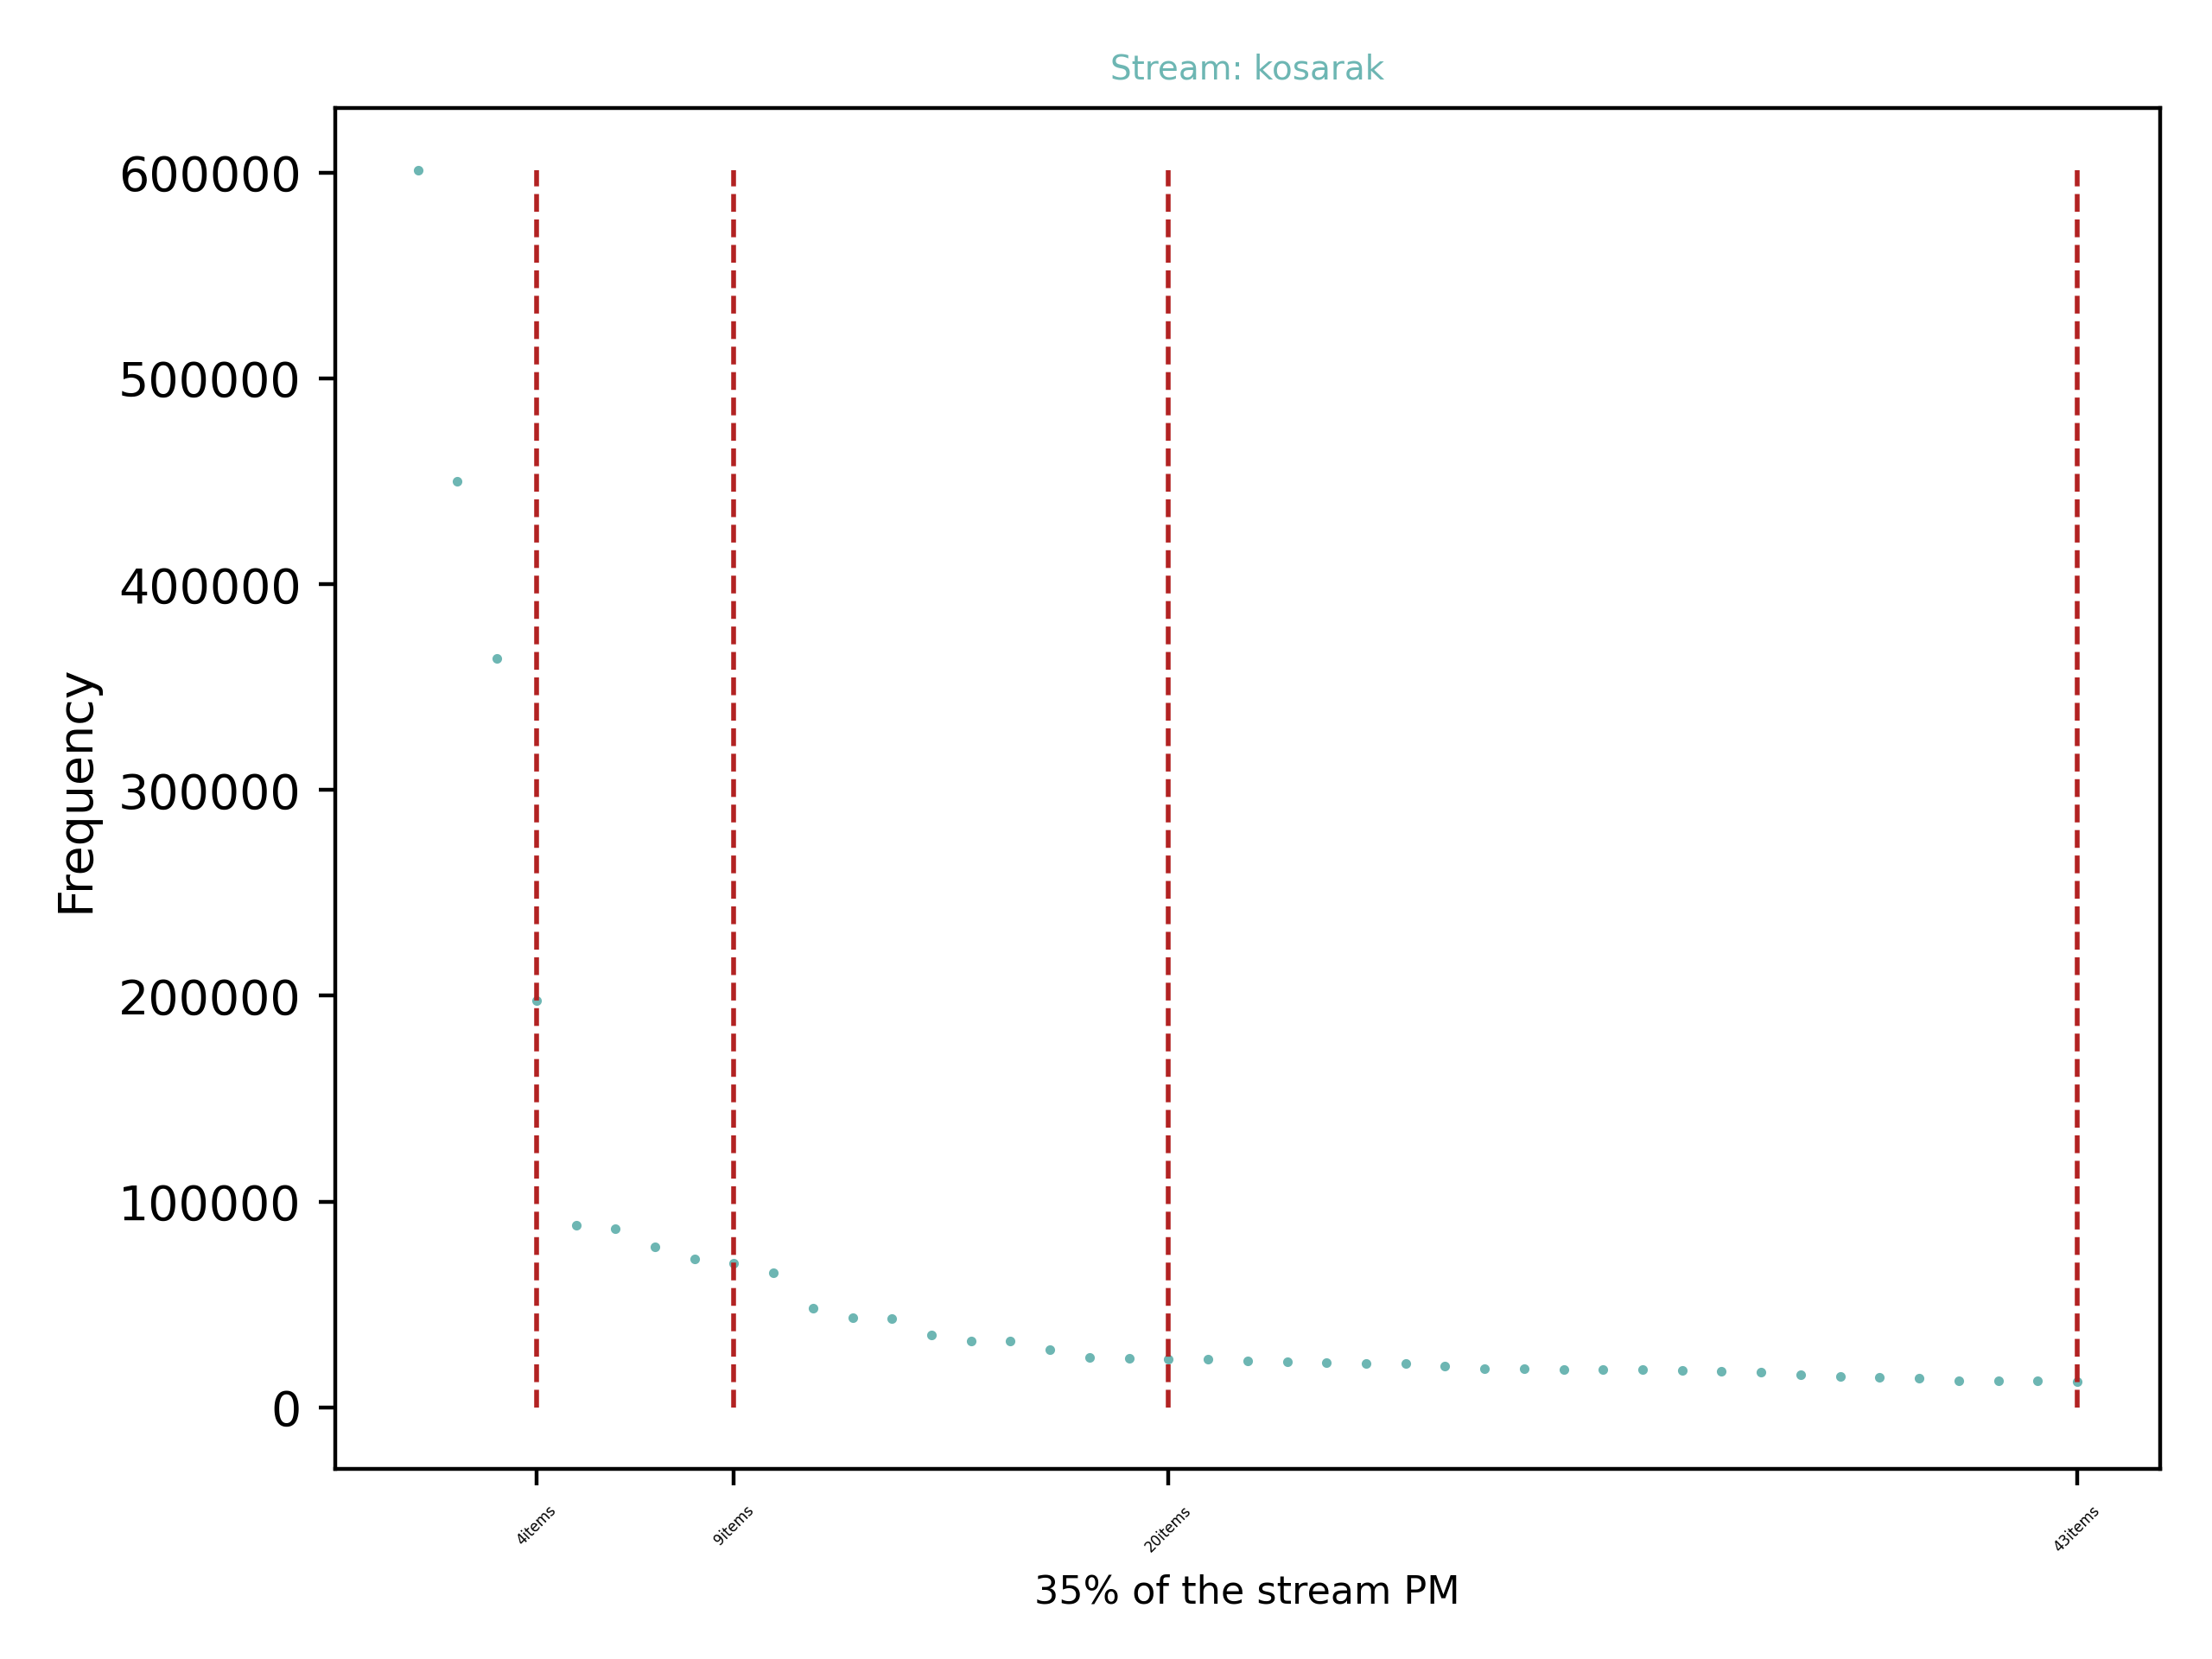
\includegraphics[width=\linewidth]{chapters/ch3_cfe/images/kosarak_pm.png}
    \caption*{Kosarak stream}
  \endminipage\hfill
  \minipage{0.32\textwidth}
    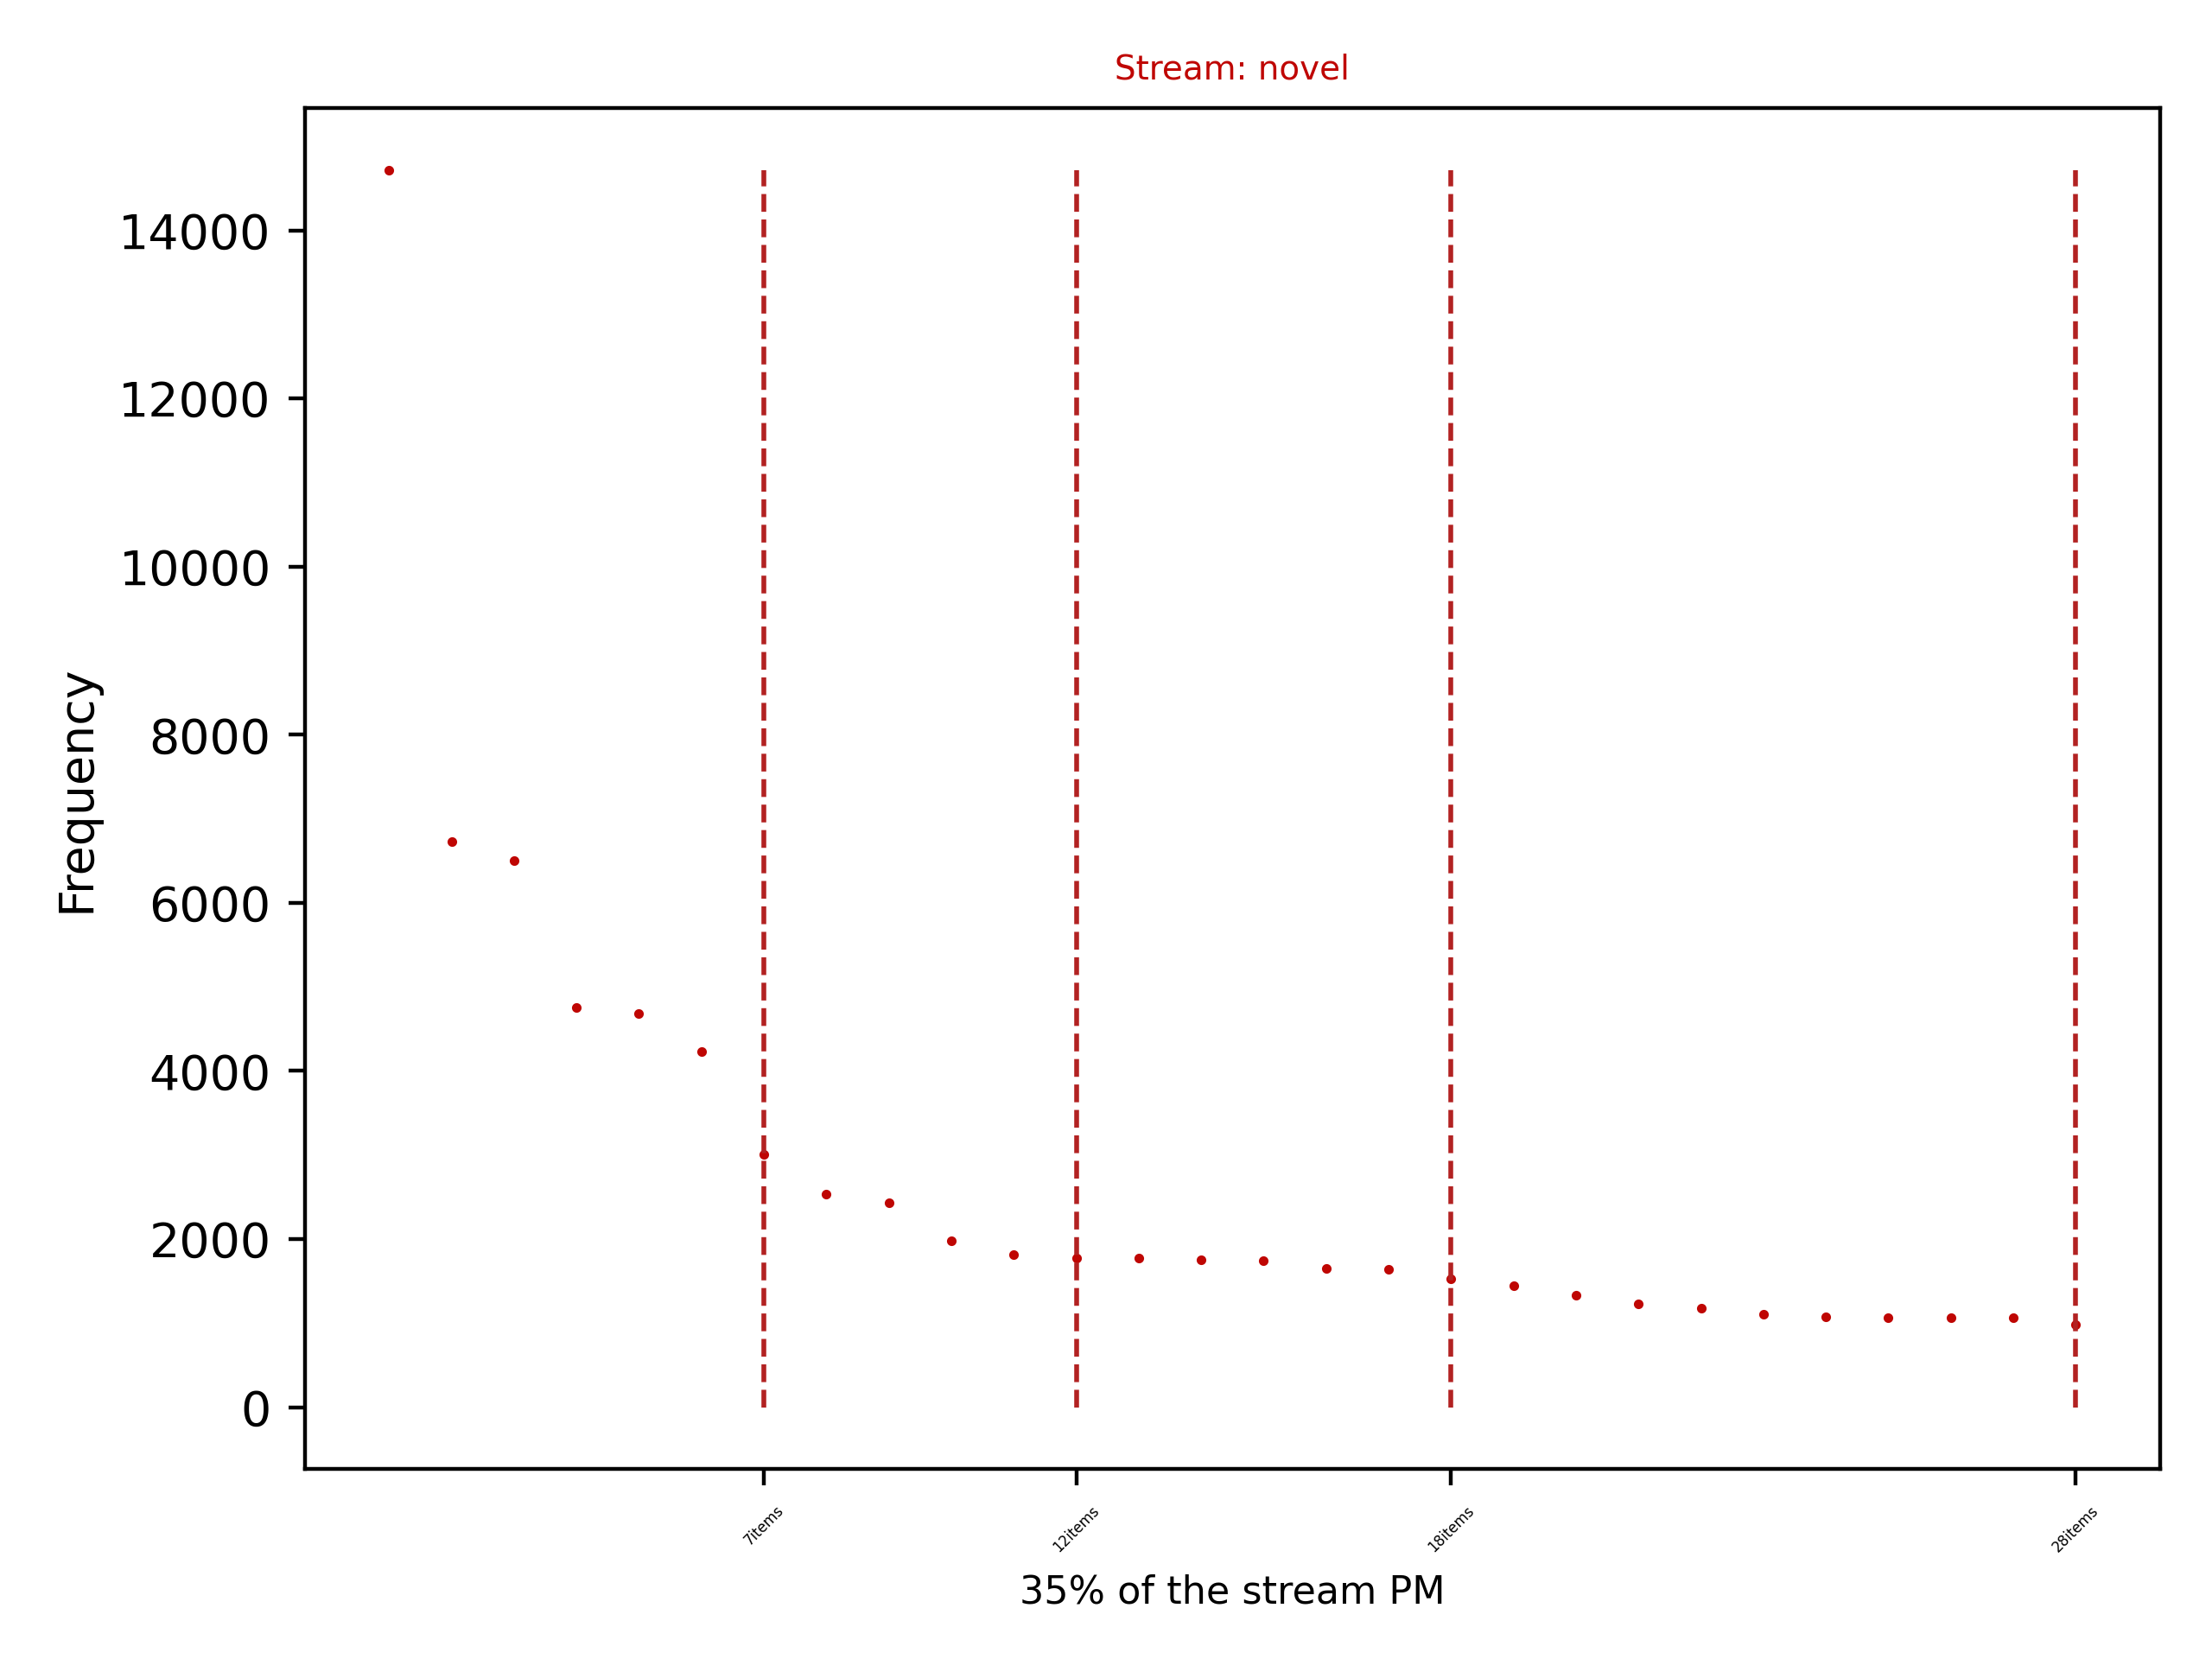
\includegraphics[width=\linewidth]{chapters/ch3_cfe/images/novel_pm.png}
    \caption*{Novel stream}
  \endminipage\hfill
  \minipage{0.32\textwidth}%
    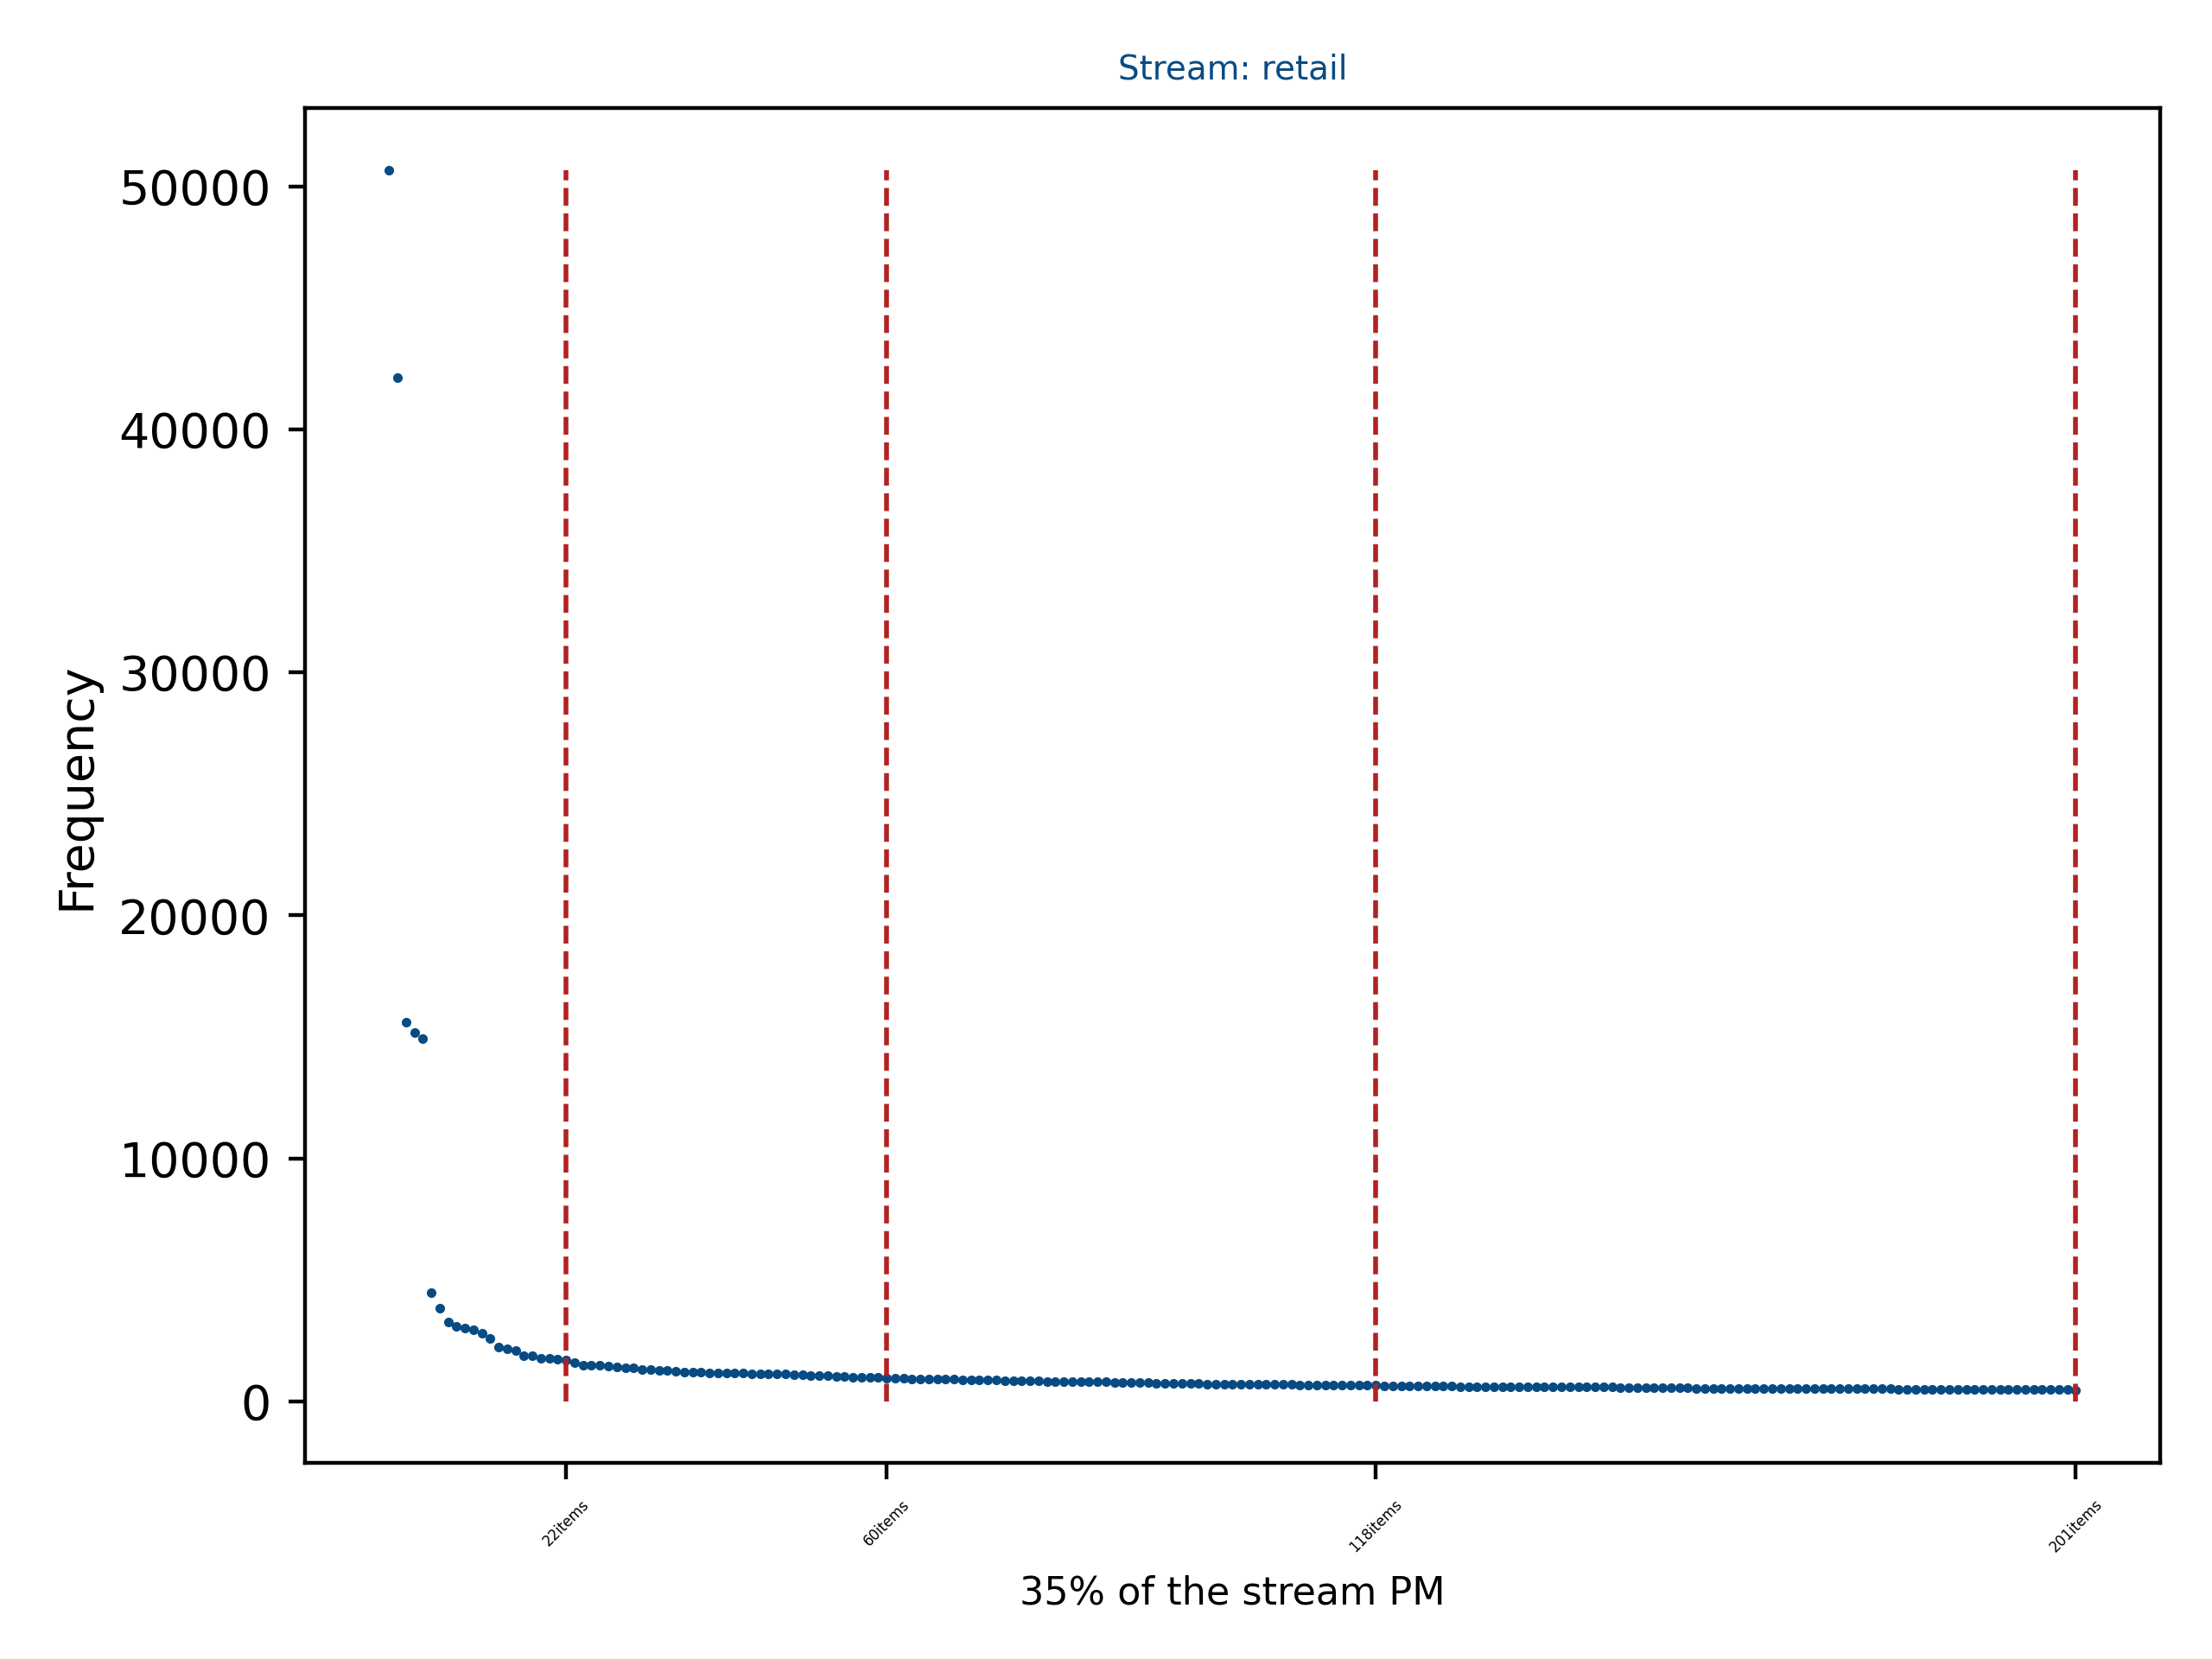
\includegraphics[width=\linewidth]{chapters/ch3_cfe/images/retail_pm.png}
    \caption*{Retail stream}
  \endminipage
  \caption[Stream Frequent Elements.]{We plot the top~$35\%$ probability mass for each stream. That is the most frequent elements that make up~$35\%$ of the total weight of the stream (i.e. the fewest number of elements in each stream whose frequencies sum to such that when divided by the total length of the stream equal~$35\%$). The first vertical red line in each plot is the top~$20\%$ probability mass, the second the top~$25\%$, the third the top~$30\%$, and the last the top~$35\%$. From visual inspection we decided to make the top-$K$ cut-off at, $20$ for Kosarak stream, $22$ for the Novel stream, and~$22$ for the Retail stream.}
  \label{fig:stream_pm} 
\end{figure*}
\paragraph{Measures and Metrics} We want to measure the performance of the CFEs of interest in the non-adversarial setting by determining how well they are able to identify and characterize the heavy elements in the streams above. %\mia{Why is it satisfactory to do it that way - aka test the streams only on limited number of streams? (if not addressed before)}

This problem, with varying but related definitions, is referred to in the literature as the heavy-hitters problem, the hot-items problem, or the top-$K$ problem. 

%\mia{[style] I think the sentence can be written better. 'to apply' - what do we actually mean by that? Can we be more concrete when giving the definition- possibly giving a bit more math-looking one as we have for some other stuff OR reference to a paper with it? }
The simplest of these definitions to apply is that of the top-$K$ problem, which is to simply report the set of elements with the~$K$ highest frequencies (for some~$K$) for a given stream. That is given elements of a stream~$\streamvar{S} \subseteq  \{ e_1,e_2,\ldots,e_M \}$ with associated frequencies~$(n_{e_1},n_{e_2},\ldots,n_{e_M})$ we can order the elements~$\{ e^{*}_{1},e^{*}_{2},\ldots,e^{*}_{M} \}$ such that~$(n^{*}_{e_1} \geq n^{*}_{e_2} \geq \ldots \geq n^{*}_{e_M})$. Then for some~$K \in \mathbb{Z}^{+}$ we output the set of elements~$\{ e^{*}_{1},e^{*}_{2},\ldots,e^{*}_{K} \}$ with the~$K$ highest frequencies~$(n^{*}_{e_1} \geq n^{*}_{e_2} \geq \ldots \geq n^{*}_{e_K})$.

The top-$K$ problem can be solved exactly given space linear to that of the stream by keeping an individual counter for each distinct element in the stream. It is not possible to solve exactly with space less than linear (see~\cite{Roughgarden_Valiant} for a formal impossibility argument), but it is a common technique to place a small data structure such as a min-heap restricted to size~$K$ on top of a CFE and by updating this small structure on each insertion once, one is able to approximate this top-$K$ set~\cite{yang2019heavykeeper,mandal2018topkapi,metwally2006}.

%\mia{How do we know this? Is it a common knowledge for CFE ppl - if so state it as such and give your source for the info.}. 

For our purposes we simply compute the approximate top-$K$ by processing the stream with a compact frequency estimator, querying on every distinct element in the stream, and ordering elements by approximated frequency. Likewise, we compute a true top-$K$ for each stream by processing said stream with a map linear in the size of the stream, computing a frequency for each element, and ordering by true frequency.  We note that we would have achieved identical results by putting a min-heap on top of each structure with fixed sized~$K$, updating as described in~\cite{yang2019heavykeeper} and outputting its contents once the entire stream has been processed. However, for experimental purposes our approach is more extensible than the one that would be used in practice.

%\mia{why don't we also consider the heap - this is possibly tom todo, why the alternative approach, what are its strengths (and weaknesses). How do we justify accepting the weaknesses?}

The number of heavy elements, or perhaps the number of heavy elements one would care about, varies depending on the stream and the application. For instance, it is noted that in a telecommunications scenario when monitoring the top outgoing call destinations of a customer typically a value of~$K$ in the range of~$10-20$ is appropriate~\cite{homen2010}. Moreover, when identifying the most frequent elements of interest of Zipfian distribution it is often of interest to vary~$K$ based on the parameters of the underlying distribution~\cite{charikar2002finding}.

We select~$K$ for each stream by observing the number of clearly identifiable outliers in the underlying stream.  We do this by visually inspecting the selected streams' frequency plots. We set the $x$-axis to enumerate all distinct elements in a stream, ordered from  most to least frequent and the $y$-axis as those distinct elements' corresponding frequencies. We make a cut-off around the point where the frequencies went from very peaked (distinct with prominent frequency jumps from element to element) to flat (many elements with about the same frequency -- the point at which the frequency differences decline less sharply). These frequency plots can be seen in Figure~\ref{fig:stream_pm}. We set~$K=20$ for the Kosarak stream,~$K=22$ for the novel stream, and~$K=22$ for the retail stream. 

We measure the accuracy of the non-adversarial performance according to four different metrics.

\begin{enumerate}[wide, labelwidth=!, labelindent=0pt]
    \item \textbf{Set Intersection Size (SIS):} This measures the size of the set intersection of the true top-$K$ set~$\set{K}$ of the stream and the estimated top-$K$ set~$\tilde{\set{K}}$ as reported by the CFE:~$\text{SIS} = |\set{K} \cap \tilde{\set{K}}|$. This is measure of precision on the estimated top-$K$ set as compared to the true top-$K$ set. A SIS of~$K$ would imply perfect precision. 
    
    \item \textbf{Jaccard Index (JI):} The JI is a statistic that measures the similarity of two sets~\cite{real1996probabilistic}. We use the statistic to determine the similarity of the true top-$K$ set~$\set{K}$ of the stream and the estimated top-$K$ set~$\tilde{\set{K}}$ as reported by the CFE. It is defined as~$\mathrm{JI} = \frac{|\set{K} \cap \tilde{\set{K}}|}{|\set{K} \cup \tilde{\set{K}}|}$. A JI can be in the range~$[0,1]$, with a JI of~$1$ implying a perfect characterization of the true top-$K$ set by the CFE in its top-$K$ estimation. 
    
    \item \textbf{Minimal Top-$\tilde{K}$ to Capture True Top-K (MCT):} 
    This measures determines the minimal size~$L \geq K$ the estimated top-k set~$\tilde{\set{K}}$ would need to be to capture all elements contained in the true top-$K$ set~$\set{K}$. That is if one were to order the frequency estimates of all items made by a particular CFE, we would determine the number of items one would need to examine (starting from the most-frequent going down to the least-frequent) until all the elements from~$\set{K}$ were contained in that ordered set. Thus,~$L-K$ indicates the number of elements that fall out of~$\set{K}$ that are incorrectly being individually estimated to be greater than at least one element that is truly in~$\set{K}$. 
    
    \item \textbf{Average Relative Error on Top-k  elements (ARE)}:
    Average Relative Error is a standard measure to use when comparing CFEs~\cite{yang2019heavykeeper}. It is defined as~$\mathrm{ARE} = \frac{1}{K} \sum_{i=1}^{K} \frac{| \hat{n_{i}} - n_{i}|}{n_{i}}$
    where $i \in [K]$ indexes the true top-$K$ elements for a particular stream.
\end{enumerate}

\paragraph{Results} We crafted reference implementations for all three CFEs of interest: CMS, HK, and CK\footnote{Source code is available at: \url{https://github.com/smarky7CD/cfe-in-adv-envs}}. They are implemented in Python3 and use the BLAKE2b cryptographic hash function %(a 64-bit output hash) 
for independent row hash functions and for a fingerprint hash function in the case of CK and HK. %\mia{How big are fps and cnts? Or is it a parameter that a person running our implementation can vary?} \smnote{Technically, unbounded due to Python, but all remain under 32 bits in size in practice .}

We are interested in comparing performance when the space used by the structures is held constant. Observe that CK is three times as large as  CMS, and HK is twice as large as CMS assuming the same space is used for a counter bucket and a fingerprint bucket (in the CK and HK) across all structures. In practice these buckets could be (say)~$32$-bits. We picked two sets of parameters, a \emph{standard} set and a \emph{constrained} set to test.

The standard set of parameters set~$m=2048,k=4$ for CMS,~$m=1024,k=4$ for HK, and~$m=910,k=3$ for CK. This corresponds to~$32.76$~kB of space when using a 32-bit bucket sizes. We experimentally show that at this size all the structures are able to identify the heavy elements of the streams we test upon with minimal to no error. 

The constrained set of parameters sets~$m=512,k=4$ for CMS,~$m=256,k=4$ for HK, and~$m=341,k=2$ for CK. This corresponds to just~$8.19$~kB of space when using a 32-bit counter and fingerprint bucket sizes. In this space constrained setting the structures are still able to identify the heavy elements of the streams we test upon, but with some degree of moderate error. 

For HK, we set~$d=0.9$ for all experiments, as this is the default chosen by Redis~\cite{redisbloom} and satisfies the desired properties of the exponential decay function stated in~\cite{yang2019heavykeeper}. 

We ran~$1000$ trials for each structure, stream, and parameter triplet using our reference implementations. We randomize each trial on the particular choice of hash functions used for the rows (by selecting a random per-trial seed), as well as the order in which the items in the stream are processed. The latter simulates an item being randomly drawn from the underlying distribution of the stream. We averaged our four metrics for each structure, stream and parameter triplet over the~$1000$ trials. 

\begin{table*}[!ht]
  \centering
  \begin{tabular}{|ccccccc|}
  \hline
  \multicolumn{1}{|c|}{\textbf{Structure}} & \multicolumn{1}{c|}{\textbf{\begin{tabular}[c]{@{}c@{}}Parameters\\ (m,k)\end{tabular}}} & \multicolumn{1}{c|}{\textbf{Stream}}                                                                   & \multicolumn{1}{c|}{\textbf{SIS}}                                                     & \multicolumn{1}{c|}{\textbf{JI}}                                                   & \multicolumn{1}{c|}{\textbf{MCT}}                                                      & \textbf{ARE}                                                  \\ \hline
  \multicolumn{7}{|l|}{\textit{Standard}}                                                                                                                                                                                                                                                                                                                                                                                                                                                                                                                                               \\ \hline
  \multicolumn{1}{|c|}{CK}                 & \multicolumn{1}{c|}{(910,3)}                                                             & \multicolumn{1}{c|}{\multirow{3}{*}{\begin{tabular}[c]{@{}c@{}}Kosarak~($K=20$)\\ Novel~($K=22$)\\ Retail~($K=22$)\end{tabular}}} & \multicolumn{1}{c|}{\begin{tabular}[c]{@{}c@{}}20\\ 22\\ 22\end{tabular}}             & \multicolumn{1}{c|}{\begin{tabular}[c]{@{}c@{}}1\\ 1\\ 1\end{tabular}}             & \multicolumn{1}{r|}{\begin{tabular}[c]{@{}r@{}}20\\ 22\\ 22\end{tabular}}              & \begin{tabular}[c]{@{}c@{}}$\approx 0$\\ $\approx 0$\\ $\approx 0$\end{tabular}             \\ \cline{1-2} \cline{4-7} 
  \multicolumn{1}{|c|}{CMS}                & \multicolumn{1}{c|}{(2048,4)}                                                            & \multicolumn{1}{c|}{}                                                                                  & \multicolumn{1}{c|}{\begin{tabular}[c]{@{}c@{}}19.303\\ 22.999\\ 21.643\end{tabular}} & \multicolumn{1}{c|}{\begin{tabular}[c]{@{}c@{}}0.934\\ 0.999\\ 0.997\end{tabular}} & \multicolumn{1}{r|}{\begin{tabular}[c]{@{}r@{}}20.901\\ 22.001\\ 22.405\end{tabular}}  & \begin{tabular}[c]{@{}c@{}}0.017\\ 0.009\\ 0.040\end{tabular} \\ \cline{1-2} \cline{4-7} 
  \multicolumn{1}{|c|}{HK}                 & \multicolumn{1}{c|}{(1024,4)}                                                            & \multicolumn{1}{c|}{}                                                                                  & \multicolumn{1}{c|}{\begin{tabular}[c]{@{}c@{}}20\\ 22\\ 22\end{tabular}}             & \multicolumn{1}{c|}{\begin{tabular}[c]{@{}c@{}}1\\ 1\\ 1\end{tabular}}             & \multicolumn{1}{r|}{\begin{tabular}[c]{@{}r@{}}20\\ 22\\ 22\end{tabular}}              & \begin{tabular}[c]{@{}c@{}}$\approx 0$\\ $\approx 0$\\ $\approx 0$\end{tabular}             \\ \hline
  \multicolumn{7}{|l|}{\textit{Constrained}}                                                                                                                                                                                                                                                                                                                                                                                                                                                                                                                                               \\ \hline
  \multicolumn{1}{|c|}{CK}                 & \multicolumn{1}{c|}{(341,2)}                                                             & \multicolumn{1}{c|}{\multirow{3}{*}{\begin{tabular}[c]{@{}c@{}}Kosarak~($K=20$)\\ Novel~($K=22$)\\ Retail~($K=22$)\end{tabular}}} & \multicolumn{1}{c|}{\begin{tabular}[c]{@{}c@{}}17.189\\ 21.617\\ 13.442\end{tabular}} & \multicolumn{1}{c|}{\begin{tabular}[c]{@{}c@{}}0.757\\ 0.967\\ 0.441\end{tabular}} & \multicolumn{1}{c|}{\begin{tabular}[c]{@{}c@{}}28.695\\ 22.451\\ 209.439\end{tabular}} & \begin{tabular}[c]{@{}c@{}}$\approx 0$\\ $\approx 0$\\ 0.021\end{tabular}         \\ \cline{1-2} \cline{4-7} 
  \multicolumn{1}{|c|}{CMS}                & \multicolumn{1}{c|}{(512,4)}                                                             & \multicolumn{1}{c|}{}                                                                                  & \multicolumn{1}{c|}{\begin{tabular}[c]{@{}c@{}}18.241\\ 21.638\\ 18.745\end{tabular}} & \multicolumn{1}{c|}{\begin{tabular}[c]{@{}c@{}}0.841\\ 0.969\\ 0.745\end{tabular}} & \multicolumn{1}{c|}{\begin{tabular}[c]{@{}c@{}}24.567\\ 22.473\\ 41.609\end{tabular}}  & \begin{tabular}[c]{@{}c@{}}0.125\\ 0.062\\ 0.296\end{tabular} \\ \cline{1-2} \cline{4-7} 
  \multicolumn{1}{|c|}{HK}                 & \multicolumn{1}{c|}{(256,4)}                                                             & \multicolumn{1}{c|}{}                                                                                  & \multicolumn{1}{c|}{\begin{tabular}[c]{@{}c@{}}20\\ 22\\ 21.976\end{tabular}}         & \multicolumn{1}{c|}{\begin{tabular}[c]{@{}c@{}}1\\ 1\\ 0.998\end{tabular}}         & \multicolumn{1}{c|}{\begin{tabular}[c]{@{}c@{}}20\\ 22\\ 55.008\end{tabular}}          & \begin{tabular}[c]{@{}c@{}} $\approx 0$\\ 0.001\\ 0.005\end{tabular}     \\ \hline
  \end{tabular}
  \caption[Non-adversarial CFE Results.]{A summary of non-adversarial setting results between the CK, CMS, and HK compact frequency estimators.}
  \label{tab:hon-exp-res}
  \end{table*}


We present a summary of the results in Table~\ref{tab:hon-exp-res}. For the \emph{standard} parameter set we see that CK and HK perform best, being able to perfectly capture the true top-$K$ set for each stream with their outputted estimated top-$K$ set in \emph{every} trial. This is indicated by the SIS and MCT being equal to~$K$ and the JI being equal to~$1$ for each stream. Moreover, the estimates on these top-$K$ elements for both of these structures were very tight. The ARE over all trials and streams was~$0$ (ignoring a small rounding error). This indicates that CK and HK nearly perfectly individually estimated every single element in the true top-$K$ across all trials. 
  
CMS with the standard parameter sizing performs almost as well. Only failing to capture the true top-$K$ set with its estimated set a few number of times over the~$1000$ trials. This is indicated by the SIS and MCT being very close to~$K$ and the JI being very close to~$1$ for each stream. However, CMS, as it is prone to overestimation on every element, has slightly higher ARE than the other structures. 

The \emph{constrained} set of parameters presents a challenge for all the CFEs in computing individual frequency estimations on elements in the streams, and as a result computing an accurate estimated top-$K$. This setting only allocates CK a measly~$642$ individual counters to compactly represent streams that all have over~$19,000$ distinct elements. Under these conditions, HK performs best according to our metrics. It perfectly captures the true top-$K$ in both the Kosarak and Novel stream, while only failing to do so in a handful of trials with the Retail stream. Moreover, the ARE is small across all streams -- comparatively less than CMS with the standard parameters. HK by design prioritizes providing accurate estimates on the most frequent elements, by way of its probabilistic decay mechanism. So while it performs well on this task, it severely underestimates middling and low frequency elements at this sizing, reporting an individual frequency estimate very near~$0$ for any element that is not heavy. %This behavior is what we exploit in our attacks to create error in the structure, effectively masking true heavy elements. 

 CMS and CK perform less well in this small space allocation setting. While CMS performs slightly better in capturing the true top-$K$ set within its estimated top-$K$ set, CK continues to give better accuracy on individual point estimations of the true top-$K$ elements across streams due to its internal sub-estimators that provide tighter estimations than CMS.

We observe in this constrained space setting across the structures measured performance is the worst on the Retail stream. This is because the Retail stream has a flatter distribution as compared to the other streams. That is to say, it has very few clearly identifiable heavy elements before containing a large collection of elements of about the same frequency. This can be seen in the frequency plot in Figure~\ref{fig:stream_pm}. The Retail element with frequency rank~$22$ has a true frequency of~$1715$ while the Retail element of frequency rank~$56$ has a true frequency of~$1005$. Comparing this to $n_{22} = 22631, n_{56} = 9559$ and~$n_{22} = 1176, n_{56} = 474$, respectively for the Kosarak and Novel stream, one can see that the relative fall off in true frequency is far less pronounced within this region of the Retail stream. This in turn leads to small errors in the individual frequency estimations of elements near (but outside) the true top-$K$ of the Retail stream propagating to the top-$K$ estimation -- by making it challenging for the CFEs to draw a clear distinction between the truly heavy elements and the nearly heavy elements. The upshot being, one needs larger structures to accurately estimate these flatter streams.

In sum, CK performs comparatively well to both CMS and HK in this particular task. In fact, CK performed better than CMS when not burdened with \emph{very} tiny space constraints. It is able to perfectly estimate the true top-$K$ for all streams over all trials with only $2730$ individual counters in the standard parameter setting, while also being adversarial robust where the others structures are not. 



\subsection{Attacks Against the CK}\label{sub-sec:ck-attacks}
Our attacks against CK are almost one-to-one with those we present against the CMS with one major difference. Recall from Corollary~\ref{cor:fx:MA:Theta13:nx} that if at least one counter in some row~$i$ of the element~$x$ we are querying on maps to has~$|V^i_x| \leq 1$ then CK returns estimate~$\hat{n}_x$ such that~$\hat{n}_x = n_x$, i.e. $\CK(x)$ is a perfect estimate of~$x$. This implies that for an error to exist in a frequency estimation of~$x$ it must be that~$\forall i \in [k]$ it is necessary that~$|V^i_x| \geq 2$. In the attack setting this means we need to find a $2$-cover (specifically a~$(\set{FP}_{x},x,2)$-cover) on~$x$ to create error.

A 2-cover~$\set{C}$ for~$x$ contains elements~$\{y_1,y_2,\ldots,y_t\}$ such that for every counter $x$ maps to in positions~$(p_1,p_2,\ldots,p_k) \gets R(K,x)$ it is such that at least two distinct elements in~$\set{C}$ cover each counter. In our attack model we assume an initially empty representation and we never insert~$x$ in any of our attacks (except for once to discover its counter positions in the public representation, private hash setting). 

We attack CK in a two-step process, as with CMS and HK. We first find a 2-cover for our target element~$x$ and then repeatedly insert the 2-cover to create error. Under the assumption that~$x$ does not own any of its counters in the~$A$ substructure of the CK (which is guaranteed in our attack model\footnote{Save for the trivial case in the public representation, private hash setting when no cover is able to be found.}), then the~$\Theta_1$ sub-estimator will be used to make the final error evaluation~$\QRYO$ query on~$x$. Say that after some process of finding a 2-cover for~$x$ (which will be of size~$\leq 2k$ -- for this discussion we will assume the size of the 2-cover is exactly~$2k$) we have~$\omega$ insertions to repeatedly insert the elements in the cover. Repeated and equal insertions of each of the elements in the 2-cover for~$x$ will cause the values in all of $x$'s counters in the~$M$ substructure of the CK to be of value~$\frac{\omega}{k}$. In the~$A$ substructure the value in the counters that~$x$ maps to will have value~$1$ and be owned by some element in the 2-cover. This is because (under the no-fingerprint collision assumption) in the initially empty structure, ownership of said counters will flip-flop on each iteration of the insertions of the 2-cover between the two distinct elements that map to these counters in accordance with the~$\Up$ algorithm of the HK with~$d=1$. 

Then applying the estimation from~$\Theta_1$ we see that we will generate error on~$x$ equal to~$\frac{\omega}{2k}$. If we hold~$k$ constant and assume that we are attacking a CMS under the same conditions (we have found a 1-cover for a target~$x$ through some process and have~$\omega$ insertions to accrue error) we will have an error of~$\frac{\omega}{k}$, which is twice that of the CK under the same conditions. Under the same assumptions for HK, in addition to the assumption that we have already locked-down the counters of the target with initial insertions of the cover in the structure, we will achieve an error on the target of~$\omega$ -- which is~$\omega - \frac{\omega}{2k}$ greater than that of the CK. We will see this pattern holds when giving concrete experimental attack error results at the conclusion of this section.

\paragraph{Public hash and representation setting}
\begin{figure*}[ht!]
	\Wider[2em]{
		\centering
		\begin{pchstack}[boxed,center,space=0.4em]
			\procedure[linenumbering, headlinecmd={\vspace{.1em}\hrule\vspace{.2em}}]{$\text{CoverAttack}^{\HASHO,\UPO,\QRYO}(x, K, {\repr})$}{%
				\textrm{cover} \, {\gets} \textrm{FindCover}^{\HASHO}(2,x,K)\\
				\pcuntil q_U \ \UPO \text{-queries made:}\\
				\t \pcfor e \in \textrm{cover}{:} \ \UPO(e)\\
				\pcreturn \textrm{done}
			}
			\procedure[linenumbering, headlinecmd={\vspace{.1em}\hrule\vspace{.2em}}]{$\text{FindCover}^{\HASHO}(r, x, K)$}{%
				\textrm{cover} \gets \emptyset; \,
				\textrm{found} \gets \mathsf{False}\\
				\set{I} \gets \emptyset; \,\textrm{tracker} \gets \zeros(k)\\
				\hspace{-.5em}
				\pcgraycomment{$R(K,x)[i]=\HASHO(\encode{i,K,x})$}\\
				(p_1,p_2,\ldots,p_k) \gets R(K,x)\\
				\pcwhile \textrm{not found}\\
				\t \pcif q_H \ \HASHO\text{-queries made}\\
				\t \t \pcreturn \emptyset\\
				\t y \getsr \set{U}\setminus (\set{I} \cup \{x\})\\
				\t \set{I} \gets \set{I} \cup \{y\}\\
				\t (q_1,q_2,\ldots,q_k) \gets R(K,y)\\
				\t \pcfor i \in [k]\\
				\t \t \pcif p_i = q_i~\textbf{and}~\textrm{tracker}[i] < r\\
				\t \t \t \textrm{cover} \gets \textrm{cover} \cup \{y\}\\
				\t \t \t \textrm{tracker}[i]~+= 1\\
				\t \pcif \mathsf{sum}(\textrm{tracker}) = rk\\
				\t \t \textrm{found} \gets \mathsf{True}\\
				\pcreturn \textrm{cover}
			}
		\end{pchstack}
	}
	\caption{Cover Set Attack for the CK in public
		hash function setting. 
%		We use $R(K,x)$ to mean $(\HASHO(\encode{1,K,x}),\HASHO(\encode{2,K,x},\ldots,\HASHO(\encode{k,K,x})))$.
		The attack is parametrized with  the update and $\HASHO$ query budget $q_U$ and $q_H$.
	}
%\mia{The attck is 1-1 with CMS attack (Figure \ref{fig:attack-cms-hfcs}) with $\textrm{FindCover}^{\HASHO}(1,x,K)$ changing to $\textrm{FindCover}^{\HASHO}(2,x,K)$ (first line of the code)! So, I think that we do NOT need this code in the paper.}
	\label{fig:attack-ck-hf2cs}
\end{figure*}
As our other attacks (for CMS and HK) in this setting, the CK attack (Figure~\ref{fig:attack-ck-hf2cs}) can be viewed as a two-step process.  In this setting, we find a 2-cover for target~$x$ using the $\HASHO$ oracle only, and then accumulate error for the target by repeatedly inserting the 2-cover. Each insertion of the 2-cover increases the error by one. The two cover can be inserted at least $\frac{q_U}{2k}$ as the size of the cover is~$\leq 2k$.
We apply the same analysis used for the CMS attack, but replace $k(1 + L^1)$ with $k(1 + L^2)$ as the number of $\HASHO$-queries to complete the cover-finding step, as again, we now find a 2-cover. Assuming $q_U > 2k$ (so that any found $\set{C}$ can be inserted at least once)
we arrive at
%\begin{align}\label{eqn:pub-pub-pr-cover-qH-CK}
$\mathbb{E}[\rverr] \geq \left\lfloor\frac{q_U}{2k}\right\rfloor \Pr\left[L^2 \leq \frac{q_H-k}{k}\right]$
%\end{align}
Using results from Section \ref{sec:cov-set} we can further obtain a concrete expression for $\Pr\left[L^2 \leq \frac{q_H-k}{k}\right]$. 

\paragraph{Private hash and representation setting}
\begin{figure*}[ht!]
	%\Wider[2em]{
		\centering
		\begin{pchstack}[boxed,center,space=0.5em]
		\begin{pcvstack}[space = 0.45em]
	\procedure[linenumbering, headlinecmd={\vspace{.1em}\hrule\vspace{.2em}}]{$\text{CoverAttack}^{\UPO,\QRYO}(x, \bot, \bot)$}{%
		\textrm{cover} \gets \textrm{FindCover}^{\UPO,\QRYO}( x)\\
		\pcuntil q_U \ \UPO \text{-queries made:}\\
		\t \pcfor e \in \textrm{cover}{:} \ \UPO(e)\\
		\pcreturn \textrm{done}
	}
	\procedure[linenumbering, headlinecmd={\vspace{.1em}\hrule\vspace{.2em}}]{$\text{MinUncover}^{\UPO,\QRYO}(x, a', \text{cover})$}{%
		b' \gets a' - 1\\
		\pcwhile a' \not= b'\\
		\t \pcif (q_U-|\textrm{cover}| + 1)\UPO\text{-} \\
		\t \t \text{ or } q_Q \ \QRYO\text{-queries made:}\\
		\t \t \t \pcreturn \textrm{cover}\\
		\t b' \gets a'\\
		\t \pcfor y \in \text{cover}: \UPO(y)\\
		\t a' \gets \QRYO(x)\\
		\pcreturn a'
	}
\end{pcvstack}
\procedure[linenumbering, headlinecmd={\vspace{.1em}\hrule\vspace{.2em}}]{$\text{FindCover}^{\UPO,\QRYO}(x)$}{%
	\pcgraycomment{find $2$- cover for x}\\
	\textrm{cover} \gets \emptyset\\
	\textrm{found} \gets \mathsf{False}\\
	%			; \textrm{lessened} \gets \mathsf{False}\\
	\set{I} \gets \emptyset; a \gets \QRYO(x) \\
	\hspace{-.5em}
	\pcwhile \textrm{not found} \\
	\t \pcif q_U \ \UPO \text{- or } q_Q \ \QRYO\text{-queries made}\\
	\t \t \pcreturn \textrm{cover}\\
	\t y \getsr \univ \setminus (\set{I} \cup \{x\})\\
	\t \set{I} \gets \set{I} \cup \{y\}\\
	\t \UPO(y); \ a' \gets \QRYO(x)\\
	\t \pcif a' \not= a: \\
	\t \t \textrm{cover} \gets \{y\}\\
	\t \t \textrm{found} \gets \mathsf{True}\\
	\pcfor i \in [2, 3, \dots, 2 \cdot k]\\
	\t a \gets \text{MinUncover}^{\UPO,\QRYO}(x, a', \text{cover}) \\
	\t \pcif a = \textrm{cover}: \pcreturn \textrm{cover}\\
	\t \pcfor y \in \set{I} \ \pcgraycomment{in order of insertion to $\set{I}$}\\
	\t \t \pcif q_U \ \UPO \text{- or } q_Q \ \QRYO\text{-queries made}\\
	\t \t \t \pcreturn \textrm{cover}\\
	\t \t \UPO(y); a' \gets \QRYO(x) \\
	\t \t \pcif a' \not= a: \\
	\t \t \t \textrm{cover} \gets \textrm{cover} \cup \{y\}\\
	%			This is just here so the algorithm is exactly the same for the CK!
	\t \t \t \set{I} \gets \set{I} \setminus \{y\}\\
	\t \t \t \textbf{break}\\
	\pcreturn \textrm{cover} \ \pcgraycomment{cover is inserted at least once}
}
\end{pchstack}
		%}
	\caption{Cover Set Attack for the CK in private
		hash function and representation setting. 
		The attack is parametrized with the update query and query query budget -- $q_U$ and $q_Q$.}
%\mia{The attck is 1-1 with CMS attack (Figure \ref{fig:attack-cms-iqcsa}) with $\textrm{FindCover}^{\UPO,\QRYO}(x)$, line \ref{alg:CMS:CK:change} changing to go up to $2k$! This is because we are now finding a two cover! Overall, I think that we do NOT need this code in the paper.}
%\mia{@Sam I am hesitant to define $\textrm{FindCover}^{\UPO,\QRYO}(x)$ with argument $r$. I do not see if taking the algorithm with $r!=2$ would make any sense for CK (would find $r$ cover, even for $r=4$), or that the algorithm with $r!=1$ actually finds an $r$-cover for CMS.}
%\mia{Is \textrm{FindCover} alg. name collision between the CMS and CK attack too confusing? (irrelevant if we do not have the code in the paper.)}
	\label{fig:attack-ck-iq2csa}
\end{figure*}

Our CK attack for the setting (Figure~\ref{fig:attack-ck-iq2csa}) is essentially the same as the CMS attack, except a 2-cover (as opposed to a 1-cover) is detected and repeatedly inserted to build up the error. Using analysis similar to the CMS case and assuming~$q_Q$ is not the limiting factor,

$$\rverr \geq 
	\left \lfloor \left( \frac{\ell+1}{2} + \frac{1}{\ell}\left(q_U + \sum_{i=1}^{\ell-1}(\ell-i)\delta_i \right) - L^2 \right) \right\rfloor$$

with~$\ell \leq 2k$ rounds to find a 2-cover. The error bound is similar to the one for the CMS attack, but with $L^1$ replaced with $L^2$ as now $|\streamvar{I}|$ is precisely~$L^2$.  

For reasonable sizes of the CK we mainly expect $\ell = 2k$ (for the CMS case we expected $\ell{=}k$) and that $\mathbb{E}\left[\delta_1\right]$ are bounded by a constant that is small relative to $m, q_U/k$. Given that $k \ll m$, we expect the following to approximate $\mathbb{E}[\rverr]$:
\begin{align*}
	&\mathbb{E}\left[\left\lfloor \left( \frac{2k+1}{2} + \frac{1}{2k}\left(q_U + \sum_{i=1}^{2k-1}(2k-i)\delta_i \right) - L^2 \right) \right\rfloor\right]\approx \frac{q_u}{2k} -  \mathbb{E}[L^2].
\end{align*}

\paragraph{Public hash and private representation setting}
As with the CMS, the attack and analysis from the public hash and representation setting applies.

\paragraph{Private hash and public representation setting}
This attack (Figure~\ref{fig:attack-ck-io2csa}) is one-to-one with the CMS attack in the same setting, but again we find 2-cover as opposed to a 1-cover. Hence,
$\mathbb{E}[\rverr] \geq \frac{q_U-1-\mathbb{E}\left[L^2\right]}{2k} \gtrapprox \frac{q_U-1-2mH_k}{2k}.
$
%$
%\mathbb{E}[\rverr] \geq \Pr[L^2 \leq \ell_U - 1] \left(\floor(\frac{q_U-\ell_U}{2k}) + 1\right)
%$
\begin{figure*}[ht!]
	\centering
	\begin{pchstack}[boxed,center, space=0.5em]
		\procedure[linenumbering, headlinecmd={\vspace{.1em}\hrule\vspace{.2em}}]{$\text{CoverAttack}^{\UPO,\QRYO}(x, \bot, \repr)$}{%
			\textrm{cover} \gets \textrm{FindCover}^{\UPO}(2,x, \repr)\\
			\pcuntil q_U \ \UPO \text{-queries made:}\\
			\t \pcfor e \in \textrm{cover}{:} \ \UPO(e)\\
			\pcreturn \textrm{done}
		}
		\procedure[linenumbering, headlinecmd={\vspace{.1em}\hrule\vspace{.2em}}]{$\text{FindCover}^{\UPO}(r, x, \repr)$}{%
			\left<M, A\right> \gets \repr\\
			\textrm{cover} \gets \emptyset; \,
			\textrm{found} \gets \mathsf{False}\\
			\set{I} \gets \emptyset; \,\textrm{tracker} \gets \zeros(k)\\
			\left<M', A'\right> \gets \UPO(x)\\
			\pcgraycomment{compute $x$'s indices}\\
			\pcfor i \in [k] \\
			\t \pcfor  j \in [m]\\
			\t \t \pcif M'[i][j] \not= M[i][j]\\
			\t \t \t  p_i \gets j; \textbf{break};\\
			\hspace{-.5em}
			\pcwhile \textrm{not found}\\
			\t \pcif q_U \ \UPO\text{-queries made}:\pcreturn \emptyset\\
			\t y \getsr \set{U}\setminus (\set{I} \cup \{x\})\\
			\t \set{I} \gets \set{I} \cup \{y\}\\
			\t  \left<M, A\right> \gets \left<M', A'\right> \\
			\t \left<M', A'\right>  \gets \UPO(y) \\
			\t \pcgraycomment{compute $y$'s indices}\\
			\t \pcfor i \in [k] \\
			\t \t \pcfor  j \in [m]\\
			\t \t \t \pcif M'[i][j] \not= M[i][j]\\
			\t \t \t  \t q_i \gets j; \textbf{break};\\
			\t \pcfor i \in [k]\\
			\t \t \pcgraycomment{compare $x$'s and $y$'s indices row by row}\\
			\t \t \pcif p_i = q_i~\textbf{and}~\textrm{tracker}[i] < r\\
			\t \t \t \textrm{cover} \gets \textrm{cover} \cup \{y\}\\
			\t \t \t \textrm{tracker}[i]~+= 1\\
			\t \pcif \mathsf{sum}(\textrm{tracker}) = rk\\
			\t \t \textrm{found} \gets \mathsf{True}\\
			\pcreturn \textrm{cover}
		}
	\end{pchstack}
	\caption{Cover Set Attack for the CK in private
		hash function and public representation setting. 
		The attack is parametrized with  the update query budget $q_U$.
	}
	%\mia{The attck is 1-1 with CMS attack (Figure \ref{fig:attack-cms-iocsa}) with $\textrm{FindCover}^{\UPO,\QRYO}(1,x,\repr=M)$ changing to $\textrm{FindCover}^{\UPO,\QRYO}(2,x,\repr=\left<M,A\right>)$ (first line of the code), and algorithm FindCover only using CMS's part ('half') of the representation to find element's indices (or similarly HK's part of the representation - it is equivalent). So,do we need this code in the paper?}
	\label{fig:attack-ck-io2csa}
\end{figure*}

\paragraph{Attack Comparisons}
\begin{table*}[htb!]
	\centering
	\begin{tabular}{|c|ccc|ccc|}
	\hline
						 & \multicolumn{3}{c|}{\textbf{Public Hash Setting}}                                                                & \multicolumn{3}{c|}{\textbf{\begin{tabular}[c]{@{}c@{}}Private Hash,\\ Private Rep Setting\end{tabular}}}       \\ \hline
	\textbf{Structure}   & \multicolumn{1}{c|}{$|\mathrm{cover}|$} & \multicolumn{1}{c|}{Experimental~$\rverr$} & $\mathbb{E}[\rverr]$ & \multicolumn{1}{c|}{$|\mathrm{cover}|$} & \multicolumn{1}{c|}{Experimental~$\rverr$} & $\mathbb{E}[\rverr]$ \\ \hline
	$\CK,(m=682,k=4)$    & \multicolumn{1}{c|}{$7.96$}             & \multicolumn{1}{c|}{$131821.00$}                & $131072.00$          & \multicolumn{1}{c|}{$7.96$}             & \multicolumn{1}{c|}{$130796.69$}                & $127432.90$          \\ \hline
	$\CMS, (m=2048,k=4)$ & \multicolumn{1}{c|}{$3.99$}             & \multicolumn{1}{c|}{$263017.82$}                & $262144.00$          & \multicolumn{1}{c|}{$3.99$}             & \multicolumn{1}{c|}{$261116.16$}                & $257877.34$         \\ \hline
	$\HK, (m=1024,k=4)$  & \multicolumn{1}{c|}{$3.99$}             & \multicolumn{1}{c|}{$1047502.69$}               & $1047500.00$         & \multicolumn{1}{c|}{$4.0$}              & \multicolumn{1}{c|}{$1038804.55$}               & $1038018.54$        \\ \hline
	$\CK,(m=1365,k=8)$   & \multicolumn{1}{c|}{$15.97$}            & \multicolumn{1}{c|}{$65667.10$}                 & $65536.00$           & \multicolumn{1}{c|}{$15.93$}            & \multicolumn{1}{c|}{$63776.52$}                 & $56618.28$          \\ \hline
	$\CMS, (m=4096,k=8)$ & \multicolumn{1}{c|}{$8.00$}             & \multicolumn{1}{c|}{$131072.00$}                & $131072.00$          & \multicolumn{1}{c|}{$7.99$}             & \multicolumn{1}{c|}{$127029.66$}                & $119939.65$         \\ \hline
	$\HK, (m=2048,k=8)$  & \multicolumn{1}{c|}{$7.96$}             & \multicolumn{1}{c|}{$1046434.76$}               & $1046424.00$         & \multicolumn{1}{c|}{$7.98$}             & \multicolumn{1}{c|}{$1007439.04$}               & $996946.87$         \\ \hline
	\end{tabular}
	\caption{A comparison of~$\rverr$ accumulated by the different structures during attacks in the public hash setting and the private hash, private representation setting. We give the average size of the cover set and average error accumulated in each structure, setting pair over the~$100$ experiment trials. We also give the~$\mathbb{E}[\rverr]$ according to our analysis. }
	\label{tab:attack-comp}
\end{table*}
We implemented our attacks against all structures in all settings to experimentally verify their correctness and our analysis. In Table~\ref{tab:attack-comp} we present a summary of results for the public hash setting (our least restrictive setting) and the private hash, private representation setting (our most restrictive setting.). We experiment on two sets of parameters, one fixing~$k=4$ and the other~$k=8$. We then select a reasonable value of~$m$ for CMS and then half it for HK and third it for CK so that the same space is used in each structure. We fix adversarial resources such that~$q_H,q_U,q_Q = 2^{20}$. In practice this ensures that the number of~$\HASHO$ queries or~$\QRYO$ queries will not be the bottleneck in our attacks and that we are able to generate sufficient error in each attack to showcase overall trends. We run each attack setting and structure pairing over~$100$ trials, selecting a random target in each trial, and average the results. 

Observe the pattern that when holding~$k$ constant and setting reasonable~$m$ values, adjusting such that CMS, CK, and HK use the same space, attacks against CK generate the least amount of error. The attacks against CK produce about half of the amount of error as opposed to the CMS attacks, and about~$q_U - \frac{q_U}{2k}$ less the amount of error as opposed to the HK attacks. Moreover, observe that our analytical results closely match those of our experimental results. 

\subsection{Adversarial Robustness}\label{sub-sec:ck-flags}
%
\begin{figure*}[h]
	\Wider[3em]{
		\centering
		\begin{pcvstack}[boxed,center,space=0.5em]
			\begin{pchstack}
				\begin{pcvstack}[space=0.45em]
					\procedure[linenumbering, headlinecmd={\vspace{.1em}\hrule\vspace{.2em}}]{$\Rep_K(\setS)$}{%
						M \gets \zeros(k,m)\\
%						\pcgraycomment{$k\times m$ (fp,cnt) 2-d array}\\
						\pcfor i \in [k] \\
						\t A[i] \gets [(\star,0)]\times m\\
						\repr \gets \langle M,A\rangle\\
						\pcfor x \in \setS \\
						\t \repr \, {\getsr} \Up_K(\repr,{\up_{x}})\\
						\pcreturn \repr
					}
					\procedure[linenumbering, headlinecmd={\vspace{.1em}\hrule\vspace{.2em}}]{$\Up_K(\repr,\up_x)$}{%
						\langle M,A\rangle \gets \repr\\
						M  \getsr \Up^\CMS_{K}(M ,\up_x)\\
						A \getsr \Up^\HK_{K}(A ,\up_x)\\
						\pcreturn \repr {\gets}  \langle M,A\rangle
					}
				\end{pcvstack}
				\begin{pcvstack}[space=0.45em]
					\procedure[linenumbering, headlinecmd={\vspace{.1em}\hrule\vspace{.2em}}]{$\Qry_K(\repr,\qry_x)$}{%
						\langle M, A \rangle \gets \repr\\
						(p_1,\ldots,p_k) \gets R(K,x), \, \mathrm{fp}_{x} \gets T(K,x)\\
						\Theta_1,\Theta_2,\Delta \gets \infty\\
                        \text{flag} \gets \mathsf{False}\\
                        N \gets \sum_{j=1}^{m} M[1][j]\\
						%\pcgraycomment{CMS only overestimates}\\
						\cnt_{\text{UB},x}\gets \Qry\CMS_{K}(M,\qry_x)\\
						%\pcgraycomment{HK only underestimates}\\
						\cnt_{\text{LB},x} \gets \Qry^\HK_{K}(A,\qry_x)\\
						%\pcgraycomment{return upperbound if equal to lowerbound}\\
						\pcif \cnt_{\text{UB},x} =  \cnt_{\text{LB},x}\\
						\t \pcreturn \cnt_{\text{UB},x},\text{flag}\\
						\pcfor i \in [k] \\
						%\t \pcgraycomment{if never observed}\\
						\t \pcif A[i][p_i].\mathrm{fp} = \star\\
						\t \t \cnt_{\text{UB},x} \gets  0\\
						\t \t \pcreturn 0,\text{flag}\\
						%\t \pcgraycomment{upper bound adjustment}\\
						%\t \pcgraycomment{x does not own counter}\\
						\t \pcelse \pcif A[i][p_i].\mathrm{fp} \not= \fp_x\\
						\t \t \Theta \gets \frac{M[i][p_i] {-} A[i][p_i].\cnt {+}1}{2}\\
						\t \t \Theta_1 {\gets} {\min}\left\{ \Theta_1, \Theta \right\}\\
                        \t \t \hat{\Delta} \gets \frac{M[i][p_i] {-} A[i][p_i].\cnt {+} 1}{2}\\
                        \t \t \Delta {\gets} 
						{\min}\left\{ 
						\Delta, \hat{\Delta}\right\}\\
%						\t \t \Theta_1 {\gets} 
%						{\min}\left\{ 
%						\Theta_1, \frac{M[i][p_i] {-} A[i][p_i].\cnt {+}1}{2}
%						\right\}\\
						%\t \pcgraycomment{x owns counter}\\
						\t \pcelse \pcif A[i][p_i].\mathrm{fp} = \fp_x\\
						\t \t \Theta \gets \frac{M[i][p_i] {+} A[i][p_i].\cnt}{2}\\
						\t \t \Theta_2 {\gets} 
						{\min}\left\{ 
						\Theta_2, \Theta\right\}\\
                        \t \t \hat{\Delta} \gets \frac{M[i][p_i] {-} A[i][p_i].\cnt}{2}\\
                        \t \t \Delta {\gets} 
						{\min}\left\{ 
						\Delta, \hat{\Delta}\right\}\\
%                        \t \t \Theta_2 {\gets} 
%						{\min}\left\{ 
%						\Theta_2, \frac{M[i][p_i] {+} A[i][p_i].\cnt}{2}
%						\right\}\\
						\cnt_{\text{UB},x} {\gets} \floor(\min\left\{ \Theta_1, \Theta_2 \right\}) \\
                        \pcif \Delta \geq \psi N\\
                        \t \text{flag} \gets \mathsf{True}\\
						\pcreturn \cnt_{\text{UB},x}, \text{flag}
					}
				\end{pcvstack}
			\end{pchstack}	
		\end{pcvstack}
	}
	\caption[Robust Flag Raising Count-Keeper Structure.]{Keyed structure $\CK[R,T,m,k,\psi]$ supporting point-queries for any potential stream element~$x$ ($\qry_x$) and the ability to raise a flag on ``bad'' frequency estimation.
		$\Qry^\CMS_{K}, \Up^\CMS_{K}$, resp. $\Qry^\HK_{K},  \Up^\HK_{K}$, denote query and update algorithms of keyed structure $\CMS[R,T,m,k]$ (Figure \ref{fig:cms}), resp. $\HK[R,T,m,k,1]$ (Figure \ref{fig:hk}). 
		The parameters are a function $R: \keys\by\bits^* \to [m]^k$, a function $T: \keys\by\bits^* \to \bits^n$ for some desired fingerprint length~$n$, integers $m,k \geq 0$, and flag parameter~$\psi \in \left( 0,1 \right)$. A concrete scheme is given by a particular choice of parameters.}
	\label{fig:flag-ck}
\end{figure*}

Corollary~\ref{cor:esterror:CMSHK} shows that the error in $\CK(x)$ is largest when $\HK(x) \ll \CMS(x)$.  In particular, when~$x$ does not own any of its counters $\HK(x)$ takes on its minimal value of zero.  But we can say something a bit more refined, by examining what is computed on the way to the returned value $\CK(x)$.  

Specifically, recall that $\CK(x) = \lfloor\min\{\Theta_1,\Theta_2\}\rfloor$, where $\Theta_1$ is the smallest upperbound on~$n_x$ that we can determine by looking only at the rows that~$x$ does not own, and $\Theta_2$ is the smallest upperbound on~$n_x$ that we can determine by looking only at the rows that~$x$ does own.  Let $\Delta=|\CK(x)-n_x|$ be the potential error in the estimate $\CK(x)$.  Dropping the floor for brevity, if $\CK(x)=\Theta_1$ then Lemma~\ref{lma:fx:MA:Theta2} tells us that $\Delta \leq (M[i^*][p_{i^*}] - A[i^*][p_{i^*}].\cnt+1)/2$, where $i^* \in \{j \mid \Theta^j_1 = \min_{i \in \hat{I}_x}\{\Theta^i_1\}\}$. 

Likewise, if $\CK(x)=\Theta_2$ then by Lemma~\ref{lma:fx:MA:Theta2} we have~$n_x \leq (M[i^*][p_{i^*}] + A[i^*][p_{i^*}].\cnt)/2$, where now $i^* \in \{j \mid \Theta^j_2=\min_{i \in I_x}\{\Theta^i_2\} \}$.  In this case $A[i^*][p_{i^*}].\cnt \leq n_x$, so we know that $\Delta \leq (M[i^*][p_{i^*}] + A[i^*][p_{i^*}].\cnt)/2 - A[i^*][p_{i^*}].\cnt= (M[i^*][p_{i^*}] - \allowbreak A[i^*][p_{i^*}].\cnt)/2$.  Adding 1/2 to this upperbound gives the same expression as in the previous case.

Thus, we can augment the basic version of CK so that $\Qry(\qry_x)$ 
%~$\Qry_K(\pub,\qry_x)$ 
computes~$\Delta$, and returns a boolean value~$\mathrm{flag}$ along with the estimate of~$n_x$.  The value of~$\mathrm{flag}$ would be set to 1 iff $\Delta \geq \psi N$, where~$N$ is the length of currently inserted stream and $\psi$ is a parameter.  We choose this condition because the non-adaptive correctness guarantees of CMS have a similar form: with $k$~rows and $m$~counters per row, the estimate $\CMS(x)$ is such that $\Prob{\CMS(x) - n_x \leq \epsilon N} \geq 1-\delta$ when $\epsilon = e/m$, $\delta=e^{-k}$. 

Observe that when the frequency estimation error on an element~$x$ is large, then row~$i^*$ will be such that~$M[i^*][p_{i^*}]$ will have a large value and~$A[i^*][p_{i^*}].\cnt$ will have a value very small relative to the value in~$M[i^*][p_{i^*}]$. In the worst case~$A[i][p_{i^*}].\cnt=1$ -- in our attacks we force this to be the case. Taking~$A[i^*][p_{i^*}].\cnt \approx 0$, observe that whether $\CK(x)$ is determined by~$\Theta_1$ or~$\Theta_2$, we see~$\CK(x) \approx (1/2)M[i^*][p_{i^*}] \approx (1/2)\CMS(x)$ in this high error case. Then rolling in the non-adaptive CMS correctness guarantee we see $\Pr[\Delta > (1/2)(\epsilon N) - (1/2)n_x] \leq \delta$ and certainly $\Pr[\Delta > 1/2(\epsilon)N] \leq \Pr[\Delta > 1/2(\epsilon)N - (1/2)n_x]$, thus setting~$\psi = (1/2)\epsilon$ (where we can derive $\epsilon$ from parameter~$m$) can be a useful starting point for setting~$\psi$. As a caveat, however, as~$N$ becomes large, an adversarial stream may be able to induce significant error by setting~$\psi$ in this way (due to the looseness of the CMS bound).  Depending on the deployment scenario, smaller values of~$\psi$, or even sublinear functions of~$N$, may be more appropriate for detecting abnormal streams.

Nonetheless, we implemented an version of CK with flag-raising (see Figure~\ref{fig:flag-ck}), and set~$m=1024,k=4$. This corresponds to~$\epsilon=0.00265,\delta=0.0183$. We then set~$\psi = 0.0012 < \frac{1}{2} \epsilon$. Against it, we ran~$100$ trials of the public hash, public representation attack with~$q_U = 2^{16}$, and with per-trial random target elements~$x$. The average error was~$8203.71$, and in every trial the warning flag was raised on the frequency estimation of the target element.

For comparison, we also ran 100 trials, with the same parameters, using the non-adversarial streams from Section~\ref{sub-sec:experiments}. In each trial, the entire stream was processed, and then we queried for the frequency of every element in the stream, counting the number of estimates that raised the flag.  Over all 100 trials, or nearly 7.7 million estimates in total, only three flags were raised.  These initial findings suggest that the potential for CK to flag suspicious estimates may be of significant benefit to systems employing compact frequency estimators.

%------------------------------------------------------------------------------- 
\chapter{Probabilistic Data Structures in the Wild: A Security Analysis of Redis }

%-------------------------------------------------------------------------------
As we have seen, compact probabilistic data structures are becoming ubiquitous in modern computing applications that deal with large amounts of data, especially when the data is presented as a stream. Many modern data warehousing and processing systems provide access to CPDS as part of their functionality.  A prominent example of such a system is Redis, a general purpose, in-memory database. Redis is integrated into general data analytics and computing platforms offered by AWS, Google Cloud, IBM Cloud, and Microsoft Azure, amongst others. Redis supports a variety of CPDS: HyperLogLog (HLL), Bloom filter, Cuckoo filter, t-digest, Top-K, and count-min sketch~\cite{redisPDS}. 
While Redis was mostly used as a cache in the past, it is now a fully general system, used by a companies like Adobe~\cite{Web:RedisForAdobe}, Microsoft~\cite{Web:RedisForMicrosoft}, Facebook~\cite{Web:RedisForFacebook} and Verizon~\cite{Web:RedisForVerizon} for a variety of purposes. These include security-related applications, such as traffic analysis and intrusion detection systems~\cite{Web:RedisForSiemens}.

As the functionality of Redis has broadened, so has its maturity with respect to security. Initially, the Redis developers stated that no security should be expected from Redis: \emph{
The Redis security model is: “it’s totally insecure to let untrusted clients access the system, please protect it from the outside world yourself”}~\cite{antirez15}. In reality, users failed to comply with this~\cite{FiebigFP16}. Today, Redis has a number of security features, and has adopted a different model, with a protected mode as default, user authentication, use of TLS, and command block-listing amongst other features~\cite{redisSec}. Redis now also recognize security and performance in the face of adversarially-chosen inputs as being a valid concern, stating that \emph{``an attacker might insert data into Redis that triggers pathological (worst case) algorithm complexity on data structures implemented inside Redis internals''} and then going on to discuss two potential issues, namely hash table exhaustion and worst-case sorting behavior triggered by crafted inputs~\cite{redisSec}. The first issue is prevented in Redis by using hash function seeding; the second issue is not currently addressed. However, Redis' consideration of malicious inputs does not seem to extend to their CPDS implementations.

Given its prominence in the marketplace and the many other systems that rely on it, we contend that the CPDS used in Redis are deserving of detailed analysis. Moreover, in view of the broad set of use cases for these CPDS, including those where adversarial interference is anticipated and would be damaging if successful, this analysis should be done in an adversarial setting. This approach follows a line of recent work on CPDS analysis~\cite{GerbetKL15,clayton2019,cardestprivacy,hllvuln,PatersonR22,markelon23}. In this paper, we make a comprehensive security analysis of the suite of CPDS provided by Redis, with a view to understanding how its constituent CPDS perform in adversarial settings. As argued in~\cite{cryptoeprint:2024/532}, we regard the observation, documentation, and analysis of such security phenomena ``in the wild'' as constituting scientific contributions in their own right.

Following prior work, we assume only that the adversary has access to the functionality provided by the CPDS (eg. via the presented API). The adversary's aim is then to subvert the main goal of the specific CPDS under study. 
We deliberately remain agnostic about precisely which application is running on top of Redis, since the relevant applications will change over time and are anyway largely proprietary. The real-world effects of a successful attack will vary across applications, but might include, for example, false statistical information being presented to users (in the case of frequency estimation), wrongly reporting the presence of certain data items in a cache (in the case of Bloom filters or Cuckoo filters) leading to performance degradation, or the evasion of network attack detection (in the case of cardinality estimation being used in network applications). 
Instead of making application-specific analyses, we focus on the core CPDS functionalities in Redis and how their goals can be subverted in general. Naturally, our analyses are specific to each of the different CPDS supported in Redis, and depend on various low-level implementation choices made by Redis. These choices lead us to develop novel attacks that are more powerful than the known generic attacks against the different CPDS in Redis.

Since HLL in Redis was already comprehensively studied in~\cite{PatersonR22}, we do not consider it further here. We note only that~\cite{PatersonR22} showed how to manipulate data input to Redis HLL to distort cardinality estimates in severe ways, in a variety of adversarial settings. The t-digest is a data structure first introduced in~\cite{dunning2021t}; it uses a k-means clustering technique~\cite{kodinariya2013review} to estimate percentiles over a collection of measurements. The structure is an outlier in the Redis CPDS suite as it does not work in the streaming setting, but necessitates the batching of data in memory, and it is not really probabilistic in the same sense as the other CPDS in Redis (in particular it does not employ the ``hash functions mapping to array positions" paradigm that the other CPDS in Redis use). For these reasons, we omit a security evaluation of t-digest (both in general and in the case of the Redis implementation).

This leads us to focus on the remaining four CPDS in Redis: Bloom filter, Cuckoo filter, Top-K, and count-min sketch. For each  CPDS, we discuss how the CPDS was originally described in the literature and lay out how the Redis implementation differs from this ``theoretical'' description. We then develop attacks for each of these four PDS, with the attacks in most cases exploiting specific features of the Redis implementations and being more efficient for this reason (simultaneously, we have to deal with the many oddities of the Redis codebase in our attacks). In total, we present 10 different attacks across the four CPDS. We compare our attacks with  known attacks for these CPDS from the literature. We also look at how the CPDS in Redis can be protected against attacks, drawing on existing literature that considers this question for CPDS more generally~\cite{clayton2019,FPUV22,PatersonR22,markelon23}. For the purposes of this dissertation, we provide the structural descriptions and attacks for the compact frequency estimators implemented in Redis (Top-K and count-min sketch). Recall, that in~\Cref{chap:cfe} we saw that count-min sketch and HeavyKeeper (called Top-K in Redis) are susceptible to devastating attacks in even limited adversarial settings. In this chapter we demonstrate how these attacks are augmented by the specific implementation choices that Redis makes.Full details on the Bloom filter and Cuckoo filter are available in the full paper~\cite{cryptoeprint:2024/1312}.

Further, we notified Redis of our findings on 29.04.2024. The full version of our paper~\cite{cryptoeprint:2024/1312} is identical to the document we sent to Redis on 29.04.2024 aside from changes made in this subsection. We offered to engage in a coordinated approach to vulnerability disclosure and suggested a 90-day period before any public distribution of our research paper. Redis acknowledged our findings immediately and then gave a detailed response on 16.05.2024. In this response, Redis disputed the validity of analyzing Redis' CPDS in adversarial settings; naturally we disagree with their viewpoint. However, they also committed to consider changes to their implementation in future versions, including using random seeds instead of fixed seeds, considering alternative hash functions, and adding disclaimers to their documentation. They did not commit to a timeline for this consideration. They decided not to handle our disclosure as a ``Redis vulnerability".

%-------------------------------------------------------------------------------

%-------------------------------------------------------------------------------
\section{PDS in Redis}
We start by (re)introducing theC PDS that we consider in this chapter -- the count-min sketch and the Top-K (HeavyKeeper). We will describe their original specification, the probabilistic guarantees they provide, and give a detailed description of their Redis implementation. We depart from our use of the generic data structure's syntax of~\cite{clayton2019}, instead using an ad-hoc syntax that better matches how the structures are defined and implemented in Redis. 

\subsection{Count-min Sketches}
\label{sec:cms-intro}

\begin{figure*}[h]
    \centering
\begin{pcvstack}[boxed,space=1em]
\begin{pchstack}
    \begin{pcvstack}[space=0.5em]
        \procedure[linenumbering, headlinecmd={\vspace{.1em}\hrule\vspace{.2em}}]{\rCMS.$\setupS(pp)$}{%
        \varepsilon, \delta \gets pp \\ 
        m \gets \left\lceil \frac{e}{\varepsilon} \right\rceil\\
        k \gets  \left\lceil \ln(\frac{1}{\delta}) \right\rceil\\
        h(\circ) \gets \murmurtwo(\circ) \bmod m\\
        \sigma \gets \zeros(k,m)\\
        \pcreturn \top
        }
       \end{pcvstack}
    \begin{pcvstack}[space=0.5em]
        \procedure[linenumbering, headlinecmd={\vspace{.1em}\hrule\vspace{.2em}}]{\rCMS.$\insS(x, \sigma, v)$}{%
            (p_1,\ldots,p_k) \gets h(x,1),\ldots,h(x,k)\\
            \pcfor i \in [k]\\
            \t \sigma[i][p_i] += v\\
            \pcreturn  \mathrm{min}_{i \in [k]}\{\sigma[i][p_i]\}
        }
        \procedure[linenumbering, headlinecmd={\vspace{.1em}\hrule\vspace{.2em}}]{\rCMS.$\qryS(x, \sigma)$}{%
            (p_1,\ldots,p_k) \gets h(x,1),\ldots,h(x,k)\\
            \pcreturn  \mathrm{min}_{i \in [k]}\{\sigma[i][p_i]\}
        }
    \end{pcvstack}	
\end{pchstack}		
\end{pcvstack}
\caption[The Redis CMS Structure.]{Redis count-min sketch algorithms. 
The analogous functions in the Redis API are: $\rCMS.\setupS$ is \textsf{CMS.INITBYPROB}, $\rCMS.\insS$ is \textsf{CMS.INCRBY}, and $\rCMS.\qryS$ is \textsf{CMS.QUERY}.
We refer to a Redis count-min sketch initialized with $\varepsilon, \delta \in (0,1)$ as CMS[$\varepsilon, \delta$].} 
\label{fig:redis-cms}
\end{figure*}

A count-min sketch supports frequency estimates, i.e. estimates of the number of times a particular element occurs in a data set. Originally introduced in~\cite{cormode2005improved}, a count-min sketch consists of a $k \times m$ array $\sigma$ of (initially zero) counters, and $k$ pairwise independent hash functions $h_1, ..., h_k$ that map between the universe~$\mathcal{U}$ of data items and $[m]$.

An element $x$ is added to a count-min sketch by computing 
$(p_1,p_2,\ldots,p_k) \gets h(x,1),\ldots,h(x,k)$, 
 then adding $1$ to each of the counters at $\sigma[i][p_i]$ for $i \in [k]$. This extends in the obvious way to insertions of $v$ instances of an element at a time. 
A frequency estimate for $x$ is computed as $\hat{n}_x = \ \mathrm{min}_{i \in [k]} \{\sigma[i][p_i]\}$. A count-min sketch may produce overestimates of the true frequency, but never underestimates.

For any $\varepsilon,\delta \, {\geq}\, 0$, any $x {\in}\, \mathcal{U}$, and any collection of data $\mathcal{C}$ stored by the count-min sketch (over $\mathcal{U}$) of length $N$, it can be guaranteed by appropriate setting of parameters that $\Pr[\hat{n}_x - n_x \,{>}\, \varepsilon N] \,{\leq}\, \delta$, where $n_x$ is the true frequency of $x$. Specifically, we can take $m \gets \lceil{ e/\varepsilon \rceil}$, $k \gets \lceil{ \ln{(1/\delta)} \rceil}$. This correctness bound holds when the individual hash functions are sampled from a pairwise-independent hash family $H$ (see~\cite{cormode2005improved} for a proof). It further assumes that insertions are done in the honest setting. That is, $\mathcal{C}$ and the queried element $x$ are independent of the internal randomness of the structure (the random choice of the hash functions). 


In Redis, a count-min sketch is initialized by the user calling $\rCMS.\setupS(\varepsilon, \delta)$. We will refer to the resulting sketch as CMS[$\varepsilon, \delta$]. The dimensions $m, k$ of the count-min sketch are then calculated as above, and a $k \times m$ array of zeros is initialized. We note that it is also possible to initialize the structure from the dimensional parameters $m, k$, rather than deriving them from $\varepsilon, \delta$. Insertions and membership queries on any element $x$ are carried out in the same way as in the original structure, using the commands $\rCMS.\insS(x, \sigma, v)$ and $\rCMS.\qryS(x, \sigma)$; both return the frequency estimate of $x$.
The analogous functions in Redis are called \textsf{CMS.INITBYPROB}, \textsf{CMS.INCRBY} and \textsf{CMS.QUERY}, respectively. 

To instantiate the $k$ pairwise independent hash functions, Redis uses $\murmurtwo$ with a per row seed equal to the row index, i.e. $h_1(x) \gets h(x, 1), ..., h_k(x) \gets h(x, k)$, where the syntax~$h(x,i)$ means $\murmurtwo$ evaluated on input~$x$ with seed~$i$. For full details of count-min sketches in Redis, see~\Cref{fig:redis-cms}.

 We point out that using fixed hash functions violates the honest setting assumptions that are required for the guarantees on frequency estimation errors in~\cite{cormode2005improved}. We will leverage this and the properties of~$\murmurtwo$ in our attacks to cause large frequency overestimates. 

\subsection{Top-K}

\begin{figure*}[h]
    \centering
	\begin{pcvstack}[boxed,space=1em]
		\begin{pchstack}
			\begin{pcvstack}[space=0.5em]
        %
        \procedure[linenumbering, headlinecmd={\vspace{.1em}\hrule\vspace{.2em}}]{\rTK.$\setupS(pp)$}{
        %$\mathsf{INIT}(w,d,\mathrm{decay},K)$}{%
        	   m, k, \mathrm{decay}, K \gets pp \\
	   \seed \gets 1919 \\ 
        	   h(\circ) \gets \murmurtwo(\circ) \bmod m\\
			   h_\mathit{fp} \gets \murmurtwo(\circ)\\
            \pcfor i \in [k] \\
            \t \sigma[i] \gets [(\star,0)]\times m\\
            H \gets \mathsf{initminheap}(K)\\
            \pcreturn \top
        }
        %
        %
        \procedure[linenumbering, headlinecmd={\vspace{.1em}\hrule\vspace{.2em}}]{\rTK.$\qryS(x, \sigma)$}{
        %$\mathsf{QUERY}(A,x)$}{%
        (p_1,\ldots,p_k) \gets h(x,1),\ldots,h(x,k)\\
        \fp_{x} \gets h_\mathit{fp}(x,\seed)\\
        \cnt_x \gets 0\\
        \pcfor i \in [k] \\
        \t \pcif  \sigma[i][p_i].\fp = \fp_x \\
        \t \t \cnt {\gets} {\sigma[i][p_i]}.\cnt\\
        \t \t  \cnt_x{\gets}{\max}\left\{\cnt_x, \cnt\right\}\\
        \pcreturn \cnt_x
        }
        %
        \procedure[linenumbering, headlinecmd={\vspace{.1em}\hrule\vspace{.2em}}]{\rTK.$\listS(\sigma)$}{
        %$\mathsf{KLIST}(\sigma)$}{%
        T \gets H.\mathsf{list}()\\
        \pcreturn T
        }
        %
    \end{pcvstack}
			\begin{pcvstack}[space=0.5em]
            \procedure[linenumbering, headlinecmd={\vspace{.1em}\hrule\vspace{.2em}}]{\rTK.$\insS(x, \sigma)$}{
        %$\mathsf{ADD}(A,H,\mathrm{decay})$}{%
			r \gets \mathrm{nil}\\
            (p_1,\ldots,p_k) \gets h(x,1),\ldots,h(x,k)\\
            \fp_{x} \gets h_\mathit{fp}(x,\seed)\\
            \cnt_x \gets 0\\
            \pcfor i \in [k]\\
            \t{\pcif} \sigma[i][p_i].\fp \, {\not\in} \{\fp_x, {\star}\}\\
            \t \t r \getsr \left[0,1\right)\\
            \t \t \pcif r \leq \mathrm{decay}^{\sigma[i][p_i].\cnt}\\
            \t\t\t \sigma[i][p_i].\cnt \,{-}{=}\, 1\\
            \t\pcif  \sigma[i][p_i].\cnt = 0 \\
            \t\t \sigma[i][p_i].\fp  \gets \fp_x \\
            \t\pcif \sigma[i][p_i].\fp = \fp_x \\
            \t\t \sigma[i][p_i].\cnt \,{+}{=}\, 1 \\
            \t\t \pcif  \sigma[i][p_i].\cnt > \cnt_x \\
            \t\t\t \cnt_x \gets \sigma[i][p_i].\cnt \\
            \pcif \cnt_x \in H \\
            \t H.\mathsf{update}(x,\cnt_x)\\
            \pcelseif \cnt_x > H.\mathsf{getmin}() \\
			\t r \gets H.\mathsf{getmin}()\\
            \t H.\mathsf{poppush}(x,\cnt_x)\\
            \pcreturn r
        }
        \end{pcvstack}
        \end{pchstack}
        \end{pcvstack}
	\caption[The Redis Top-K Structure.]{Redis Top-K structure algorithms. The analogous functions in the Redis API are: $\rTK.\setupS$ is \textsf{TOPK.RESERVE}, $\rTK.\insS$ is \textsf{TOPK.ADD}, $\rTK.\qryS$ is \textsf{TOPK.COUNT}, and $\rTK.\listS$ is \textsf{TOPK.LIST}.
		  We refer to a Redis Top-K structure initialized with $pp=m,k,\mathrm{decay}, K$ as TK[$m,k,\mathrm{decay}, K$]. 
	} 
	\label{fig:redis-topk}	
\end{figure*}

A Top-K structure, originally introduced as the HeavyKeeper in~\cite{yang2019heavykeeper}, solves the approximate top-$K$ problem. 

The exact version of the problem is defined as follows: given elements of a data collection~$\mathcal{C} \subseteq  \{ e_1,e_2,...,e_m \}$ with associated frequencies~$(n_{e_1},n_{e_2},...,n_{e_m})$, we can order the elements~$\{ e^{*}_{1},e^{*}_{2},...,e^{*}_{M} \}$ such that~$(n^{*}_{e_1} \geq n^{*}_{e_2} \geq ... \geq n^{*}_{e_M})$. Then, for some~$K \in \mathbb{Z}^{+}$, we output the set of elements~$\{ e^{*}_{1},e^{*}_{2},...,e^{*}_{K} \}$ with the~$K$ largest frequencies~$(n^{*}_{e_1} \geq n^{*}_{e_2} \geq ... \geq n^{*}_{e_K})$. Given space linear in the stream this is trivial to solve exactly. However, by the pigeonhole principle, it is not possible to find an exact solution with space less than linear (see~\cite{Roughgarden_Valiant} for a formal impossibility argument).
A common technique is to place a small data structure of size~$O(K)$, like a heap or list, on top of a compact frequency estimator. By updating this small structure at most once upon an insertion of each element, we can approximate this top-$K$ set~\cite{mandal2018topkapi,metwally2006}. Using this technique we will obtain the~$K$ elements with the largest estimated frequencies. 

The Top-K structure is represented by a $k{ \times} m$ matrix~$\sigma$. Each entry in~$\sigma$ is an $(\fp,\cnt)$ pair, where~$\fp$ is a fingerprint of the element that ``owns'' the counter, and~$\cnt$ is said element's recorded count. These entry pairs are initialized to the distinguished symbol~$\star$ and zero, respectively. Associated with each row is a hash function that maps elements in~$\mathcal{U}$ to $[m]$, i.e. $k$ hash functions $h_1,...,h_k$. The fingerprint hash function $h_\mathit{fp}$ maps elements in~$\mathcal{U}$ to $\{ 0,1 \}^{\lambda_{\mathit{fp}}}$, for some desired fingerprint length~$\lambda_{\mathit{fp}}$. Further, we initialize a min-heap~$H$ of maximal size~$K$ to store the elements with the~$K$ largest estimated frequencies. Lastly, a~$\mathrm{decay}$ value is set, which is used to decrement a counter when a specific condition is hit. 

To insert an element~$x$, we start by computing $(p_1,...,p_k) \gets (h_1(x),\ldots,h_k(x))$. We then compute the fingerprint $\fp_x$ associated with the element~$x$ as $h_\mathit{fp}(x)$. We also set a variable~$\cnt_x \gets 0$. We then go row by row (indexed by~$i \in [k]$), with the following cases:
\begin{enumerate}
    \item \textbf{if} $\fp^{*} = \star$, 
	where~$\fp^{*}$ is the current fingerprint value at matrix position~$(i,p_i)$, \textbf{then} we set the counter value to~$1$, the fingerprint to~$\fp_x$, and if~$\cnt_x < 1 : \cnt_x \gets 1$.
    \item \textbf{else if} $\fp_x = \fp^{*}$,
    we add~$1$ to the counter value, and if~$\cnt_x < c : \cnt_x \gets c$, where $c$ is the current counter value at matrix position~$(i,p_i)$. 
    \item \textbf{else}
    we select a random value~$r \getsr [0,1)$. If~$r < \mathrm{decay}^{c}$, where~$c$ is the current counter value at matrix position~$(i,p_i)$, we decrement the counter value stored at this position. If, after decrementing, this value is~$0$, we then set the counter value to~$1$, the fingerprint to~$\fp_x$, and if~$\cnt_x < 1 : \cnt_x \gets 1$. This is the so-called probabilistic decay process. 
\end{enumerate}

If, after this procedure, it is such that $x \in H$, we update the entry in the heap based on the current value of~$\cnt_x$. Else, we check that~$\cnt_x > H.\mathsf{min}$, and if so we remove the min entry in~$H$ and replace it with~$(x,\cnt_x)$. This ensures that we are keeping an accurate account of the~$K$ highest estimated frequencies in~$H$. 

Top-K provides approximate answers to frequency queries for any element $x$, by 
computing $(p_1,\ldots,p_k) \gets (h_1(x),\ldots,h_k(x))$ and~$\fp_x \gets h_\mathit{fp}(x)$, and returning $\hat{n}_x = \max_{i \in [k]} \{\sigma[i][p_i]\}$ where $\sigma[i][p_i].\fp = \fp_x$. % removed ~ for formatting reasons
If none of the fingerprints in this set of buckets equals~$\fp_x$, then~$0$ is returned. 
Top-K returns the estimated top-$K$ elements by returning all the pairs of items and estimated counts stored in~$H$. 


In~\cite{yang2019heavykeeper}, a probabilistic guarantee for estimation error magnitude is presented, assuming that each $\sigma[i][j]$ has a sole owner throughout the processing of the entire stream. However, the statement lacks precision, and its proof is flawed, thus we will not restate it (see instead~\cite{markelon23} for a meaningful result). Moreover, the results in~\cite{yang2019heavykeeper} rely on a no-fingerprint collision (NFC) assumption, ensuring that all frequency estimates satisfy $\hat{n}_x \leq n_{x}$, where $n_x$ is the true frequency of $x$, i.e. Top-K strictly underestimates frequencies. While not formally defined in the original paper, a rigorous definition is given in~\cite{markelon23}, characterizing NFC as the assumption that elements hashing to the same row position in any row do not share a fingerprint. This assumption is reasonable for practical sizes of $\mathcal{U}$ and a sufficiently large fingerprint space.

To initialize a Top-K structure in Redis, the user specifies $k, m$, $\mathrm{decay}$, and $K$, by calling \rTK.$\setupS(k, m, \mathrm{decay}, K)$. (The analogous function in Redis is called \textsf{TOPK.RESERVE}.) We refer to the resulting structure as TK[$k, m, \mathrm{decay}, K$].
The hash functions for each row are again computed as $h_1(x) \gets h(x, 1), ..., h_k(x) \gets h(x, k)$, with $h$ set to $\murmurtwo \bmod m$. The fingerprint hash function is computed as $h_\mathit{fp} \gets h(x, \seed)$, with $h_\mathit{fp}$ set to $\murmurtwo$ ($\lambda_{\mathit{fp}} = 32$) with a fixed $\seed = 1919$. The $\mathrm{decay}$ value is by default set to~$0.9$. 

Insertions and frequency queries on an element $x$ then proceed as described above, through the $\rTK.\insS(x, \sigma)$ and $\rTK.\qryS(x, \sigma)$ functionalities. Similar to the count-min sketch, multiple instances of an element can be added to the Top-K, however this is implemented through repeated invocations of the insert algorithm described above. 
To return the top-$K$ elements, one invokes $\rTK.\listS(\sigma)$. (The analogous functions in Redis are called \textsf{TOPK.ADD}, \textsf{TOPK.COUNT} and \textsf{TOPK.LIST}, respectively.) For full details of the Redis Top-K structure, see~\Cref{fig:redis-topk}. 

We will show that the specific implementation choices that Redis makes leads to security issues. Specifically, we give attacks that block the true~$K$ most frequent elements from being reported in the top-$K$ estimation (with overwhelming probability) whether or not these elements are known to the attacker before the attack. Further, we show that one is able to trivially violate the NFC assumption and cause the Redis Top-K structure to allow for frequency overestimates.
%-------------------------------------------------------------------------------

%-------------------------------------------------------------------------------
\section{Attacks Against PDS in Redis}
In this section, we construct attacks against the Redis implementations of  count-min sketches and Top-K structures (for attacks against Bloom filters and Cuckoo filters see~\cite{cryptoeprint:2024/1312}). While our attacks vary in their goals and complexity, at their core, they all exploit Redis' choice of weak hash functions (from the $\mathit{MurmurHash}$ family) and their invertibility.
By implementing our attacks and giving experimental results, we demonstrate that malicious Redis users can severely disrupt the performance of each PDS. Code for our attacks can be found at~\cite{gitrepo}.

\subsection{MurmurHash Inversion Attacks}\label{sec:MurmurHash}
The Redis PDS suite relies heavily on two different $\mathit{MurmurHash}$ hash functions: $\murmur$ and $\murmurtwo$. Both functions accept an element, a length parameter and a $\seed$ as input. The functions have, respectively, 64-bit and 32-bit outputs. In Redis, all inputs must have valid ASCII encoding, as the length field is set to the character length of the string representation of the input. Seeds are usually set to fixed values.

The $\mathit{MurmurHash}$ family of hash functions are designed to be fast but are not cryptographically secure. 
Indeed, starting with a target hash value $h$ and a given seed, it is easy to find one or many elements that hash to $h$ under either $\murmur$ or $\murmurtwo$, so these functions are not even one-way. 
We refer to these resulting elements as pre-images of $h$, and the algorithms that compute them as \emph{inversion} algorithms. % If explanation of MurmurHash2Inverse, put it here
Our inversion algorithms for $\murmur$ and $\murmurtwo$ are about as fast as computing the hash functions in the forward direction. They are based on the deterministic approach in \cite{murmurhash64Ainv}. However, we adapt this method to make our algorithms randomized and to be able to produce many pre-images for the same target hash value $h$. 
For $\murmur$, our inversion algorithm outputs strings consisting of two $64$-bit blocks $B_1, B_2$ in which $B_2$ is chosen arbitrarily and $B_1$ is then determined by $B_2$ and the seed. 
Similarly, for $\murmurtwo$, but with 32-bit blocks. 
In both cases, the algorithms can be modified to produce inversions that are $t$-block messages for any $t$; then any $t-1$ of the blocks can be freely chosen (with the remaining one then being determined). 
However, pre-images that comprise two $64$-bit or $32$-bit blocks suffice for our attacks.

For attacks on Redis, we must also further modify our algorithms to ensure the pre-images are valid ASCII-encoded strings. Meeting this additional requirement incurs extra cost. 
For $\murmur$, given a valid ASCII-encoded $B_2$, ensuring that $B_1$ has the correct format requires on average $2^8$ trial inversions, hence costing roughly the same as 256 forward hash function computations. 
Here, the factor of $2^8$ comes from a 64-bit string representing 8 ASCII characters, each of which must have a single bit set to zero. 
For $\murmurtwo$, an average of 16 trial inversions is needed to obtain a 2-block pre-image respecting the ASCII constraint. 
Additionally, we enforce the leading byte of $B_1$ to be non-zero to ensure that the length of the pre-image, when viewed as a string, is exactly 16 or 8 bytes. This is important as $\murmur$ and $\murmurtwo$ outputs depend on the input length. 
%and our inversion process depends on it
Overall, this results in an average number of an equivalent of $256\cdot \frac{128}{127}\approx258$ and $16\cdot \frac{128}{127}\approx16$ hash function calls to compute a correctly formatted 2-block pre-image for $\murmur$ and $\murmurtwo$.
% Additionally, we need to assume the length field of the hash function when computing a pre-image. We assume $16$ bytes for $\murmur$ and $8$ bytes for $\murmurtwo$. However, there is a chance that the constructed pre-image has a leading zero byte, in which case we rerun the algorithm. Overall, this results in an average number of $256\cdot \frac{128}{127}\approx258$ and $32\cdot \frac{128}{127}\approx32$ trials to get a correctly formatted pre-image for $\murmur$ and $\murmurtwo$.

It is also possible to construct so-called universal multi-collisions for certain hash functions in the $\mathit{MurmurHash}$ family~\cite{MurmurUMC}. These are large sets of input values that all hash to the same output, irrespective of the seed. For $\murmur$, such inputs could be useful in our targeted false positive attack on Redis' Bloom filter below; however, they seem to be difficult to construct while respecting the ASCII encoding requirement. We leave the construction and exploitation of such collisions to future work.

\subsection{Count-Min Sketch Attack}\label{attacks:cms}

We give an attack against Count-Min sketches in Redis that causes large frequency overestimates for any target element.

\subsubsection{Overestimation attack} 
\label{sec:cms-overestimation}

Consider a Count-Min sketch with parameters $\varepsilon, \delta$. 
After initializing CMS[$\varepsilon, \delta$] $\sigma$, an adversary $\advA$ is given access to insertion and query oracles: $\insO(\cdot) := \rCMS.\insS(\cdot, \sigma)$ and $\qryO(\cdot) := \rCMS.\qryS(\cdot, \sigma)$. In a frequency overestimation attack, the adversary is given a target element $x$ as input and is challenged with causing the frequency of $x$ to be overestimated. A metric for the adversary's success is the value $\rCMS.\qryS(x, \sigma) - n_x$, where $n_x$ is the number of times $x$ was actually inserted into the Count-Min sketch. 

We begin by recalling that, for a frequency estimation query on an element $x \in \mathcal{U}$, the response given by a Count-Min sketch has one-sided error, i.e. it only overestimates. In the honest setting, this error can be bounded according to the number of items inserted into the structure and the parameters of the structure (see Section~\ref{sec:cms-intro}). We will show that in an adversarial setting, we can exploit knowledge of the internal randomness of the structure to cause the sketch to make massive overestimates of the frequency of a target element~$x$. 

In~\Cref{sec:cms-attacks} we present attacks against the general CMS structure. 
We could directly apply their ``public hash'' attack to the Redis implementation of the Count-Min sketch, as the seeds used for each row hash function are hard-coded. However, Redis' choice to use~$\murmurtwo$ for row position hash functions allows us to exploit the invertibility of the function to speed up the attack. As $\murmurtwo$ is invertible, we can generate an arbitrary number of multicollisions for a fixed hash output and seed. This allows us to carry out the attack more efficiently.%for reasonable sized parameters. 

\begin{figure}[htp] 
    \centering
    \begin{pcvstack}[boxed,center]
        \procedure[linenumbering, headlinecmd={\vspace{.1em}\hrule\vspace{.2em}}]{overestimation\_attack$^{\insO}(x,pp,I)$}{%
        \textrm{cover} \gets \textrm{find\_cover}(x,pp)\\
        \pcuntil I \text{ insertions are made}\\
        \t \pcfor e \in \textrm{cover}{:} \ \insO(e)\\
        \pcreturn \textrm{done}
        }
        \procedure[linenumbering, headlinecmd={\vspace{.1em}\hrule\vspace{.2em}}]{find\_cover$(x,pp)$}{%
            \varepsilon, \delta \gets pp \\
            k \gets  \left\lceil\ ln(\frac{1}{\delta}) \right\rceil\\
            \textrm{cover} \gets \emptyset\\
            (p_1,\ldots,p_k) \gets h(x,1),\ldots,h(x,k)\\
            \pcfor i \in [k]\\
            \t y \gets \mathit{MurmurHash2Inverse}(p_i,i)\\
            \t \textrm{cover} \gets \textrm{cover} \cup \{ y \} \\
            \pcreturn \textrm{cover}
        }
        %
    \end{pcvstack}
    \caption[Redis CMS Overestimation Attack.]{The count-min sketch overestimation attack. We use the invertibility of $\murmurtwo$ to find a cover. We then repeatedly insert the cover to create error. Note that we abuse notation and assume that~$\mathit{MurmurHash2Inverse}$ is run until a validly encoded pre-image is found.} 
	\label{fig:cms-attack}
\end{figure}

To create an overestimation error on~$x$, one must find a cover for~$x$, which (with respect to the parameters of a given Count-Min sketch) is a set of elements~$\{ y_1{,}...{,}y_k\}$ such that ${\forall} i {\in} [k] {:} h(x,i) {=} h(y_i,i)$ and $\forall i {\in} [k] {:} y_i {\neq} x$. We use the fact that $\murmurtwo$ is invertible to find our cover. Let $p_i$ denote $h_i(x)$ for $i \in [k]$, where $h_i(\cdot)$ is instantiated using $\murmurtwo(\cdot,i)$ as in Redis. We then set $y_i$ by inverting $\murmurtwo(\cdot,i)$ at $x$ for $i \in [k]$. Respecting Redis' ASCII encoding constraint, we expect this to cost an equivalent of about 16 hash function evaluations for each $i$ (as per Section~\ref{sec:MurmurHash}). Therefore, we expect a total cost of about~$16 k$ $\murmurtwo$ computations. Once the cover is found, we simply repeatedly insert it, using $\insO$ calls on $y_i$ for $i \in [k]$. Since we never insert $x$ and our covers are always of size $k$, after $I$ insertions we observe an error on $x$ equal to $\lfloor \frac{I}{k}  \rfloor$, i.e. $\rCMS.\qryS(x, \sigma) {-} n_x \geq \lfloor \frac{I}{k} \rfloor$. For a full description of our attack, see~\Cref{fig:cms-attack}.

We remark that the attack also works against structures that already have elements stored in them., as the Count-Min sketch is a linear structure.


\begin{table}[htp]
	\centering
	\setlength\tabcolsep{4pt}%
	\begin{tabular}{|c|c|c|}
		\hline
		\begin{tabular}[c]{@{}c@{}}$\epsilon,\delta$ $(m,k)$\end{tabular}                          & \begin{tabular}[c]{@{}c@{}} Ours \end{tabular} & \cite{markelon23} \\ \hline
		\begin{tabular}[c]{@{}c@{}}$2.7 \times 10^{-3},1.8 \times 10^{-2}$\\ $(1024,4)$\end{tabular} & 66.85                                                                          &  8533.32  \\ \hline
		\begin{tabular}[c]{@{}c@{}}$6.6 \times 10^{-4},1.8 \times 10^{-2}$\\ $(4096,4)$\end{tabular} & 61.11                                                                          & 34133.36   \\ \hline
		\begin{tabular}[c]{@{}c@{}}$2.7 \times 10^{-3},3.4 \times 10^{-4}$\\ $(1024,8)$\end{tabular} & 124.22                                                                         & 22264.72   \\ \hline
		\begin{tabular}[c]{@{}c@{}}$6.6 \times 10^{-4},3.4 \times 10^{-4}$\\ $(4096,8)$\end{tabular} & 128.8                                                                          & 89058.72 \\ \hline
	\end{tabular}
	\caption[Comparison of Redis CMS Attack Versus Generic Attack.]{Experimental number (average over 100 trials) of equivalent~$\murmurtwo$ calls needed to find a cover for a random target~$x$. We compare the average to the expected number of~$\murmurtwo$ calls needed in the attack of~\cite{markelon23} given in~\Cref{sec:cms-attacks}, namely $kmH_{k}$. 
	}
	\label{tab:cms-oe-atk}
\end{table}

We implemented the attack and measured the computation needed for a variety of~$\varepsilon, \delta$. We compare the error to the forward hash computation based attack of~\cite{markelon23} given in~\Cref{sec:cms-attacks} with the one we present here. The results are summarized in Table~\ref{tab:cms-oe-atk}. As we can see our experimental results tightly match our analysis, and our attack is at least an order of magnitude less expensive than previous best attack in~\cite{markelon23}. Further, to verify the correctness of our attack we mounted it against the Redis Count-Min sketch and selected a random target element. We found a cover for said element and verified that for a fixed number of insertions~$I$ we obtained the expected error on the target, i.e. achieved error~$\lfloor \frac{I}{k}  \rfloor$ in all trials. 

\subsection{Top-K}\label{attacks:tk}

We present three attacks on the Top-K structure in Redis. 
The first two attacks suppress the reporting of the true top-$K$ elements, while the third attack causes frequency overestimates by violating the no-fingerprint collision assumption.

\subsubsection{Known top-$K$ hiding attack}
\label{sec:known-top-k-hiding}

Consider a Top-K structure with parameters $m, k, \mathrm{decay}, K$. After initializing TK[$m, k, \mathrm{decay}, K$] $\sigma$, a collection of data $\mathcal{C}$ with true top-$K$ elements $F$ is generated from some honest distribution (that is, a distribution that does not depend on the internal randomness of the structure). In practice, we can take this to be some collection of network traffic or a collection of items in a large database. 

Then, an adversary $\advA$ is given access to insertion and query oracles $\insO(\cdot) := \rTK.\insS(\cdot, \sigma)$ and $\qryO(\cdot) := \rTK.\qryS(\cdot, \sigma)$. In a known top-$K$ hiding attack, the adversary receives $F$ as input and wins if it suppresses the reporting of the true top-$K$ elements $F$. The adversary's success can be checked by inserting $\mathcal{C}$ and checking whether $[f {\notin} \rTK.\listS(\sigma)]$ for all $f \in F$. Due to the probabilistic decay mechanism, we need the adversary to be able to insert elements into the structure before the honest collection is processed. In practice this is reasonable, as adversaries can time their attacks to ensure  they have early access to the structure.

To carry out this attack, we adapt the strategy from~\cite{markelon23} given in~\Cref{sec:hk-attacks}. We begin by computing a cover using the inversion strategy for every element in~$F$. We then insert every element in the cover $t$ times through $\insO(\cdot)$ calls, where 
$t$ is computed such that there exists negligible probability that, after the cover is inserted, any element from~$F$ will ever own any of their counters. The algorithm to compute~$t$ takes inputs~$p,n$, where $p$ is the probability that a cover element will relinquish ownership of its counters and~$n$ is the number of colliding insertions we expect. We set~$p=2^{-128}$ and~$n$ to the frequency of the maximum~$f \in F$ for this attack. Once~$\mathcal{C}$ is inserted after the attack phase, all elements in~$F$ will have estimated frequency equal to zero, and will in turn not be reported in the top-$K$ list as they should.

In practice, $t$ will be quite small compared to the frequencies of the elements in~$F$ for a real-world data collection~$C$. The frequency of all~$f \in F$ is often of the order of~$10^5$ or greater, yielding~$t$ of the order of~$10^3$ for~$p=2^{-128}$.  Thus, the true top-K of $\mathcal{C}$ equals the top-K of the new stream consisting of our attack elements concatenated with $\mathcal{C}$. For more details on this attack (including the calculation of $t$), see ~\Cref{fig:tk-known-attack}.

We expect an equivalent of $16k|F|$ calls to~$\murmurtwo$ to find a cover for known true top-K list~$F$. To test our attack, we initialized a TK[$4096, 20, 0.9, 20$], selected our data collection~$\mathcal{C}$ as the individual words in the English language version of \emph{War and Peace}, and computed~$F$ for~$K{=}20$ for $\mathcal{C}$. Our choice of $\mathcal{C}$ was inspired by Redis' blog post introducing the structure~\cite{redisblogtopK}. 
We then computed a cover on~$F$ using our technique described above. Averaged over 100 trials, we made an equivalent of~$2580$ calls to~$\murmurtwo$, matching our analysis. We then inserted each element in the cover~$t$ times for~$t{=}206$ based on input parameters~$p{=}2^{-128}, n{=}34577$ (the frequency of the most frequent element). After this, the entirety of~$\mathcal{C}$ was inserted. In every trial, the reported top-$K$ and $F$ were disjoint as desired. 

\begin{figure}[htp]
    \centering
    \begin{pcvstack}[boxed,center]
        \procedure[linenumbering, headlinecmd={\vspace{.1em}\hrule\vspace{.2em}}]{known\_F\_attack$^{\insO}(F,n,p,pp)$}{%
        t \gets \textrm{get\_t}(n,p,pp)\\
        \textrm{F\_cover} \gets \textrm{find\_F\_cover}(F,pp)\\
        \pcfor e \in \textrm{F\_cover}\\
        \t \pcfor i \in [t]\\
        \t\t \insO(e)\\
        \pcreturn \textrm{done}
        }
        \procedure[linenumbering, headlinecmd={\vspace{.1em}\hrule\vspace{.2em}}]{get\_t$(n,p,pp)$}{%
            m, k, \mathrm{decay}, K \gets pp \\
            g(t) \gets \log_2(k \cdot n^t \cdot \mathrm{decay}^{t(t+1)/2} ) - \log_2(p)\\
			t_1,t_2 \gets \text{FindRootsOf}(g)\\
			\pcif t_1 > 1 \textbf{ or } t_2 < 1: t \gets 1\\
			\pcif t_2 > 1: t \gets \left\lceil t_2 \right\rceil\\
			\pcif t_2 = 1: t \gets 2\\
			\pcreturn t
        }
        \procedure[linenumbering, headlinecmd={\vspace{.1em}\hrule\vspace{.2em}}]{find\_F\_cover$(F,pp)$}{%
            m, k, \mathrm{decay}, K \gets pp \\
            \textrm{F\_cover} \gets \emptyset\\
            \pcfor f \in F\\
            \t (p_1,\ldots,p_k) \gets h(f,1),\ldots,h(f,k)\\
            \t \pcfor i \in [k]\\
            \t\t y \gets \mathit{MurmurHash2Inverse}(p_i,i)\\
            \t\t \textrm{F\_cover} \gets \textrm{F\_cover} \cup \{ y \} \\
            \pcreturn \textrm{F\_cover}
        }
        %
    \end{pcvstack}	
	\caption[Redis TK Known Top-$K$ Hiding Attack.]{The Top-K known top-$K$ hiding attack.}\label{fig:tk-known-attack}
\end{figure}

\subsubsection{Hidden top-$K$ hiding attack}

We consider a similar attack model to~\cref{sec:known-top-k-hiding} with the modification that the adversary $\advA$ receives no input.
Since $\advA$ does not know~$F$, it must compute a cover for the entire structure, i.e. all~$k {\times} m$ counters. 
We go counter-by-counter and use hash inversion to compute a cover element for each counter. Note, however, that when computing a cover element for a particular counter, we collect additional positions in other rows that the element touches (if we have not yet covered said positions). In this way, we actually do less work than the expected equivalent of~$16mk$ calls to~$\murmurtwo$. 

After computing this cover for the entire structure, $\advA$ then inserts each element in the cover~$t$ times through $\insO(\cdot)$ calls, with $t{=}500$ (corresponding to~$p{=}2^{-128},n{=}10^{11}$ from the previous method of computing~$t$). In practice, setting~$t{=}500$ means that with overwhelming probability no true top-K element will ever own its counters for any realistic data collection. Then, for any subsequent items inserted that are not part of the cover, their estimated frequency will be zero. In practice, this blocks any~$F$ from any realistic data collection~$\mathcal{C}$ from being reported in the top-$K$ list. This attack can be seen as a denial-of-service attack, as after the attack phase the structure is prevented from making accurate frequency estimates for any elements that are subsequently inserted into the Top-K. Our full attack is given in~\Cref{fig:tk-hidden-attack}.

We verified the correctness of the attack as in~\cref{sec:known-top-k-hiding}, except again now setting~$t{=}500$. 

\begin{figure}[htp]
    \centering
    \begin{pcvstack}[boxed,center]
        \procedure[linenumbering, headlinecmd={\vspace{.1em}\hrule\vspace{.2em}}]{hidden\_F\_attack$^{\insO}(n,p,pp)$}{%
        t \gets 500\\%\textrm{get\_t}(n,p,pp)\\
        \textrm{S\_cover} \gets \textrm{find\_S\_cover}(pp)\\
        \pcfor e \in \textrm{S\_cover}\\
        \t \pcfor i \in [t]\\
        \t\t \insO(e)\\
        \pcreturn \textrm{done}
        }
        \procedure[linenumbering, headlinecmd={\vspace{.1em}\hrule\vspace{.2em}}]{find\_S\_cover$(pp)$}{%
            m, k, \mathrm{decay}, K \gets pp \\
            \eta \gets \zeros(k,m)\\
            \textrm{S\_cover} \gets \emptyset\\
            \pcfor i \in [k]\\
            \t \pcfor j \in [m]\\
            \t\t \pcif \eta[i][j] = 0\\
            \t\t\t y \gets \mathit{MurmurHash2Inverse}(j,i)\\
            \t\t\t \textrm{S\_cover} \gets \textrm{S\_cover} \cup \{ y \}\\
            \t\t\t (p_1,\ldots,p_k) \gets h(y,1),\ldots,h(y,k)\\
            \t\t\t \pcfor r \in [k]\\
            \t\t\t\t \eta[r][p_r] \gets 1\\
            \pcreturn \textrm{S\_cover}
        }
        %
    \end{pcvstack}
	\caption[Redis TK Hidden Top-$K$ Hiding Attack.]{The Top-K hidden top-$K$ attack.}
    \label{fig:tk-hidden-attack} 
\end{figure}


\subsubsection{NFC assumption violation attack}

Consider a Top-K structure with parameters $m, k, \mathrm{decay}, K$. After initializing TK[$m, k, \mathrm{decay}, K$] $\sigma$, an adversary $\advA$ is given access to insertion and query oracles: $\insO(\cdot) := \rTK.\insS(\cdot, \sigma)$ and $\qryO(\cdot) := \rTK.\qryS(\cdot, \sigma)$. The adversary's goal in an NFC assumption violation attack equates to the same goal as of that in Section~\ref{sec:cms-overestimation}. That is, $\advA$ receives $x$ as input and is challenged with causing the frequency of $x$ to be overestimated. Again we can use $\rTK.\qryS(x, \sigma) - n_x$ as a metric of success, where $n_x$ is the number of times $x$ was actually inserted into the Top-K structure.


Recall that under the no-fingerprint collision assumption, the Top-K structure only underestimates frequencies of elements. 
We will show that, with the Redis implementation of Top-K, it is trivial to violate this assumption, and thus create large frequency overestimation errors. 

\begin{table}[htp]
	\centering
	\begin{tabular}{|c|c|c|}
	\hline
	$(m,k)$    & \begin{tabular}[c]{@{}c@{}}$\murmurtwo$ inversions\end{tabular} & \begin{tabular}[c]{@{}c@{}}$\murmurtwo$ calls\end{tabular} \\ \hline
	$(1024,4)$ & 4296.69                                                                        & 1072.52                                                    \\ \hline
	$(4096,4)$ & 18489.68                                                                       & 4602.56                                                    \\ \hline
	$(1024,8)$ & 1849.71                                                                        & 905.44                                                     \\ \hline
	$(4096,8)$ & 10058.16                                                                       & 5031.52                                                    \\ \hline
	\end{tabular}
	\caption[Cost of Redis TK NFC Violation Attack.]{Experimental number (averaged over 100 trials) of~$\murmurtwo$ inversion trials  and~$\murmurtwo$ calls needed to find a cover element for a randomly selected target~$x$. Recall that the cost of each is about the same.
	}
	\label{tab:tk-nfcv-atk}
\end{table}

To create large error on a given target~$x$, we compute multicollisions on the fingerprint of~$x$, stopping when we find a collision such that it shares one row position with~$x$. Unlike the attack against the Count-Min sketch, we only need to find such a collision in one row, as the Top-K takes the maximum count over all owned counters. Therefore, we are now finding a single cover element $y$. Then, by inserting the cover element $I$ times using $\insO(y)$, $\advA$ can expect to create error $I$ on the frequency estimation of $x$, i.e. $\rTK.\qryS(x, \sigma) - n_x \geq I$. Experimental results measuring the cost for this attack are given in Table~\ref{tab:tk-nfcv-atk}. We need~$\murmurtwo$ computations ($k$ per successful inversion) to check if the collision element we found matches any of the row positions to which our target maps. 

We verified the correctness of the attack in the same way as in~\cref{sec:cms-overestimation}, obtaining the expected error~$I$  on the randomly select target~$x$ over all trials. For more details of our attack, see ~\Cref{fig:tk-nfc-attack}.

\begin{figure}[htp]
    \centering
    \begin{pcvstack}[boxed,center]
        \procedure[linenumbering, headlinecmd={\vspace{.1em}\hrule\vspace{.2em}}]{nfc\_violation\_attack$^{\insO}(x,pp,I)$}{%
        y \gets \textrm{find\_cover\_element}(x,pp)\\
        \pcuntil I \text{ insertions are made}\\
        \t \insO(y)\\
        \pcreturn \textrm{done}
        }
        \procedure[linenumbering, headlinecmd={\vspace{.1em}\hrule\vspace{.2em}}]{find\_cover\_element$(x,pp)$}{%
            m, k, \mathrm{decay}, K \gets pp \\
            \seed \gets 1919 \\ 
            \textrm{done} \gets \bot \\
            P \gets (h(x,1),\ldots,h(x,k))\\
            \fp_x \gets h_\mathit{fp}(x)\\
            \pcwhile \textrm{done} = \bot \\
            \t y \gets \mathit{MurmurHash2Inverse}(\fp_x,\seed)\\
            \t C \gets (h(y,1),\ldots,h(y,k))\\
            \t \pcfor i \in [k]\\
			\t\t \pcif P[i] = C[i] \\
            \t\t\t \textrm{done} \gets \top \\
            \pcreturn y
        }
        %
    \end{pcvstack}	
\caption[Redis TK NFC Violation Attack.]{The Top-K no-fingerprint collision violation attack. We use the invertibility of $\murmurtwo$ to find a single fingerprint collision and row pair element for the target~$x$. We then repeatedly insert the element to create error.}\label{fig:tk-nfc-attack}
\end{figure}
%-------------------------------------------------------------------------------

%-------------------------------------------------------------------------------
\section{Potential Countermeasures and Concluding Remarks}
In this section, we outline some countermeasures that limit the effectiveness of our attacks. For remarks on the Bloom filter and Cuckoo filter we again refer the reader to~\cite{cryptoeprint:2024/1312}.

Protecting the count-min sketch and Top-K against frequency estimation attacks is challenging. Recall, that both the count-,in sketch and the Top-K are a class of probabilistic data structures called compact frequency estimators (CFE). In~\Cref{chap:cfe} we explore both of these structures in detail, and show that even when switching the hash functions to a keyed primitive (e.g. a PRF) and keeping the internal state of the structure efficient attacks that cause massive frequency estimation errors are still possible~\cite{markelon23}. That is the leakage from insertions and queries to a black-boxed structure is sufficient to carry out the style of attacks we present in this paper. The choices of Redis make these attacks easier to carry out, but findings are negative in any case. 

It is of great interest to explore secure CPDS for frequency estimate queries that are tenable for real world applications. One could of course disallow queries to the structure, or use some public-key infrastructure to only allow insertions from authenticated parties. However, this clearly limits both the usability and performance. Another possibility is to explore new ways of constructing frequency estimation PDS, such as the Count-Keeper introduced in~\cite{markelon23}. While this structure remains susceptible to the types of attacks we present here, they are less effective, and the Count-Keeper has a native ability to flag suspicious frequency estimates. 



%-------------------------------------------------------------------------------
\chapter{Provably Robust Skipping-based Probabilistic Data Structures}

TODO!
\chapter{Conclusion and Future Work}\label{chap:conclusion}

This dissertation contributes to a growing body of work that seeks to formalize the security of data structures, bridging the gap between theoretical designs and practical implementations. By rigorously analyzing compact frequency estimators and probabilistic skipping-based data structures under adversarial models, this work demonstrates that the assumptions underlying traditional performance guarantees often collapse in adversarial environments.

The results show that existing data structures, including Count-min sketch, HeavyKeeper, hash tables, skip lists, and treaps, are susceptible to adaptive attacks that can severely degrade correctness and performance. The development of Count-Keeper and the modified PSDS variants provides a concrete pathway toward provably secure, efficient, and practically deployable structures. These constructions are not merely theoretical but are supported by formal proofs and empirical evaluations, highlighting their resilience against adaptive adversaries.

The Redis case study underscores the importance of bridging theory and practice. By exposing vulnerabilities in Redis’s CFE implementations, this work demonstrates how small design decisions, such as the use of non-cryptographic hash functions, can open pathways for sophisticated attacks. The proposed countermeasures offer actionable steps toward more secure deployments of widely-used data structures.

In sum, this dissertation not only identifies vulnerabilities in widely adopted data structures but also presents formalized, provably secure alternatives. It offers a rigorous foundation for future work in designing efficient and secure data structures and serves as a call to incorporate adversarial considerations into core data structure design. Below, we highlight several promising directions inspired by this dissertation.

Our work on CFEs suggests that nearly all existing sketch-based frequency estimators may be susceptible to the kinds of attacks we present. While our proposed Count-Keeper structure mitigates the extent of damage an adaptive adversary can inflict and enables the flagging of potentially adversarially influenced estimates, it does not \emph{prevent} adversaries from causing large frequency estimation errors. This aligns with recent theoretical work: Hardt and Woodruff~\cite{hardt2013}, Cohen et al.\cite{cohen2022robust}, and Ben-Eliezer et al.\cite{BenEliezer2022} have shown that linear sketches (including CMS but not HK) are fundamentally non-robust against well-resourced adaptive attacks, particularly in various $L_p$-norm estimation tasks such as solving the $k$-heavy-hitters problem relative to the $L_2$-norm.

Thus, a significant open problem is the design of a CFE that not only detects adversarial manipulation but also outright prevents it. While Hassidim et al.~\cite{HassidimKMMS20} explore enhancing streaming algorithms with differential privacy to achieve robustness, their approach is impractical for real-world deployments in our setting. Either the query responses would become excessively lossy, or the number of queries allowed would need to be severely restricted to deter attacks. Developing a generically robust CFE structure remains an open and highly relevant challenge. Additionally, it may be fruitful to explore further compositions of CPDS, as we did with Count-Keeper. For instance, could one design more performant and robust approximate set-membership structures by combining (say) Bloom filters and Cuckoo filters?

The Redis case study also opens avenues for further investigation. Many other PDS suites are deployed in real-world systems, such as Google BigQuery and Apache Spark, and could be subjected to the same detailed security analysis applied here. While methods for provably securing PDS against attacks have been proposed~\cite{NaorY15,clayton2019,FPUV22,PatersonR22,markelon23,filic2025deletions}, these analyses often focus on textbook versions of CPDS. Extending these analyses to the specific implementations used in practice could greatly enhance confidence in their security.

More broadly, there is still a lack of understanding in the developer community about the risks of using CPDS in adversarial environments. Further work is needed to educate practitioners about these risks, and we hope this dissertation can contribute to this effort. Alternatively, to shield developers from these risks, one could develop new CPDS implementations that are secure by default, packaging them into user-friendly libraries with safe APIs. This effort could benefit from the experience of the cryptographic research community, which has developed “safe-by-default” cryptographic libraries.

Regarding PSDS, while our theoretical bounds provide rigorous security guarantees, there is scope to tighten these bounds further. Future work could extend our analysis to related data structures, such as zip trees~\cite{tarjan2021zip}, zip-zip trees~\cite{gila2023zip}, skip graphs~\cite{aspnes2007skip}, and randomized meldable heaps~\cite{gambin1998randomized}. Additionally, exploring more sophisticated deletion strategies may reduce memory overhead while preserving security guarantees. One promising direction involves localized re-initializations, allowing portions of a structure to be safely rebuilt without compromising robustness. Finally, our Adaptive Adversary Property Conservation (AAPC) framework could be applied to broader classes of data structures and properties, given its inherent extensibility.

\end{document}

